\documentclass[12pt]{article}
 
\usepackage[margin=1in]{geometry}
\usepackage[font=small,labelfont=bf]{caption}
\usepackage{graphicx}
%\usepackage[draft]{graphicx}
\usepackage{amsmath, amsthm, amssymb, bm, enumitem, nicefrac, float, booktabs, adjustbox, subcaption, fancyhdr, makecell, titlesec, dsfont, epigraph}
\PassOptionsToPackage{hyphens}{url}\usepackage{hyperref}

\newcommand{\N}{\mathbb{N}}
\newcommand{\Z}{\mathbb{Z}}
\DeclareMathOperator*{\argmax}{argmax}
%\DeclareMathOperator*{\argmin}{argmin}
\newcommand{\argmin}{\mathop{\mathrm{argmin}}} 
\setcounter{MaxMatrixCols}{20}


\pagestyle{fancy}
\fancyhead{}
\setlength{\headheight}{15pt}
\setlength{\emergencystretch}{2pt} 
\fancyfoot{}
\fancyhead[L]{\slshape{Daily Fantasy Football}}
\fancyhead[R]{\slshape J.R. Becker \& J. St. Clair}
\fancyfoot[C]{\thepage}


\begin{document}

\begin{titlepage}
	\begin{center}
	\vspace*{4cm}
	\huge{\textbf{Daily Fantasy Football}}\\[2cm]
	\Large{By\\[2mm] Jason R. Becker \& Jack St. Clair}\\[2cm]
	\large{A report submitted as an independent study project for the\\
		Master of Financial Engineering Program at the\\
		 University of California, Berkeley}\\[1cm]	
	\Large{Spring 2019}\\[2cm]
	
\includegraphics[scale=0.3]{../figures/fantasy_logo}
	\vfill
	\line(1,0){400}
	\end{center}
\end{titlepage}


\section{Introduction}
TODO\bigskip


The full end-to-end pipeline used to generate lineups for daily fantasy sites is provided in Figure \ref{pipeline}. This paper will discuss the sections of this pipeline in chronological order: from scraping and cleaning the data, to generating stat and scoring projections, through generating final lineups for each week.

\begin{figure}[H]
  \centering
  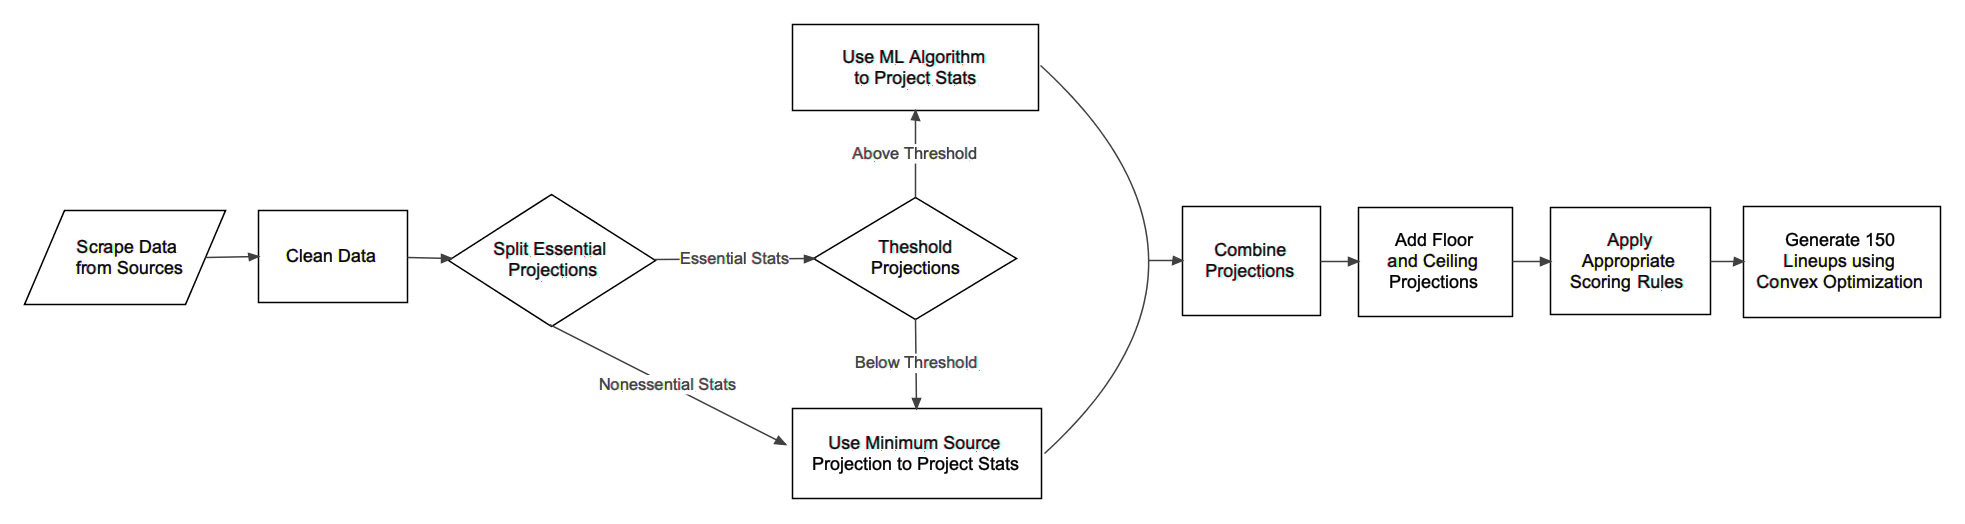
\includegraphics[width=0.95\textwidth]{../figures/pipeline}
  \caption{Full data pipeline for generating optimal lineups.}
  \label{pipeline}
\end{figure}

\pagebreak
\section{Data Summary}
TODO


\subsection{Data Collection}
\begin{table}[H]
\caption{Data collected from each source.}
\small
\label{sources}
\centering
\begin{tabular}{lcc}
	\toprule
	Source        &  Full Season              &  Weekly \\
	\midrule
	CBS           &  QB, RB, WR, TE, DST, K   &   QB, RB, WR, TE, DST, K \\
	ESPN          &  QB, RB, WR, TE, DST, K   &   QB, RB, WR, TE, DST, K \\
	FantasyPros   &  QB, RB, WR, TE, DST, K   &   QB, RB, WR, TE, DST, K \\
	FFToday       &  QB, RB, WR, TE, DST, K   &   QB, RB, WR, TE, K \\
	NFL.com       &  QB, RB, WR, TE, DST, K   &   QB, RB, WR, TE, DST, K \\
	RTSports      &  QB, RB, WR, TE, DST, K   &    {} \\
	Yahoo         &  {}                       &   QB, RB, WR, TE, DST, K \\
	\midrule
	DraftKings    &  {}                       &   QB, RB, WR, TE, DST \\
 	FanDuel       &  {}                       &   QB, RB, WR, TE, DST \\
	\bottomrule
\end{tabular}
\end{table}

For the scope of this report, full season analysis will be neglected. However, the data has been collected, allowing for potential future work on full season projections which may prove useful for season long fantasy leagues. As daily fantasy websites such as DraftKings and FanDuel do not include kickers in possible lineups, kickers will also be neglected for the remainder of this report.\bigskip

For each position, a variety of stats are projected from the various sources. Due to lack of consistency between which stats are projected and which are not among the sources, stats were broken down into two categories. The first category we denote \textit{essential stats}, stats which are projected by most of the sources and are generally non-zero in value. The second category we denote \textit{nonessential stats}, stats which may not be projected by more than a couple sources and are generally 0 or near 0 in value. Table \ref{stats table} lists the essential and nonessential stats for each position.

\begin{table}[H]
\caption{Essential and nonessential stats for each position.}
\small
\label{stats table}
\centering
\begin{adjustbox}{width =\textwidth}
\begin{tabular}{lcc}
	\toprule
	Position        &  Essential Stats            &  Nonessential Stats \\
	\midrule
	QB   &  Pass Yds, Pass TD, Pass Int, Rush Yds, Rush TD,   &   Receptions, Rec Yds, Rec TD, 2PT\\
	RB   &  Rush Yds, Rush TD, Receptions, Rec Yds, Rec TD   &   Pass Yds, Pass TD, Pass Int, 2PT \\
	WR   &  Rush Yds, Rush TD, Receptions, Rec Yds, Rec TD   &   Pass Yds, Pass TD, Pass Int, 2PT \\
	TE   &  Receptions, Rec Yds, Rec TD    &   Pass Yds, Pass TD, Pass Int, Rush Yds, Rush TD, 2PT\\
	DST  &  PA, YdA, TD, Sack, Int, Fum Rec & Saf, Blk \\
	\bottomrule
\end{tabular}
\end{adjustbox}
\end{table}


\subsection{Missing Data}

Among data collection sources, the number of players with projections was not consistent, and in many cases projections are only provided from 4 or 5 out of 6 sources for a particular player. The number of sources which provided projections for each essential stat, and the percentage of missing data are provided in Figure \ref{missing data}. Nonessential statistics are provided in the appendix. These instances were manually observed and found to not be restricted to backups, but often occur in prominent starting players (e.g., Drew Brees, Cam Newton). Since prominent players were affected, the players with missing projections could not be dropped, necessitating imputing of missing values.\bigskip


\begin{figure}[H]
  \centering
  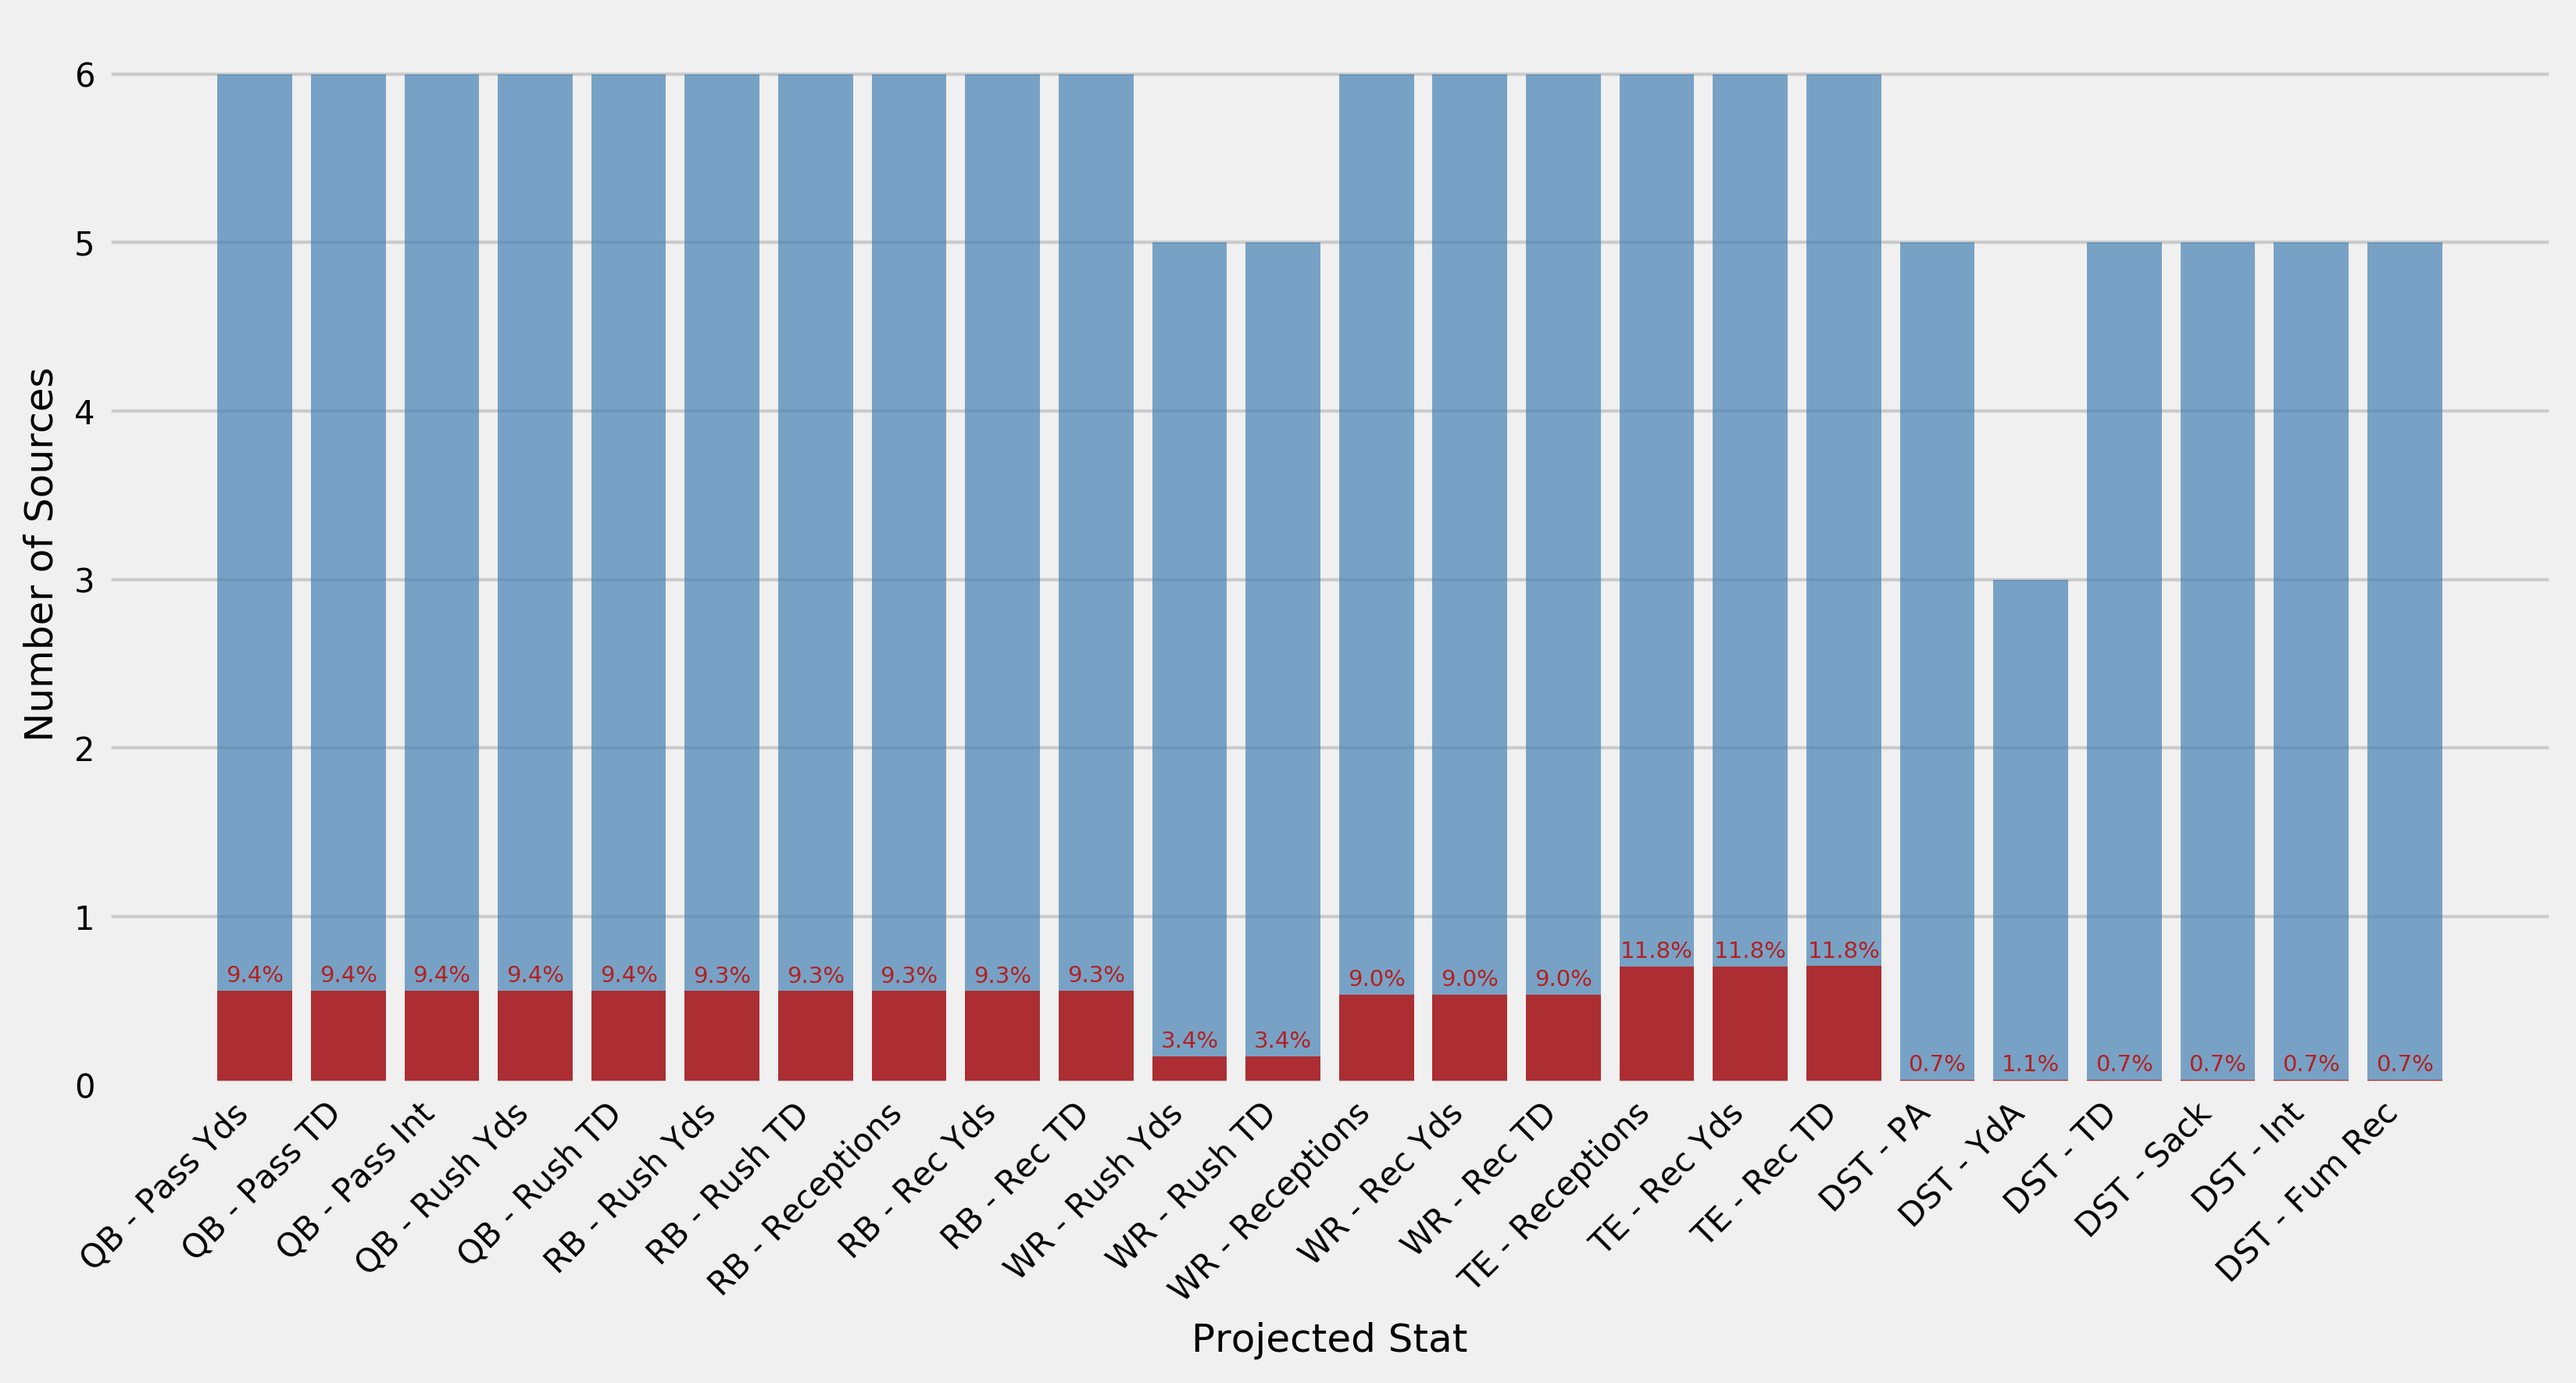
\includegraphics[width=0.95\textwidth]{../figures/missing_data}
  \caption{Number of sources collected for each essential stat (blue). Red indicates percentage of missing data for each respective stat.}
  \label{missing data}
\end{figure}

Several imputing methods were tested to find the optimal method for imputing missing projections. Imputing algorithms from the \texttt{fancyimpute} Python package were utilized to perform the imputing\cite{fancyimpute}. The simplest of these techniques as simply filling the projections from missing sources with the mean or median of the collected projections. Several more advanced methods were also studied. First, an iterative imputing method was used, where each source with missing values was first modeled as a function of all other sources using rows with full data, and these respective models were subsequently used to impute missing values for each source. Second, a K-nearest neighbors (KNN) approach was used, where each source is given a weight based on rows with all data observed. A matrix factorization approach was also studied which uses gradient descent to directly solve a factorization of the incomplete matrix into low-rank $U$ and $V$ matrices with L1 and L2 regularization respectively. Finally a soft impute method was studied which completes the matrix via soft thresholding singular value decompositions (SVD). Strictly using SVD was not possible due to the low number of sources (6) compared to the number of players which ranged from 32 for DST to upwards of 200 for WR. More information regarding each method and literature is available at \cite{fancyimpute}.\bigskip

In order to test which imputing method was best suited for the stat projection dataset, a raw matrix of all projected players for every week of the season was compiled for each stat. Players with 50\% or more sources missing were dropped, as these players were always either backups or players not expected to start, resulting in an incomplete matrix. Next, the percentage of missing data in the incomplete matrix for each respective stat was recorded, shown in Figure \ref{missing data}. All rows (players) with any missing values were subsequently removed, leaving a fully completed matrix for each stat. Elements in this completed matrix were then removed at random until the matrix had an equivalent missing data percentage as incomplete matrix. Each imputation method described above was then used to impute these missing values, with the mean average error (MAE) and root mean squared error (RMSE) recorded for the difference between the imputed matrix of each method and the complete matrix of true projection values. This process was repeated for 50 simulations in order to reduce potential variation from the random selection of missing elements. The resulting MAE and RMSE values for each imputing method of the essential stats is provided below. 


\begin{figure}[H]
  \centering
  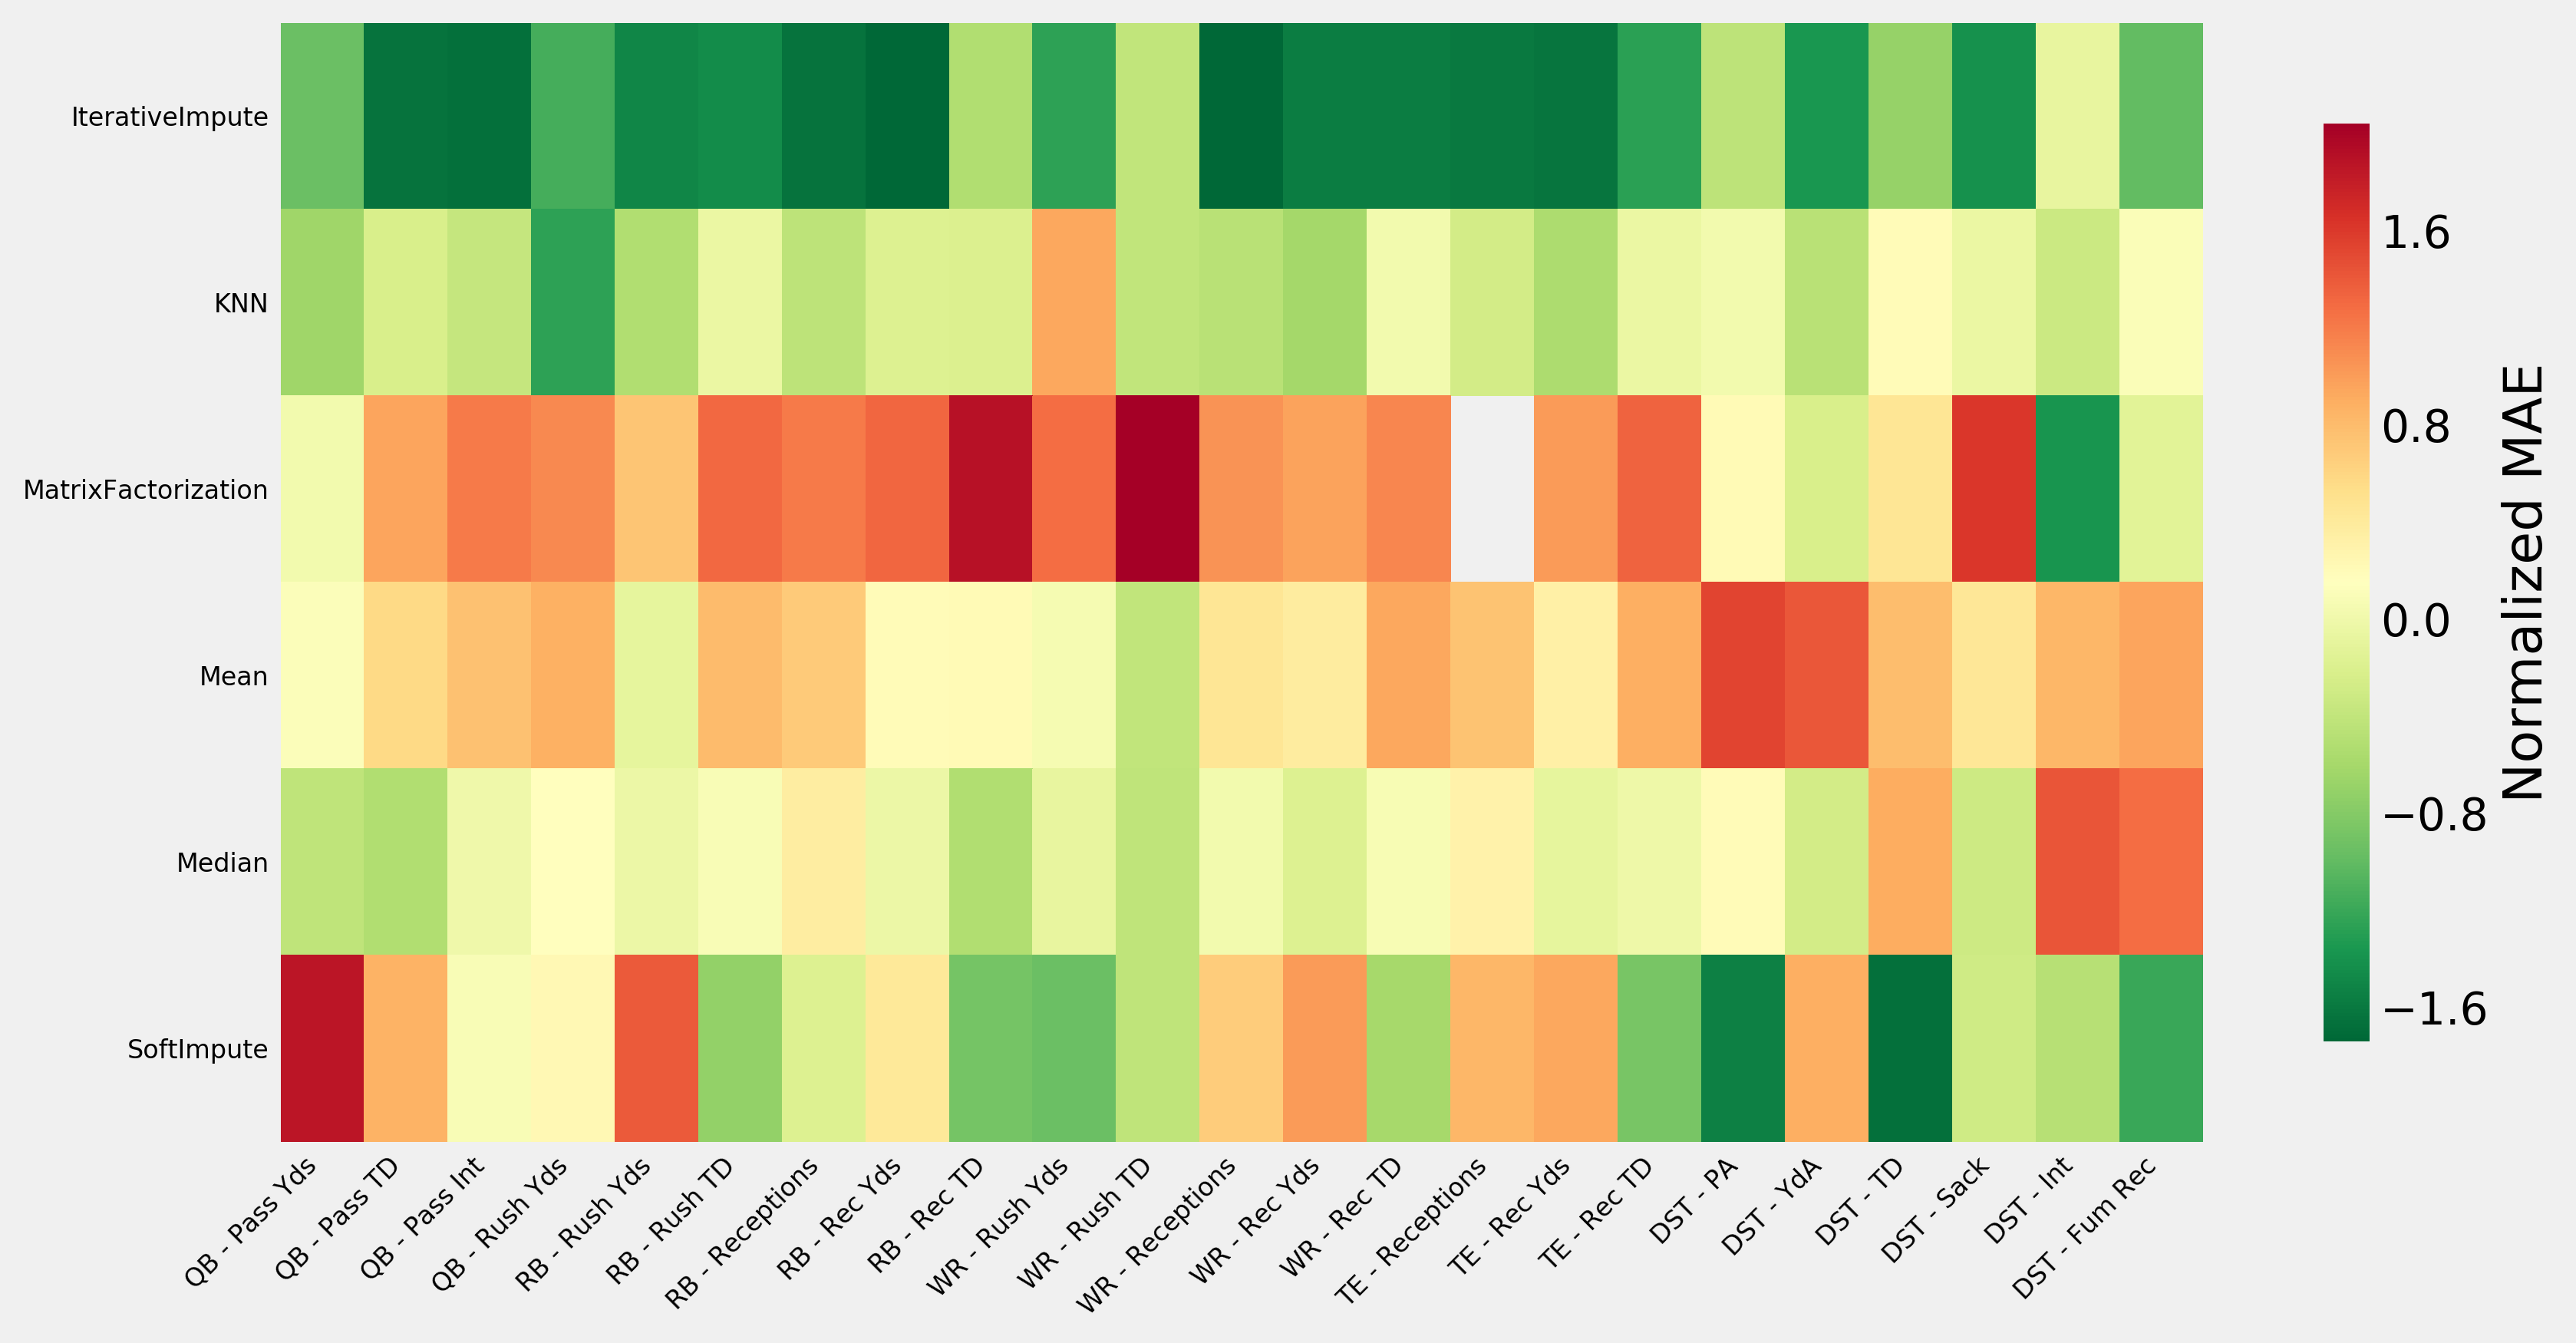
\includegraphics[width=0.95\textwidth]{../figures/impute_MAE}
  \caption{Normalized MAE of imputing methods for each essential stat.}
  \label{impute MAE}
\end{figure}

\begin{figure}[H]
  \centering
  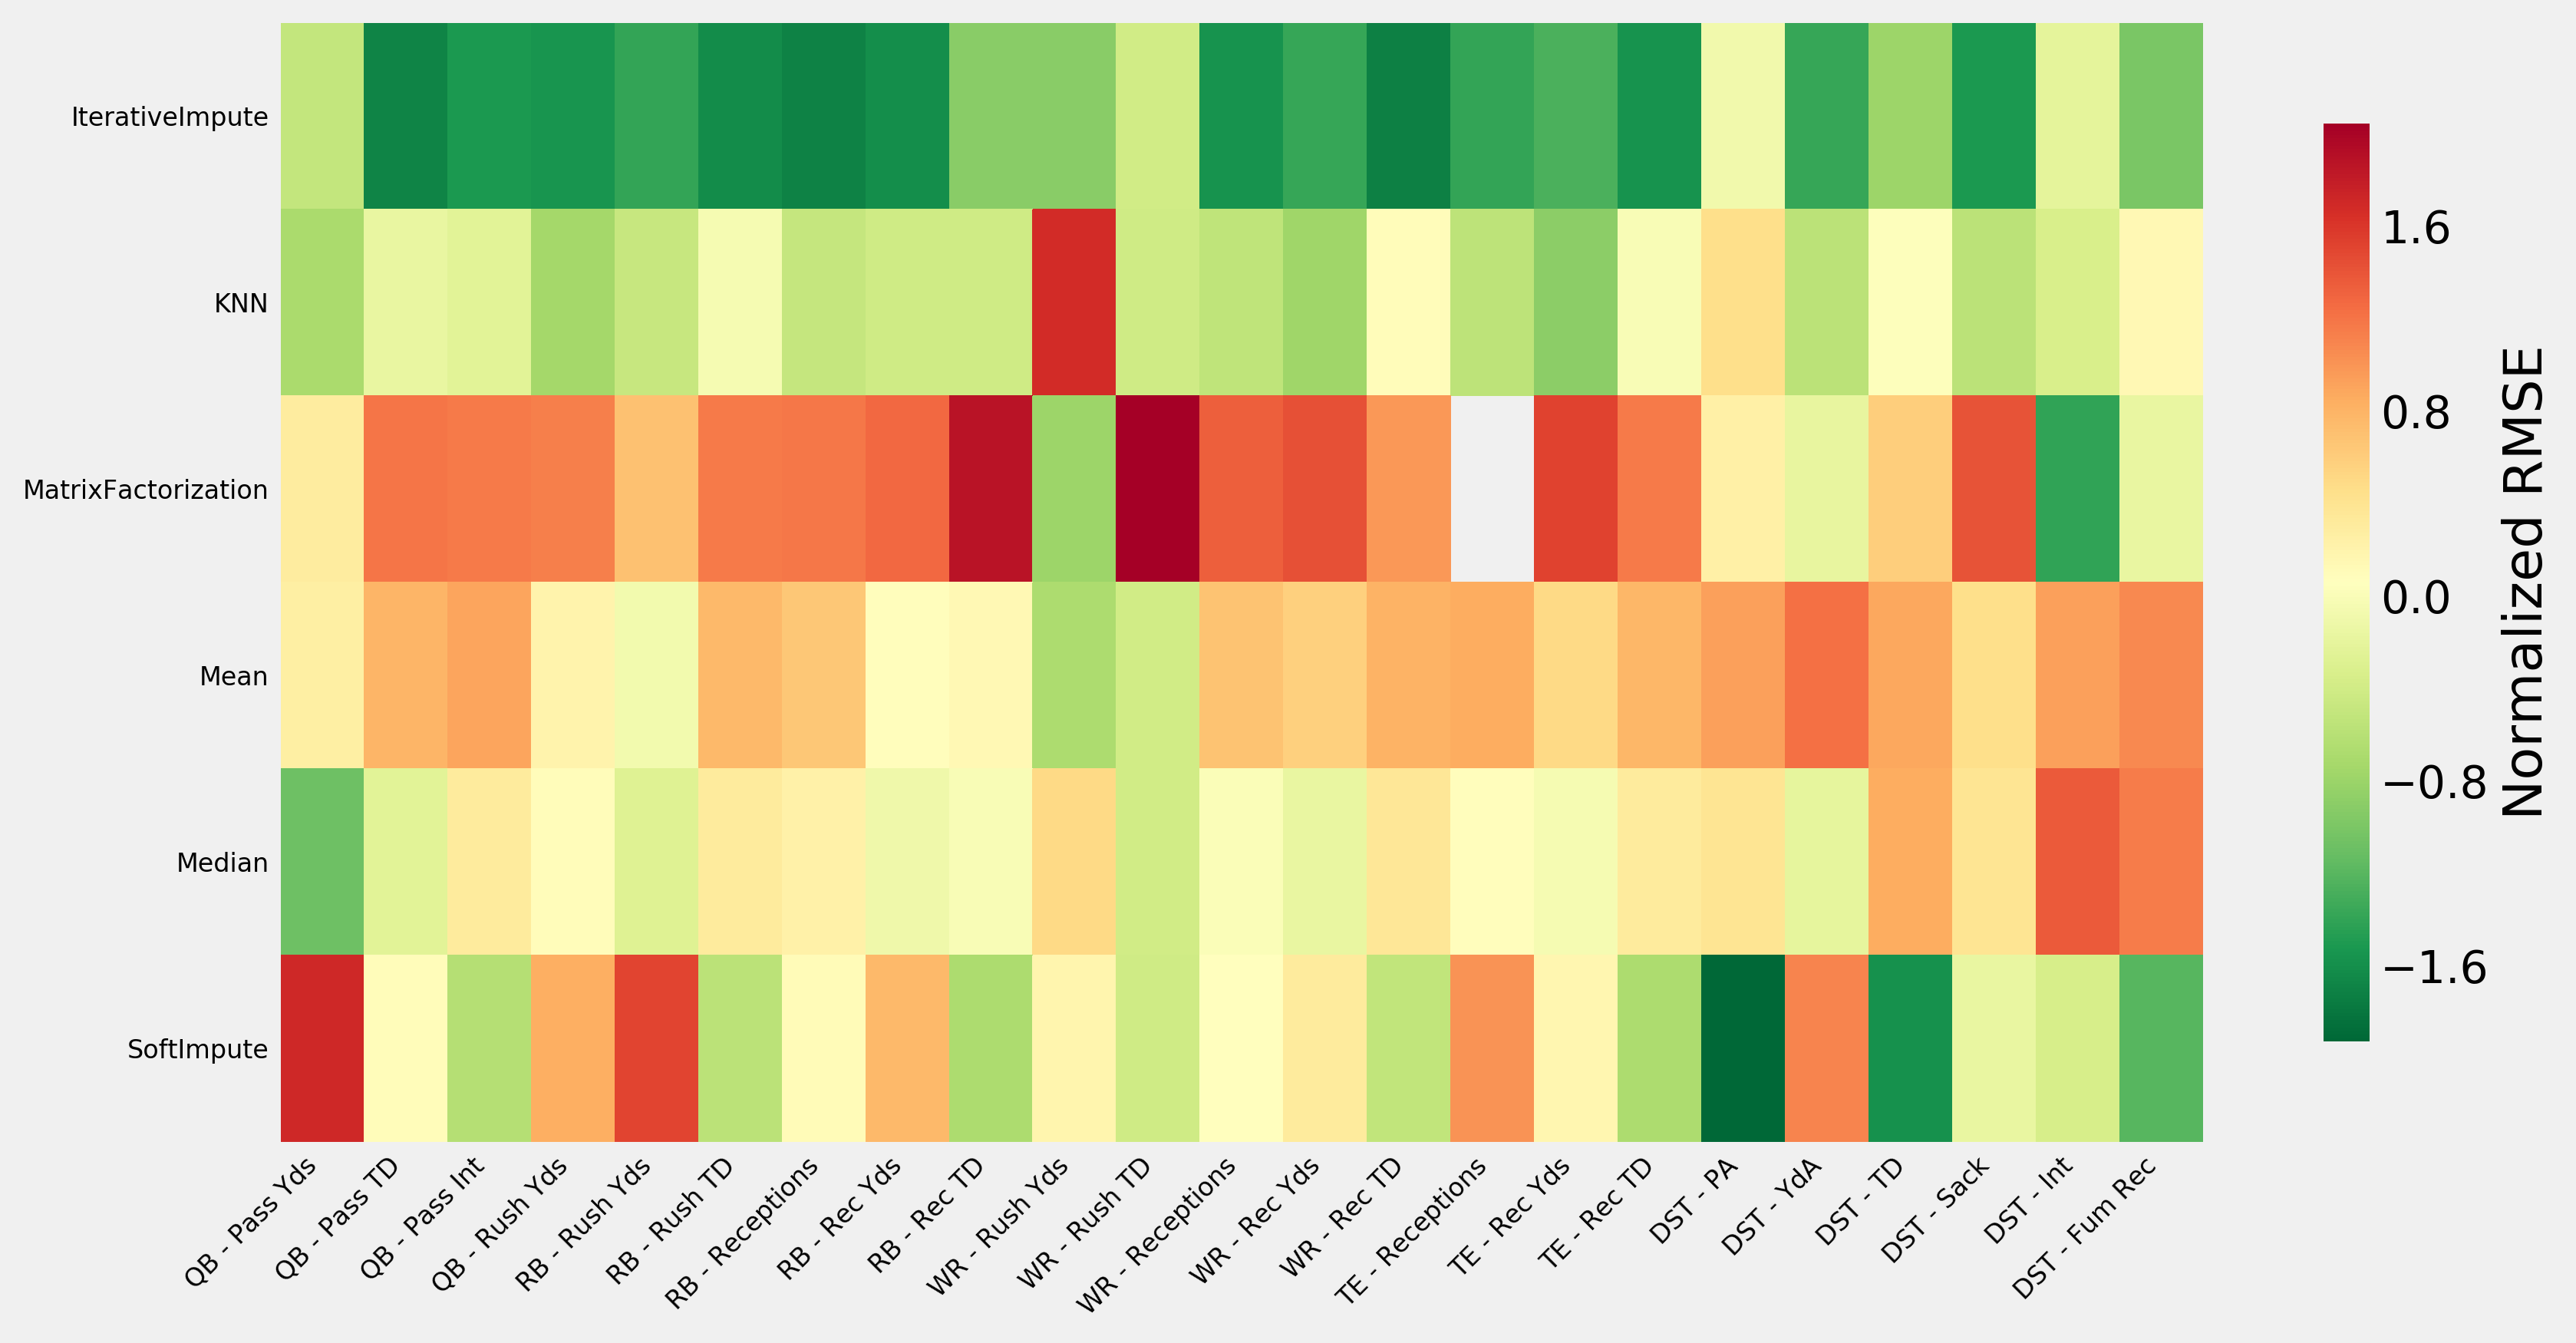
\includegraphics[width=0.95\textwidth]{../figures/impute_RMSE}
  \caption{Normalized RMSE of imputing methods for each essential stat.}
  \label{impute RMSE}
\end{figure}

Figures \ref{impute MAE} and \ref{impute RMSE} clearly indicate that the iterative imputing method provides the best estimates for missing values.  A comparison of imputing techniques for nonessential stats is provided in the appendix, where iterative imputing was again found to be optimal. Therefore iterative imputing was used to impute missing values for both essential and nonessential stats for the remainder of this study.

\subsection{Data Exploration}

The raw values for realized stats were investigated prior to building predictive models. For each stat, two nearly independent distributions were observed, one near zero and the other significantly different than zero. These two distributions were identified as \textit{starters} and \textit{backups} (i.e., players who were expected to play the entire game and players who come of the bench and play a minimal role respectively). Due to the difficulties that would arise from machine learning models attempting to predict multiple distributions, a threshold was set for each stat to separate values from starters and backups. Separate models were used to predict stats above and below these thresholds, both of which will be discussed further in the methodology section. Thresholds were selected manually through observation of histograms of each stat. Figure \ref{example hist pass yds} displays an example threshold for an easily separable stat, Pass Yds, where the two distributions are clearly distinguishable. Figure \ref{example hist rush yds} displays an example threshold for a more difficult stat to separate, Rush Yds, which appears to have three distributions, one near zero, one linear decreasing, and a third bell shape distribution. For stats such as Rush Yds, the separation boundary was chosen to separate near-zero and non-zero distributions to avoid having numerous categorical distributions within each stat. The selected thresholds and resulting histograms after thresholding for all essential stats are provided in the appendix.


\begin{figure}[H]
  \centering
  \begin{subfigure}[b]{0.450\textwidth}
    \centering
    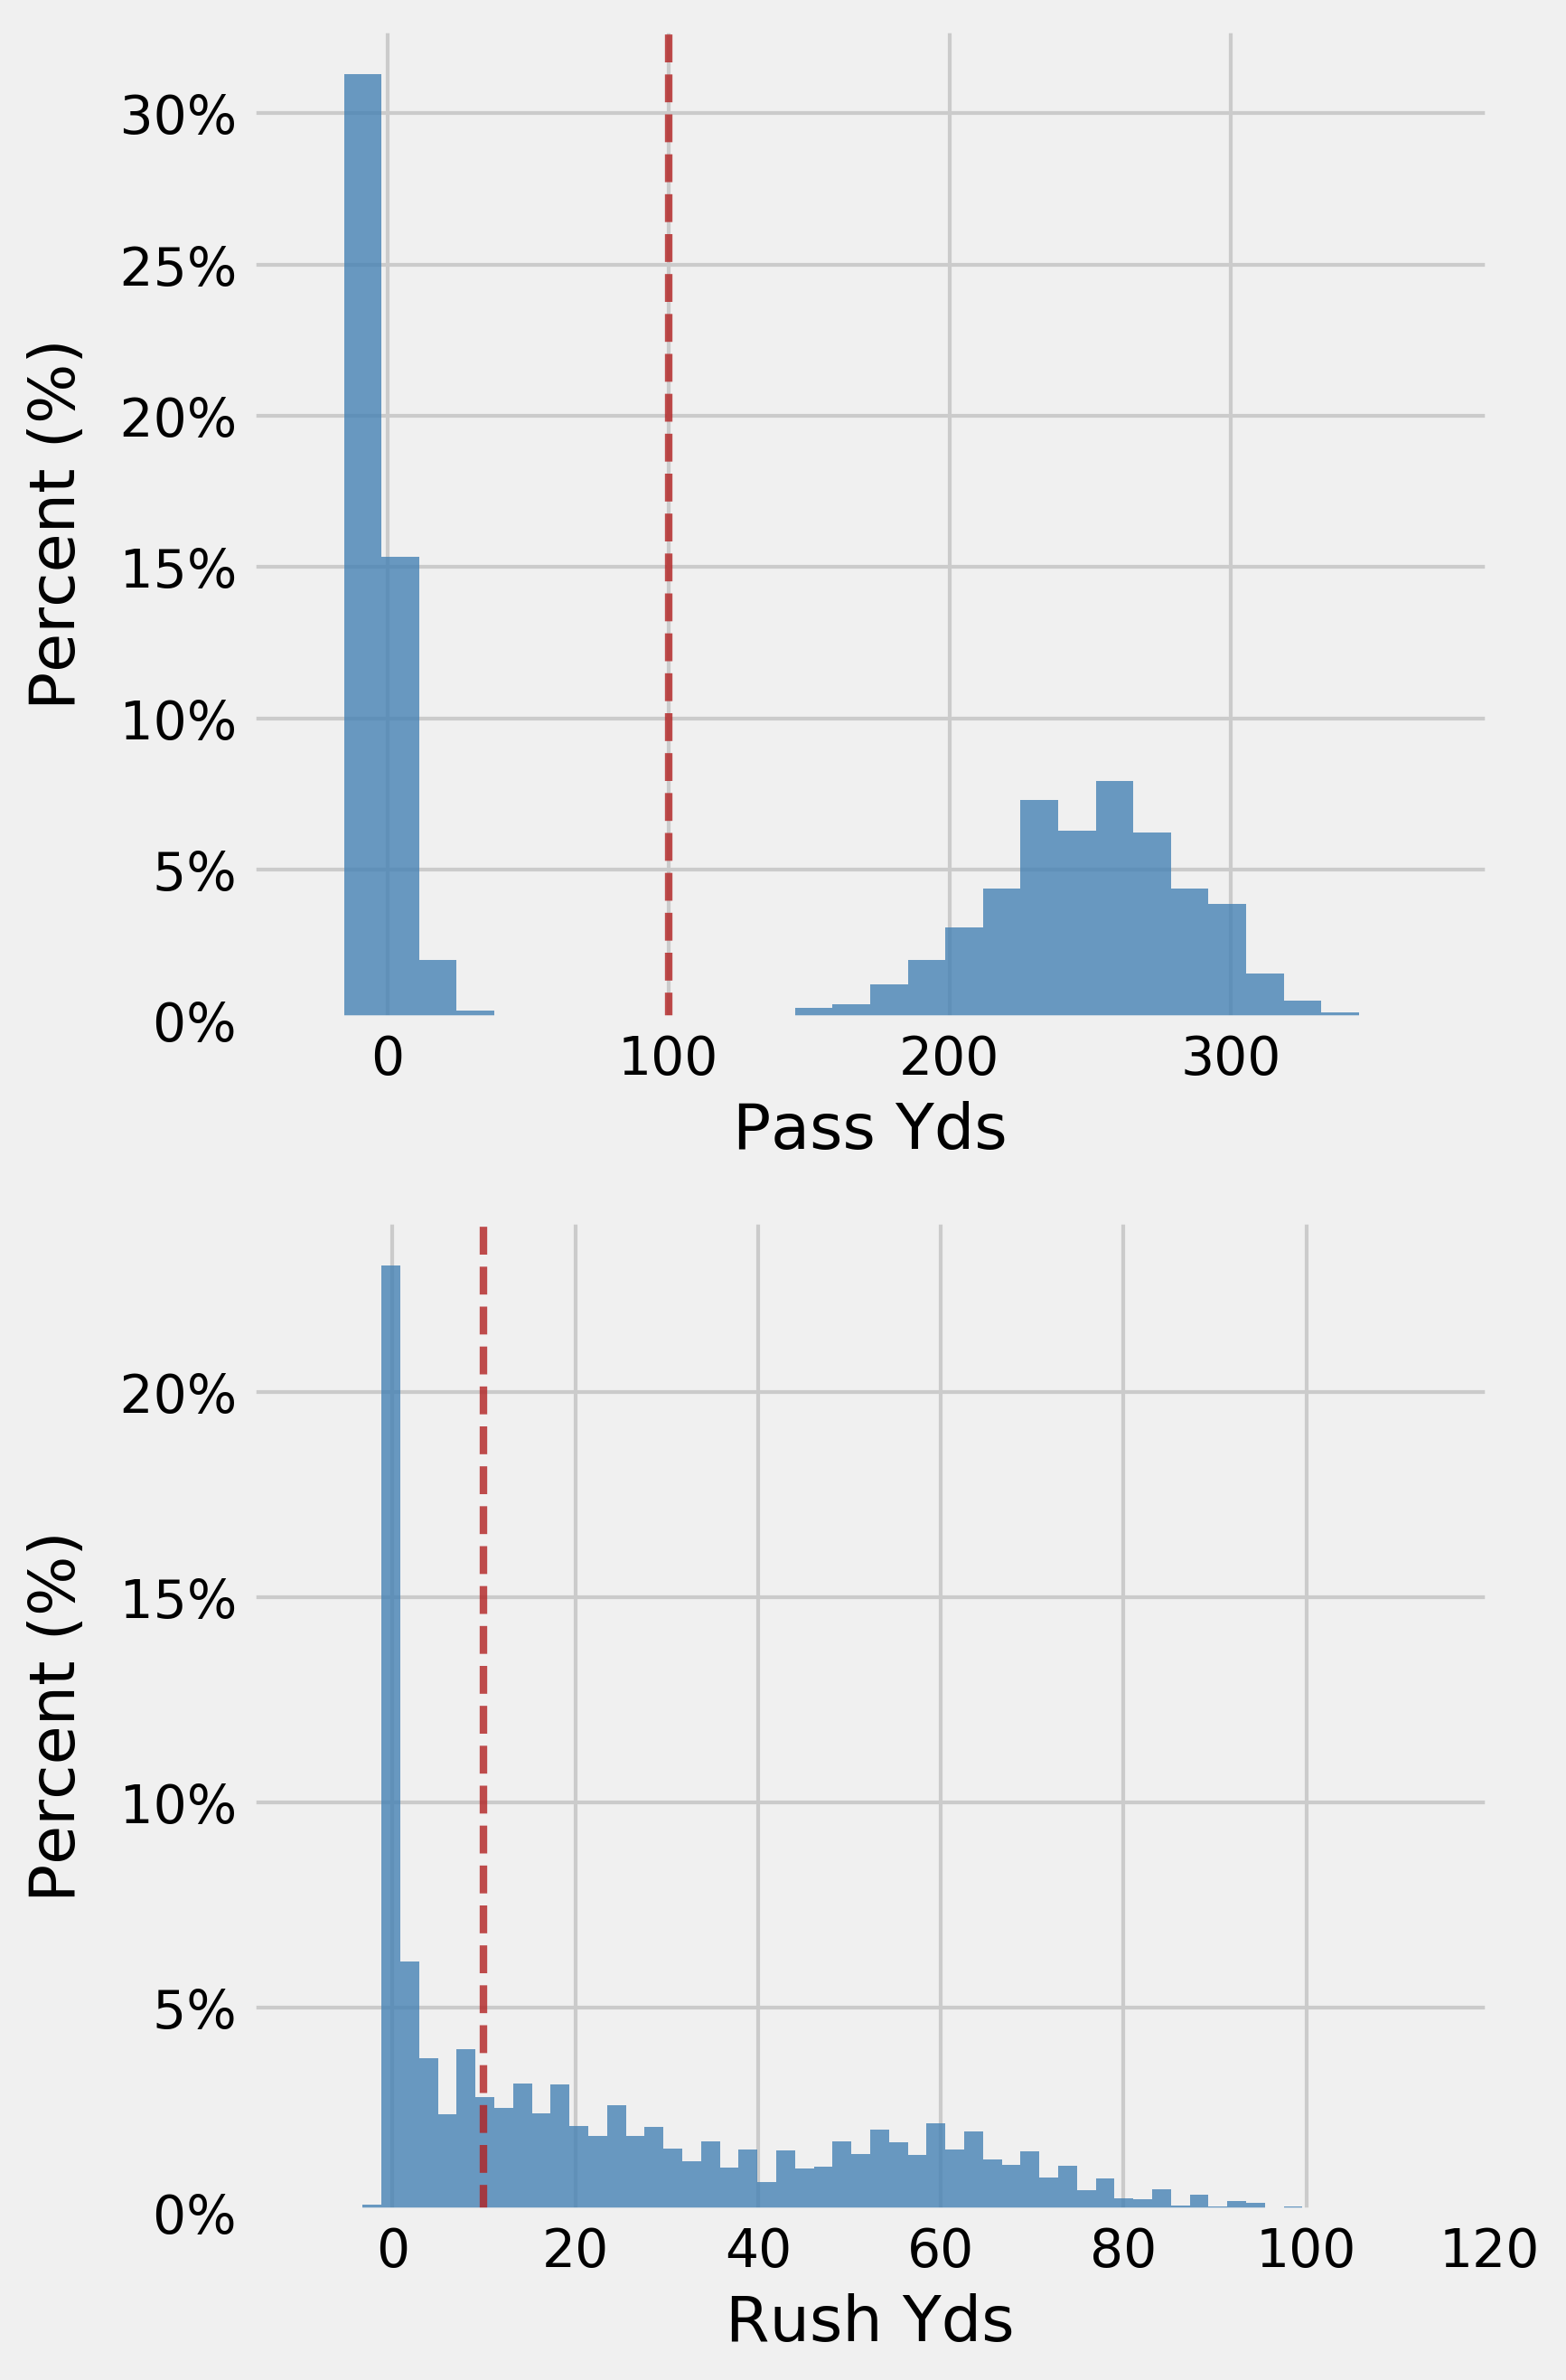
\includegraphics[width=1\textwidth]{../figures/no_theshold_example_hists}
    \caption{Raw histogram with threshold (red).}
    \label{example hist pass yds}
  \end{subfigure}
  \hfill
  \begin{subfigure}[b]{0.450\textwidth}
    \centering
    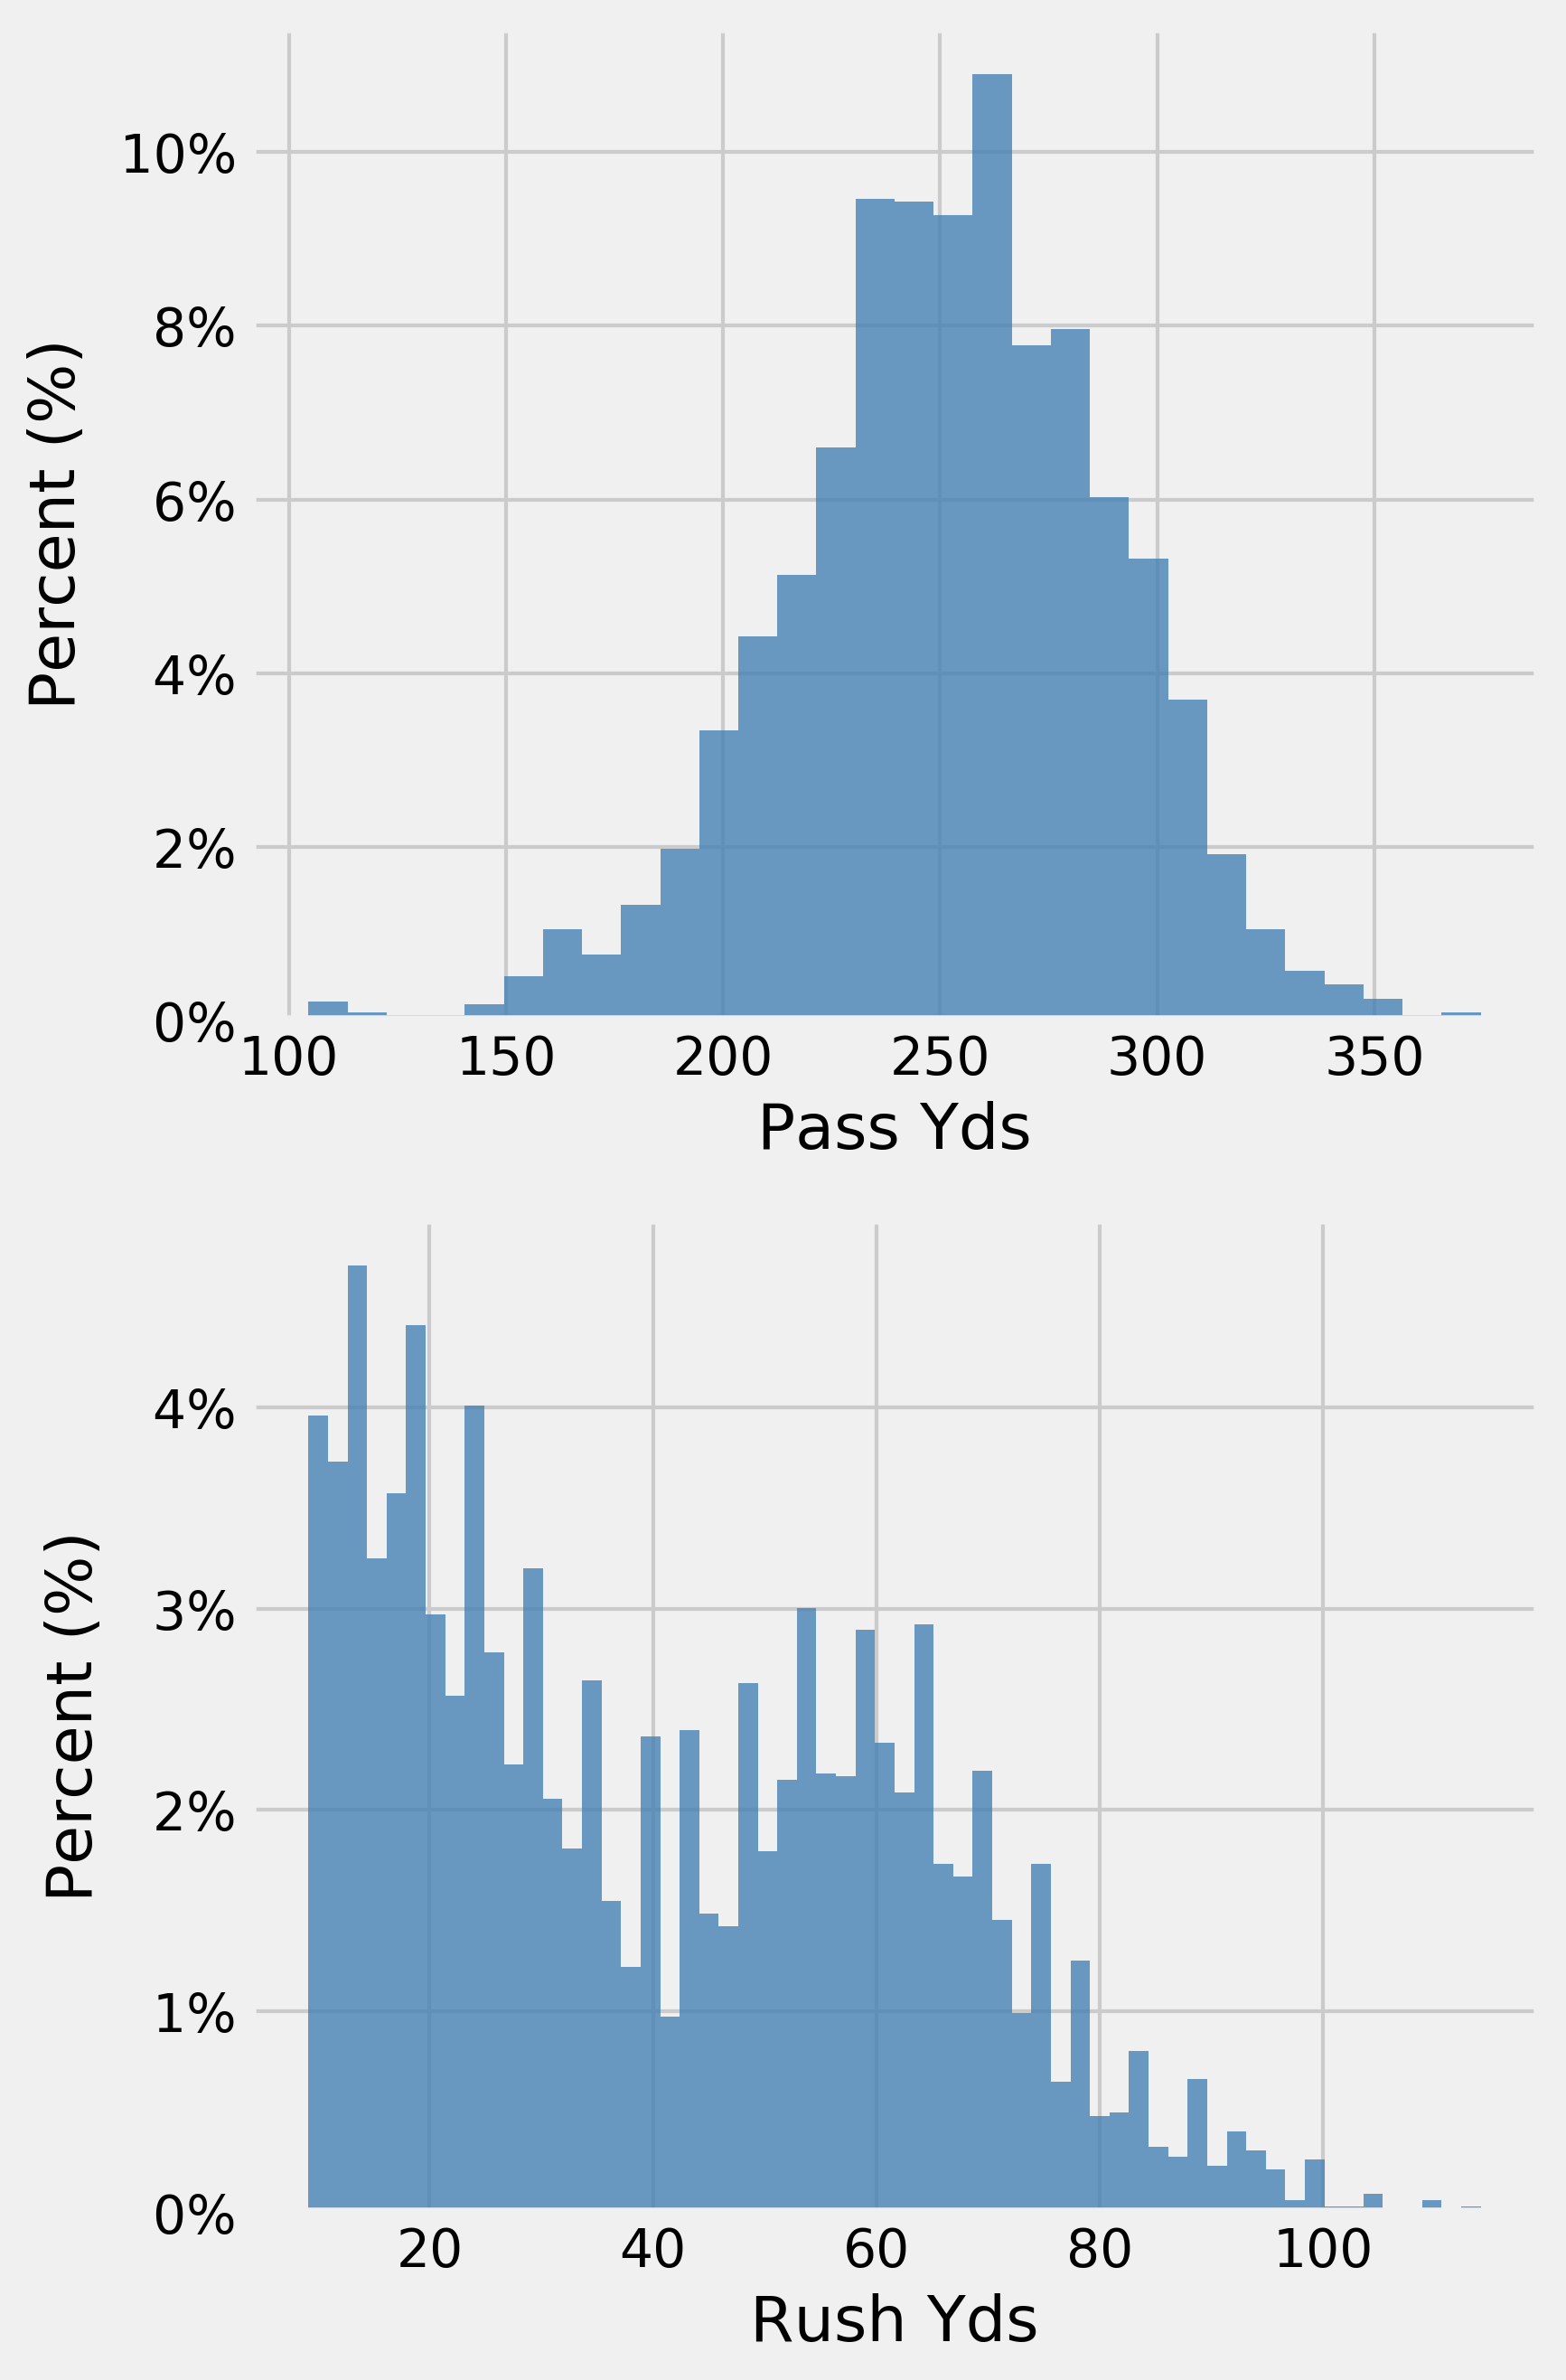
\includegraphics[width=1\textwidth]{../figures/no_theshold_example_hists_RB}
    \caption{Histogram above threshold.}
     \label{example hist rush yds}
  \end{subfigure}
  \caption{Example raw and thresholded histograms for QB passing yards and RB rushing yards.}
  
\end{figure}


\pagebreak
\section{Methodology}


\subsection{Projections}
In order to project scores for each player, the individual stats of that player were projected, and subsequently combined with scoring rules for either FanDuel or DraftKings to generate a final scoring projection for each week. Models used for individual stat projections were trained on a \textit{training} period (Weeks 1-11), validated on a \textit{cross-validation} period (Weeks 12-14), and finally tested on an unseen \textit{testing} period (Weeks 15-17). This train/cross-validation/test procedure is the standard in machine learning literature as it ensures models are not overfit to the training data, establishes a unseen period to identify the best model in the cross-validation period, and can be tested on completely unseen data in the test period, providing a fair estimate for how well the model will do given future data.\bigskip

For all stats, the projections from individual sources were used as feature variables for the final projection. More concretely, for a given stat such as Pass Yds, the feature variable vector $X = [\text{CBS},\ \text{ESPN},\ \text{FantasyPros},\ \text{FFToday},\ \text{NFL},\ \text{RTSports},\ \text{Yahoo}]$ where each source name represents the Pass Yds projection from that respective source. Given the feature variable vector, the projection $y$ can be found:
\begin{equation}
y = f(X)
\end{equation}
where $f(\cdot)$ can be any function. The studied functions used to form projections are given in Table \ref{ML algos}.

\begin{table}[H]
\caption{Functions and algorithms used to project stats from feature variables.}
\label{ML algos}
\centering
\begin{tabular}{llc}
	\toprule
	Abbreviation        &  Name           &  Source \\
	\midrule
	Min		& Minimum		& -\\
	Max		& Maximum		& -\\
	Mean		& Mean		& -\\
	Median		& Median		& -\\
	LR  & Linear Regression (Elastic Net)  & \cite{LR paper, LR algo}\\
	XGB & eXtreme Gradient Boosted Trees  & \cite{XGB paper, XGB algo}\\
	OLS & Ordinary Least Squares  & \cite{OLS algo}\\
	RF & Random Forest Regressor & \cite{RF paper, RF algo}\\
	SVR & Support Vector Regressor  & \cite{SVR paper, SVR algo}\\
	\bottomrule
\end{tabular}
\end{table}

For nonessential stats, only simple methods were compared, as most stats did not have enough sources providing projections to incorporate machine learning models. The MAE results for these simple methods are provided below. As the minimum projection provided the lowest MAE for each stat with multiple projections, it was selected as the projection function for all nonessential stats.

\begin{figure}[H]
  \centering
  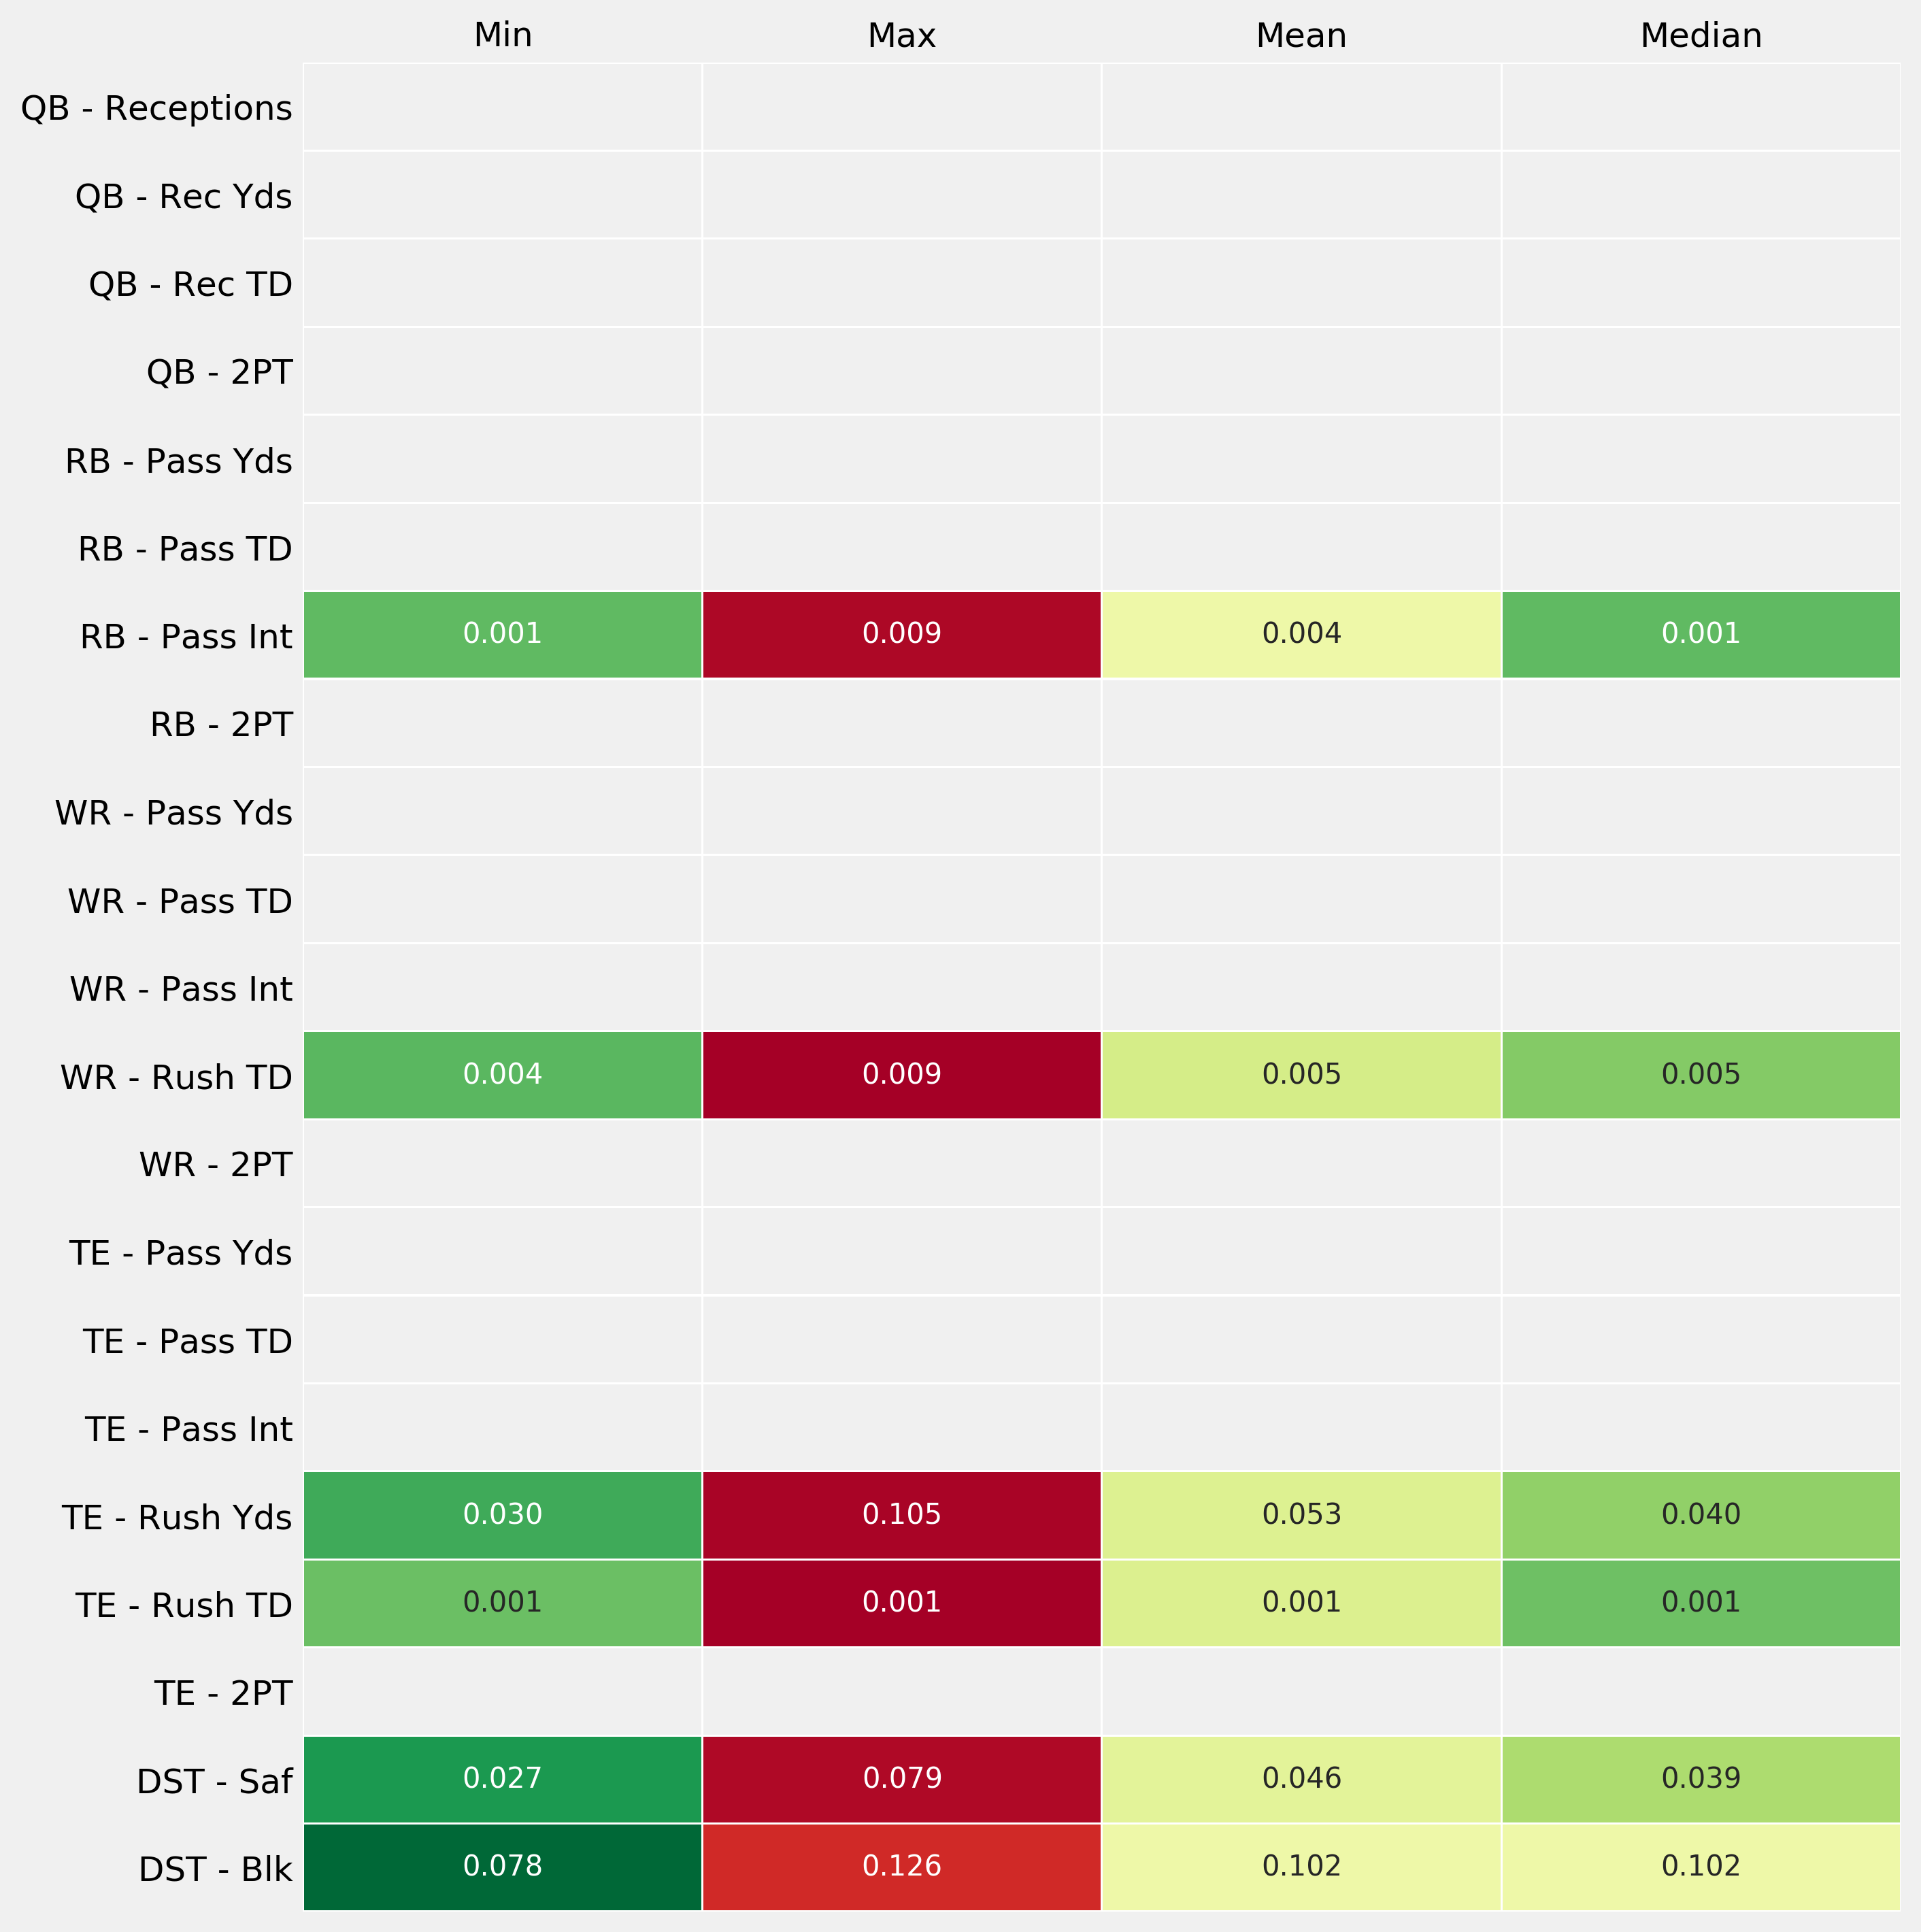
\includegraphics[width=0.8\textwidth]{../figures/nonessential_MAE_table}
  \caption{Training set MAE of simple projection methods for nonessential stats.}
\end{figure}


Similarly, essential stats below the threshold values were projected using only simple methods. Since the values were all near-zero, the added complexity of using more advanced methods would not result in much benefit to the final scoring projection for each player. As with nonessential stats, the minimum projection for stats below the specified threshold provided the lowest MAE, so minimum was the function selected for projection of stats when the mean of source projections was below the respective specified stat threshold.

\begin{figure}[H]
  \centering
  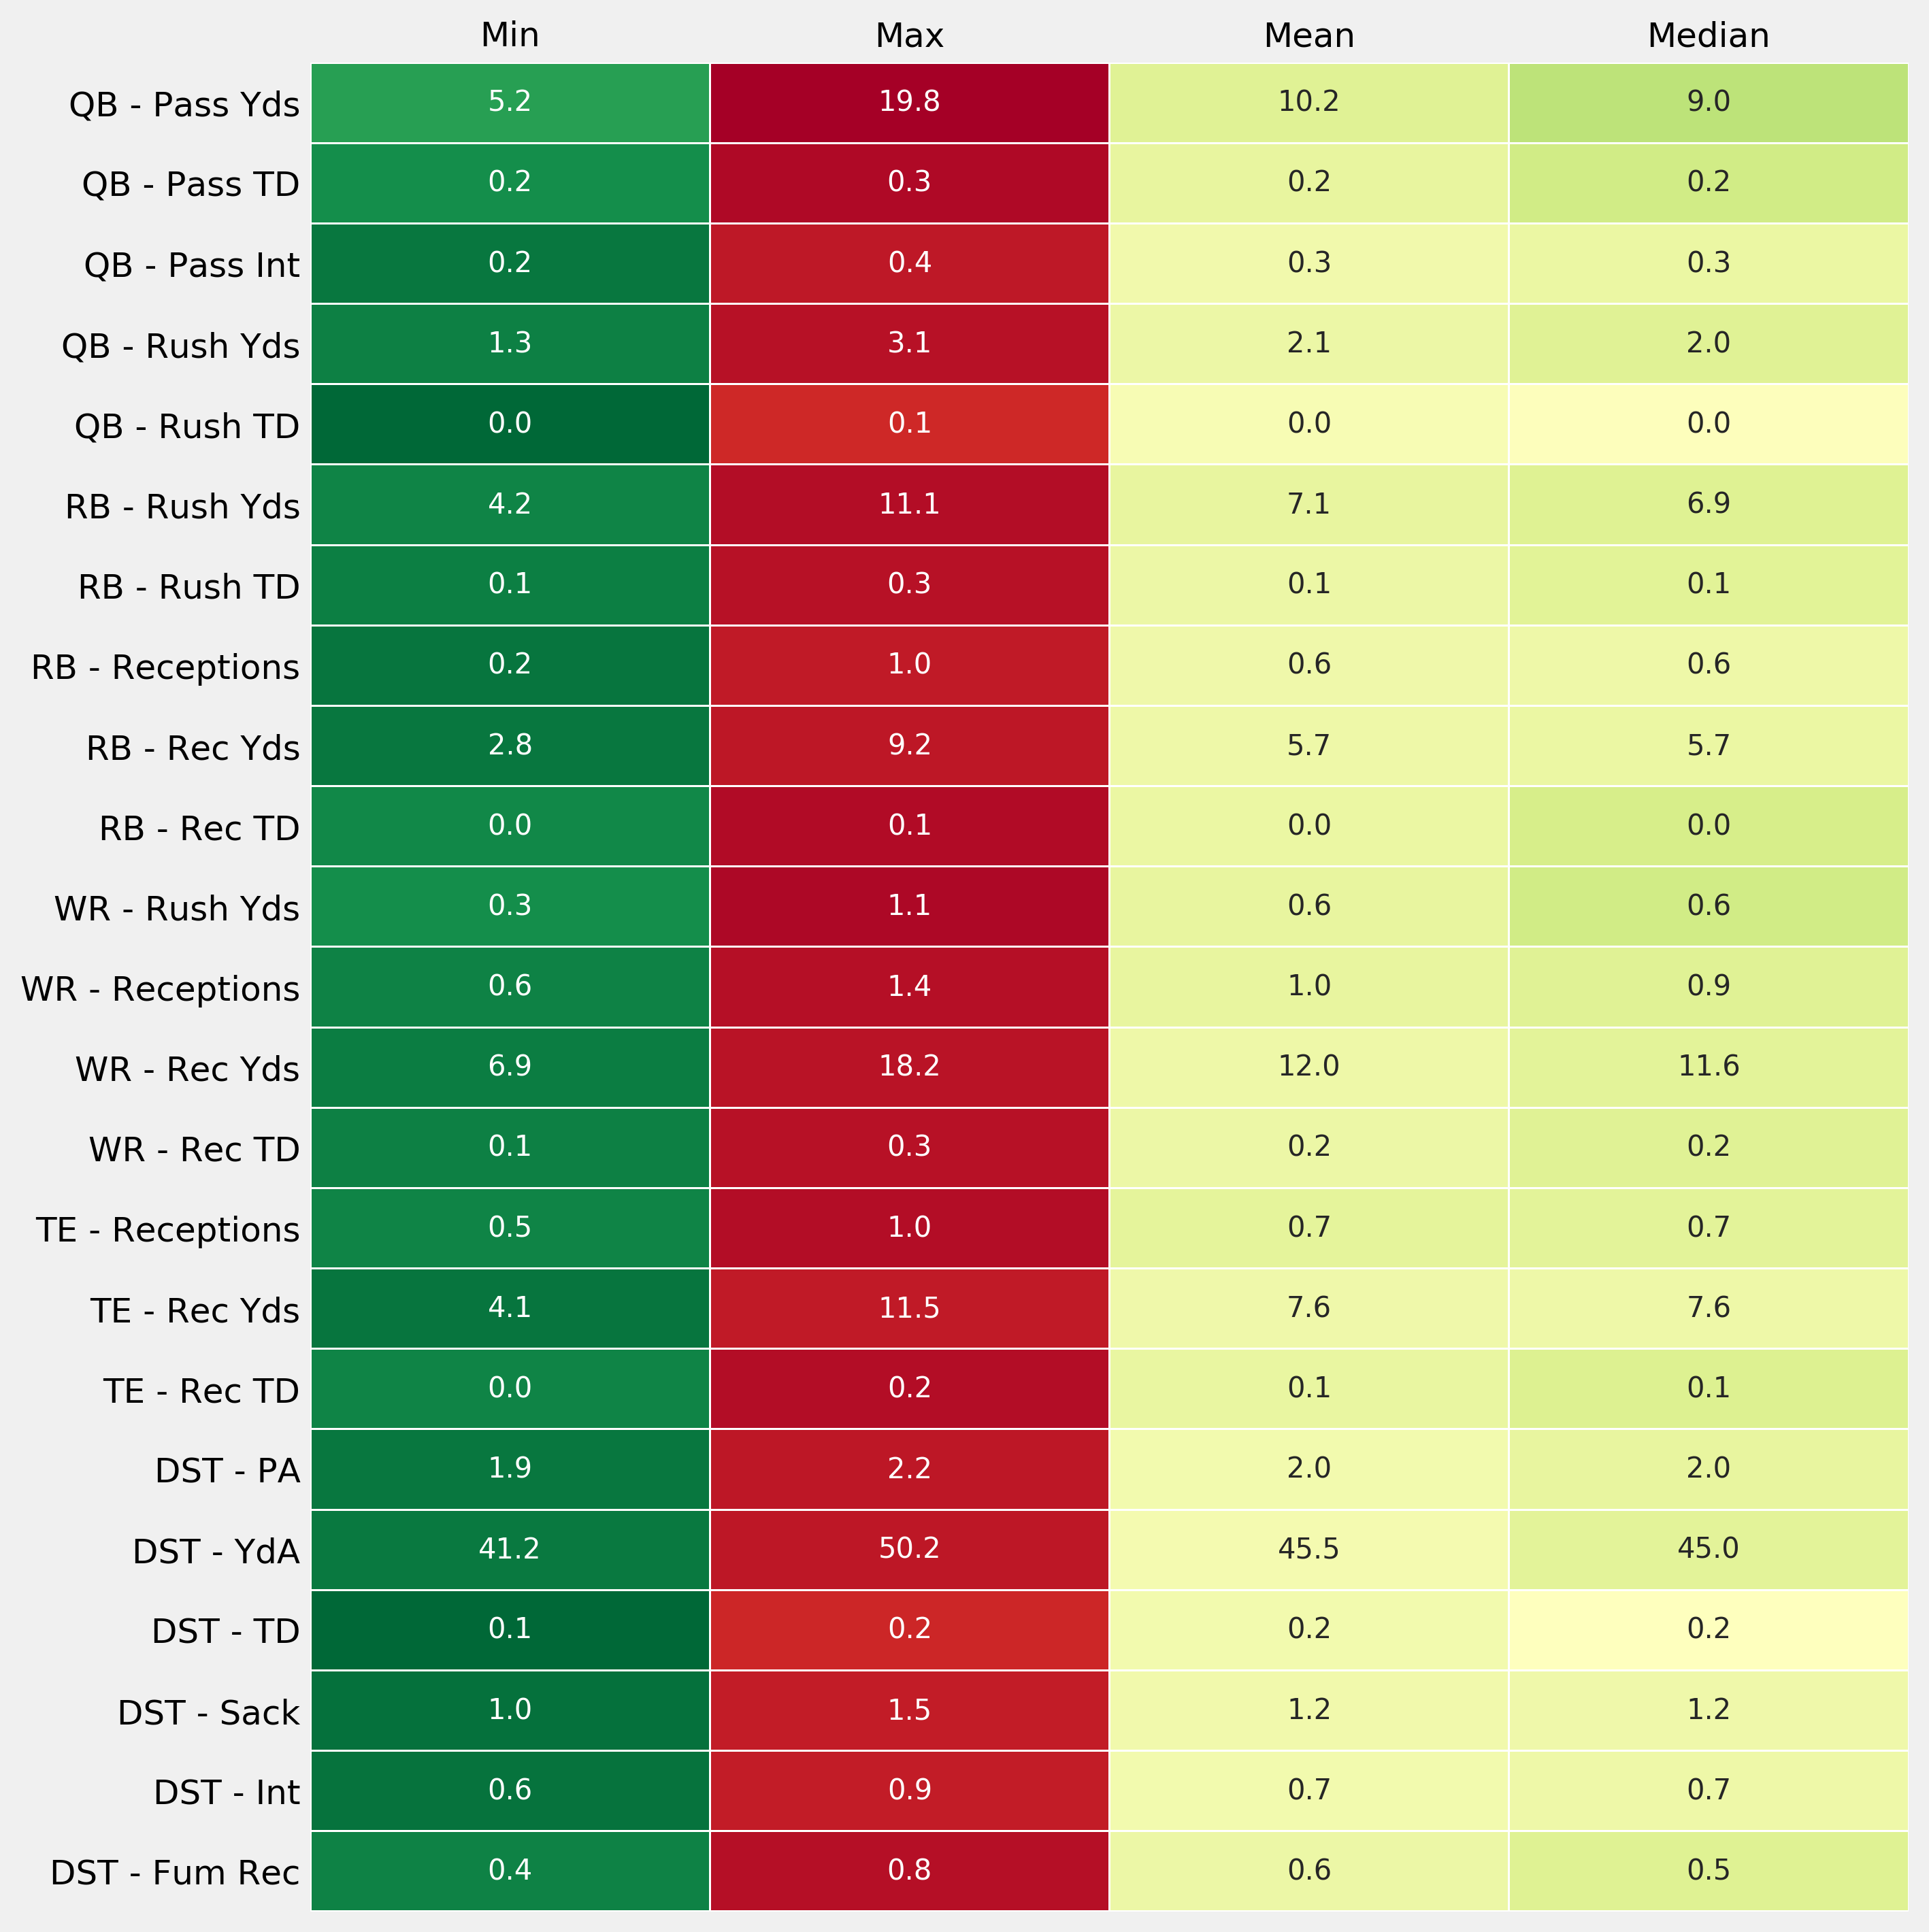
\includegraphics[width=0.8\textwidth]{../figures/essential_thresh_MAE_table}
  \caption{Training set MAE of simple projection methods for essential stats below respective stat thresholds.}
\end{figure}

Finally, essential stats above the specified thresholds were projected using the full set of studied algorithms. First, OLS was fit to the training set for each stat, which provides a simple linear approximation for the influence of each feature variable on the final projection $y$. OLS is often used as a base machine learning model since it is the simplest model with small chance of overfitting. OLS results are reported in the appendix, where the significance of each individual source for every stat is additionally provided. Note that the significance indicated is only for the \textit{linear} relation between each respective source and the true realized stat values, and sources that are deemed insignificant by OLS may still be significantly related to the true value by another degree (e.g., ESPN's projection for Pass Yds may be insignificant linearly but the square of ESPN's projection may be informative).\bigskip

In order to find these more complex relationships between source projections and realized stat values, the machine learning algorithms detailed in Table \ref{ML algos} were implemented. More information about the individual machine learning algorithms can be found in the cited references. Each stat was treated as a separate dataset, with the methodology outlined below applied to each individually as shown in Figure \ref{ML pipeline}.\bigskip

\begin{figure}[H]
  \centering
  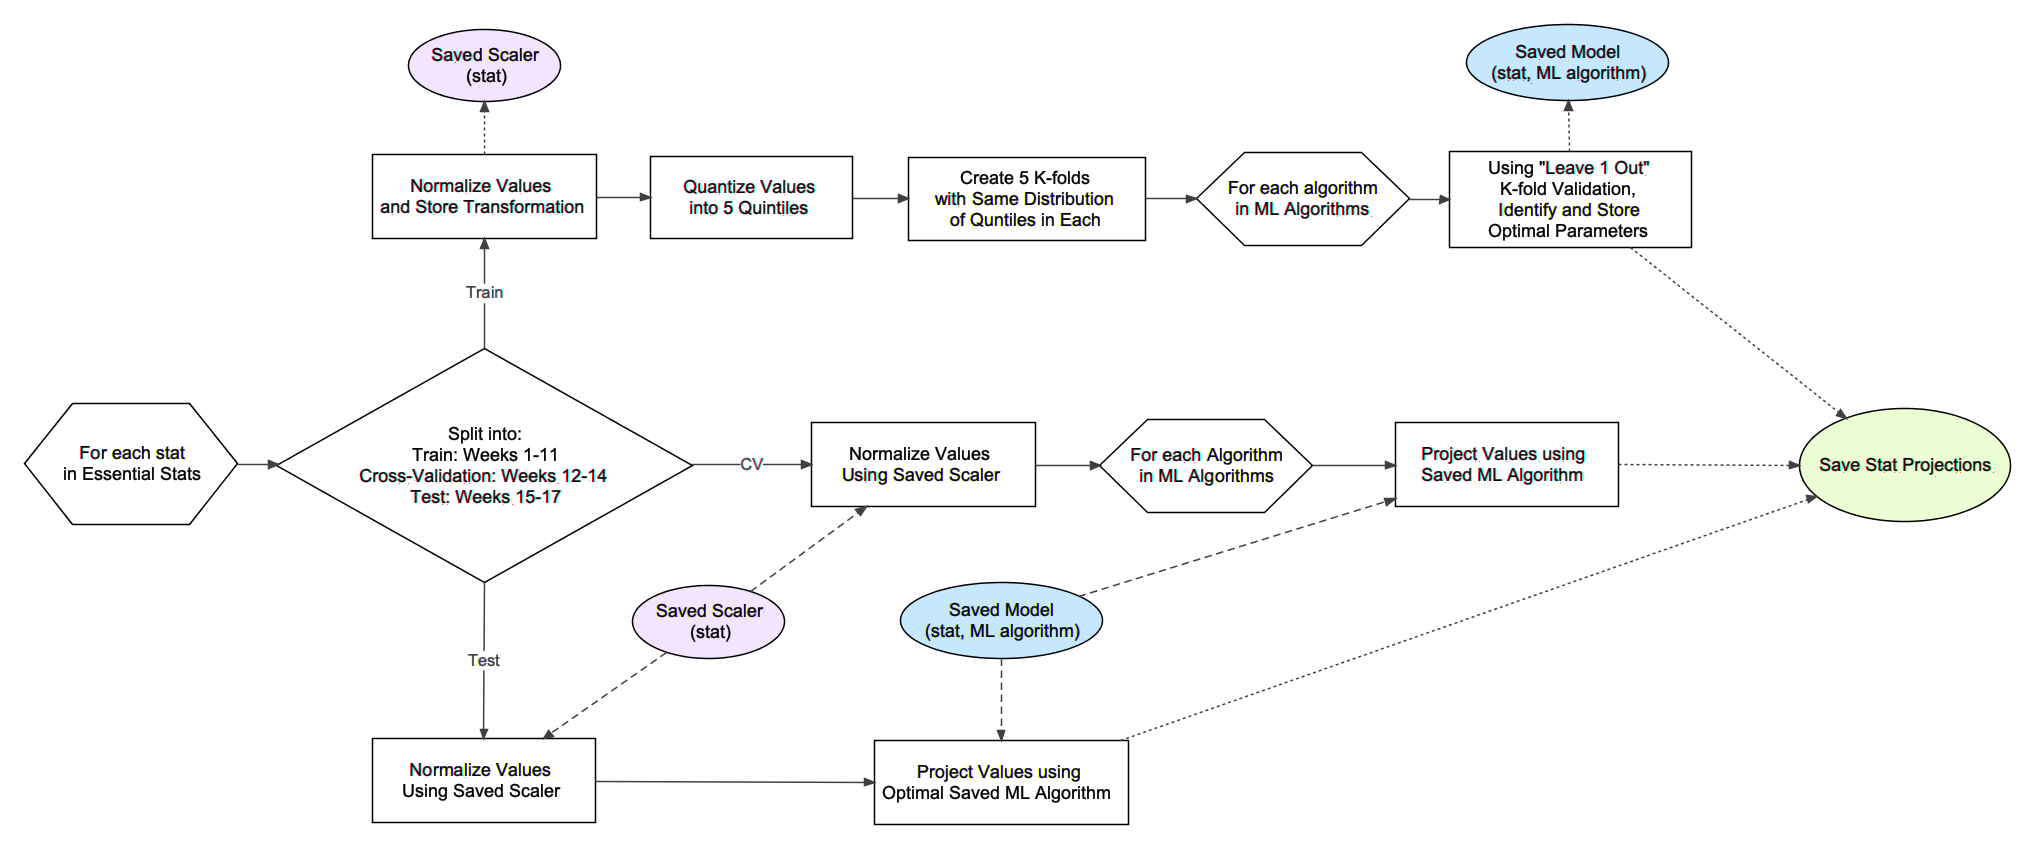
\includegraphics[width=0.95\textwidth]{../figures/ML_flowchart}
  \caption{Pipeline of machine learning generated projections. Color is used to show when models are saved and loaded.}
  \label{ML pipeline}
\end{figure}

Each machine learning model was trained using the training set of data (Weeks 1-11). Since several of the models tend to provide better estimates on similarly scaled data, the data was normalized using the training set mean and standard deviation for each stat:
\begin{equation}
X_{scaled} = \dfrac{X - \mu (X)}{\sigma (X)}
\end{equation}
where $mu$ and $\sigma$ denote the mean and standard deviation of $X$ projections for each source respectively. This scaling results in each $X_{scaled}$ having mean 0 and standard deviation of 1.\bigskip

Once the values for each stat were scaled, they were quantized into quintiles (i.e., given a categorical value 1-5 depending on if they were in the 0-20, 20-40, ..., 80-100 percentile of projections). Next, the full training data was randomly split into 5 subsets, each of which had an identical number of values from each quantile, known as a stratified shuffle split. Stratifying the split using quintiles ensures that each subset had a similar distribution of high, medium, and low values, balancing each subset. Next, a randomized cross-validation grid search was used on the first 4 subsets to find an optimal model, and tested on the fifth subset to observe the how the model performed on unseen data. This was repeated for each group of 4 subsets, known as K-fold cross-validation, to help the models generalize to unseen data. Optimal model hyperparameters from the randomized grid search were chosen from the hyperparameters which performed best on average over each of the 5 K-folds, where MAE was used as loss function. Once model hyperparameters were found for each model, they were saved to files such that they could be loaded and applied to other datasets.\bigskip

After all model hyperparameters where found for each stat, the cross-validation set (Weeks 12-14) were loaded. The saved scaling function mean and standard deviation from the training sets were then applied to scale the cross-validation data in the same manner as the training data. Following, all machine learning models were loaded and applied to the scaled data, generating projections on data previously unseen by the machine learning models which had no impact on hyperparameter selection. The resulting MAE for each stat and projection function is provided in Figure \ref{train/cv MAE}.

\begin{figure}[H]
  \centering
  \begin{subfigure}[b]{0.490\textwidth}
    \centering
    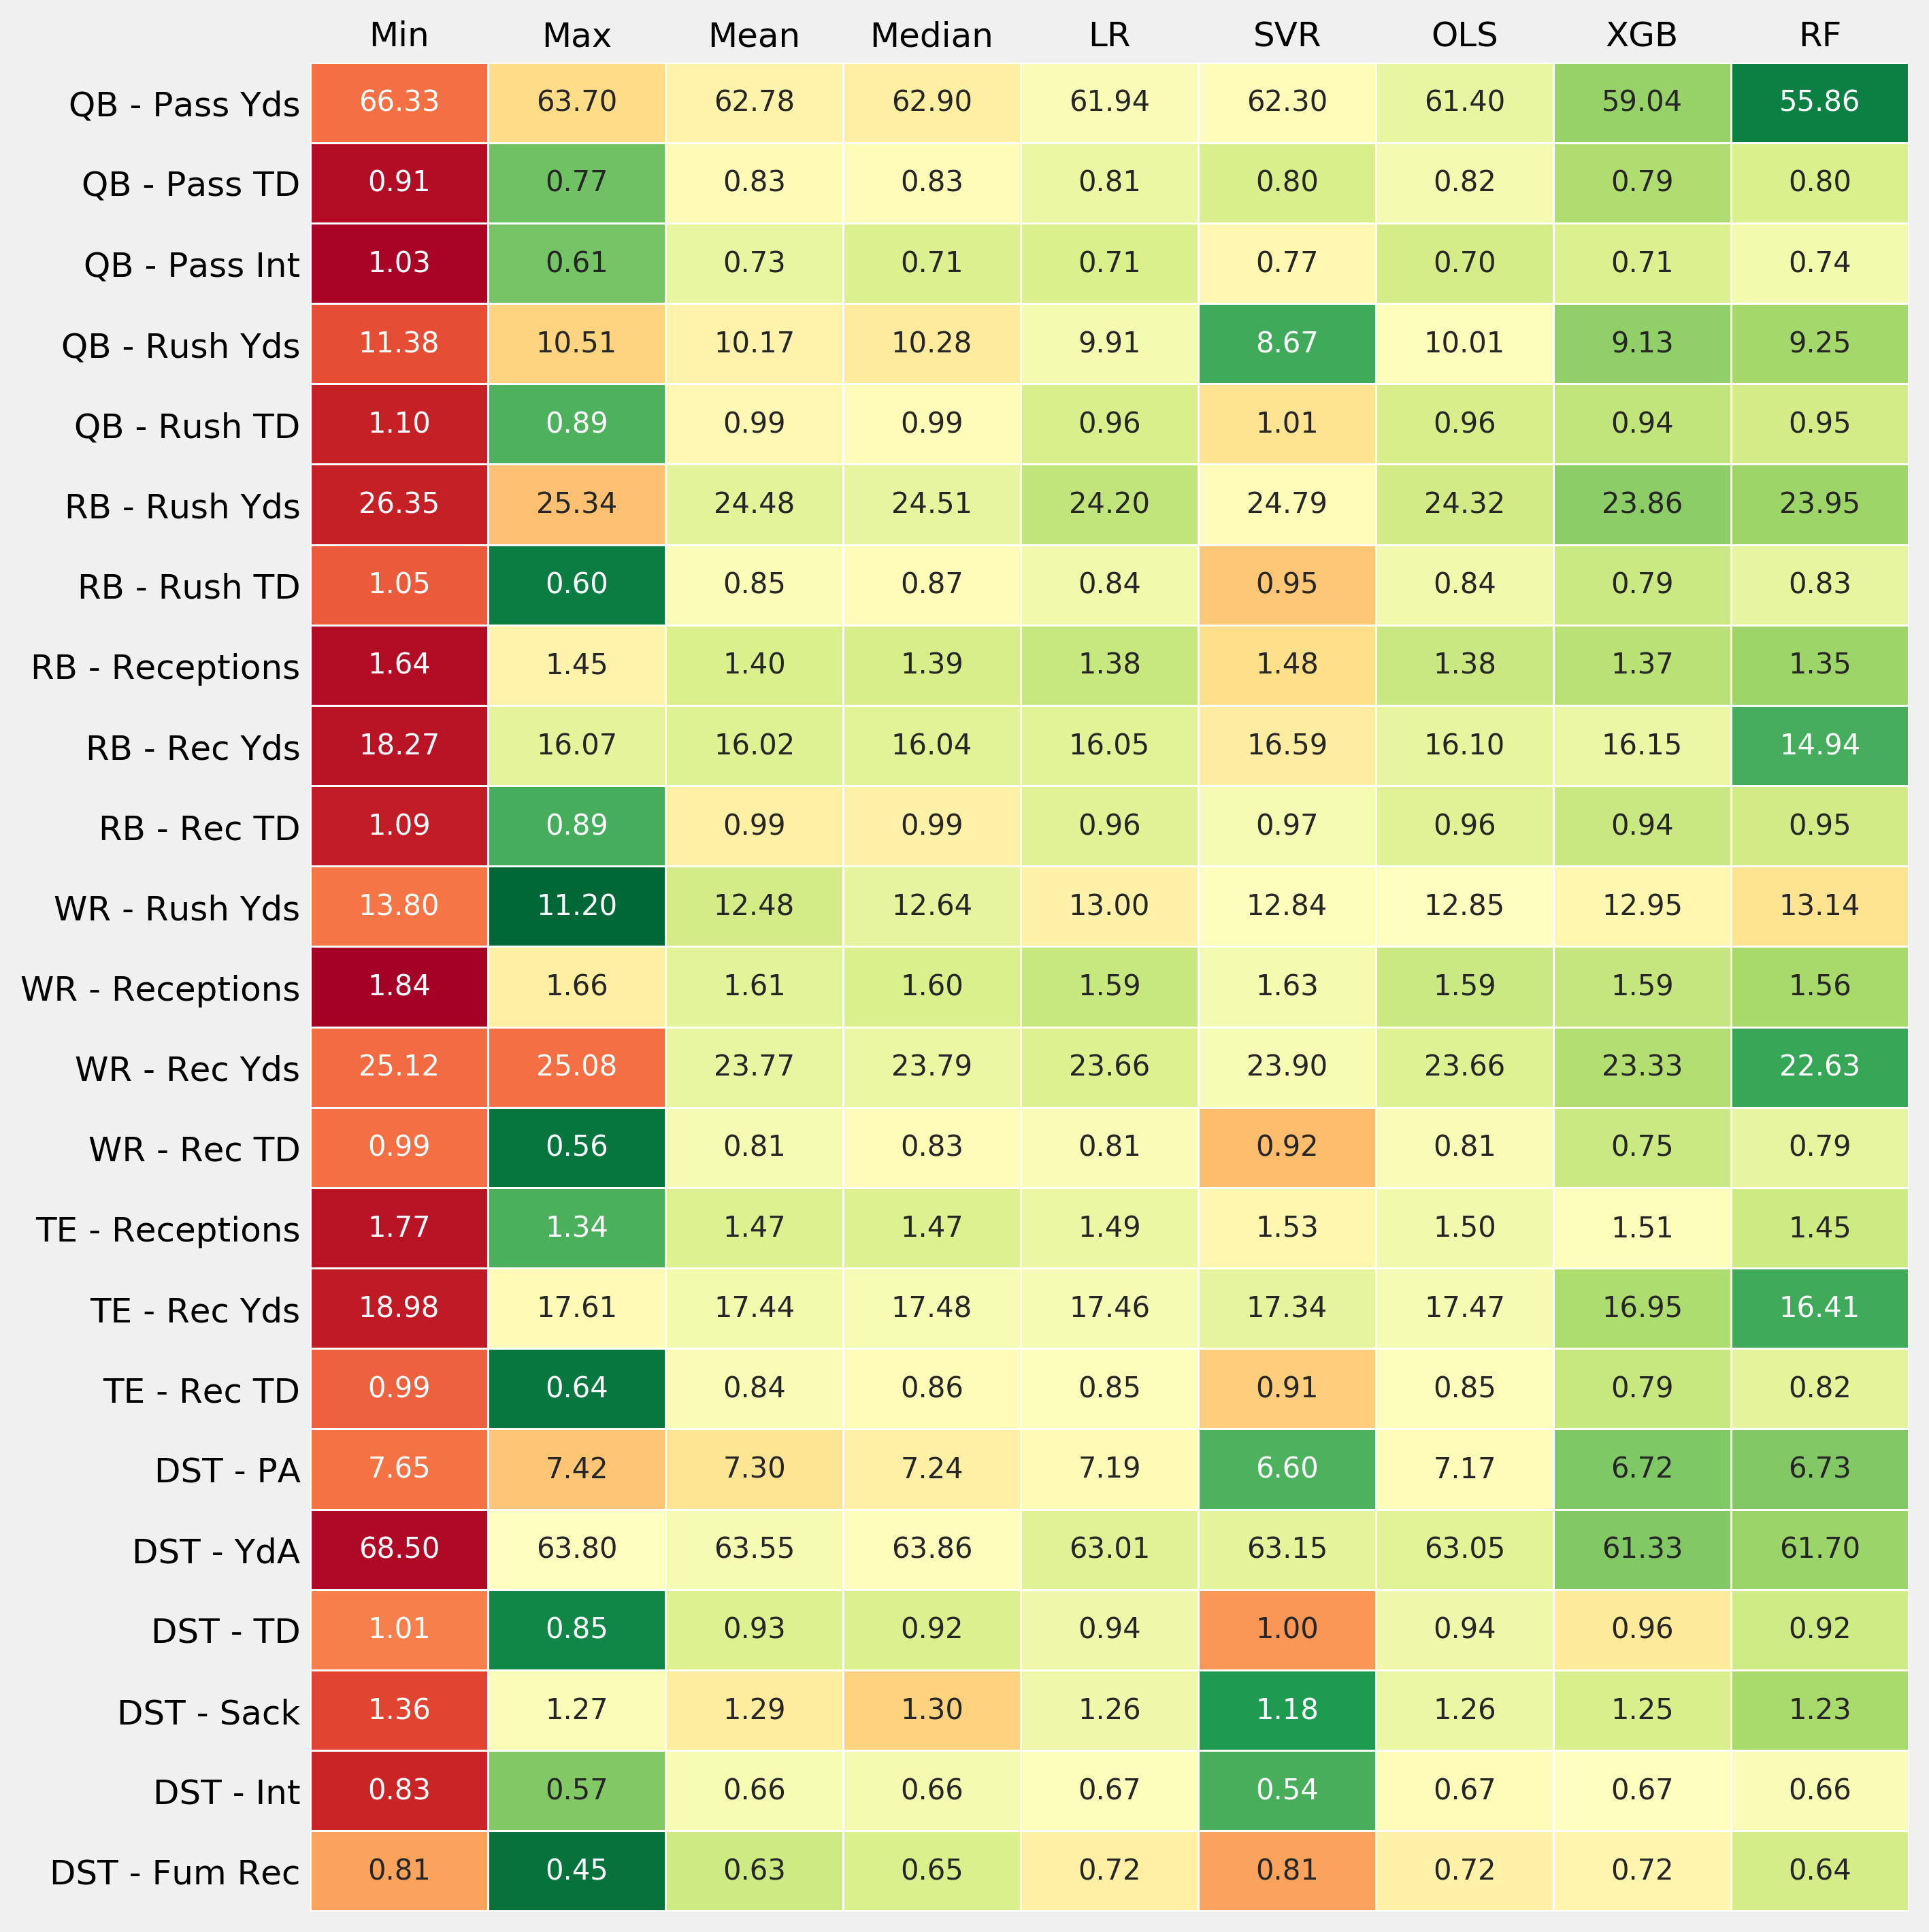
\includegraphics[width=1\textwidth]{../figures/essential_train_MAE_table}
    \caption{Training MAE.}
  \end{subfigure}
  \hfill
  \begin{subfigure}[b]{0.490\textwidth}
    \centering
    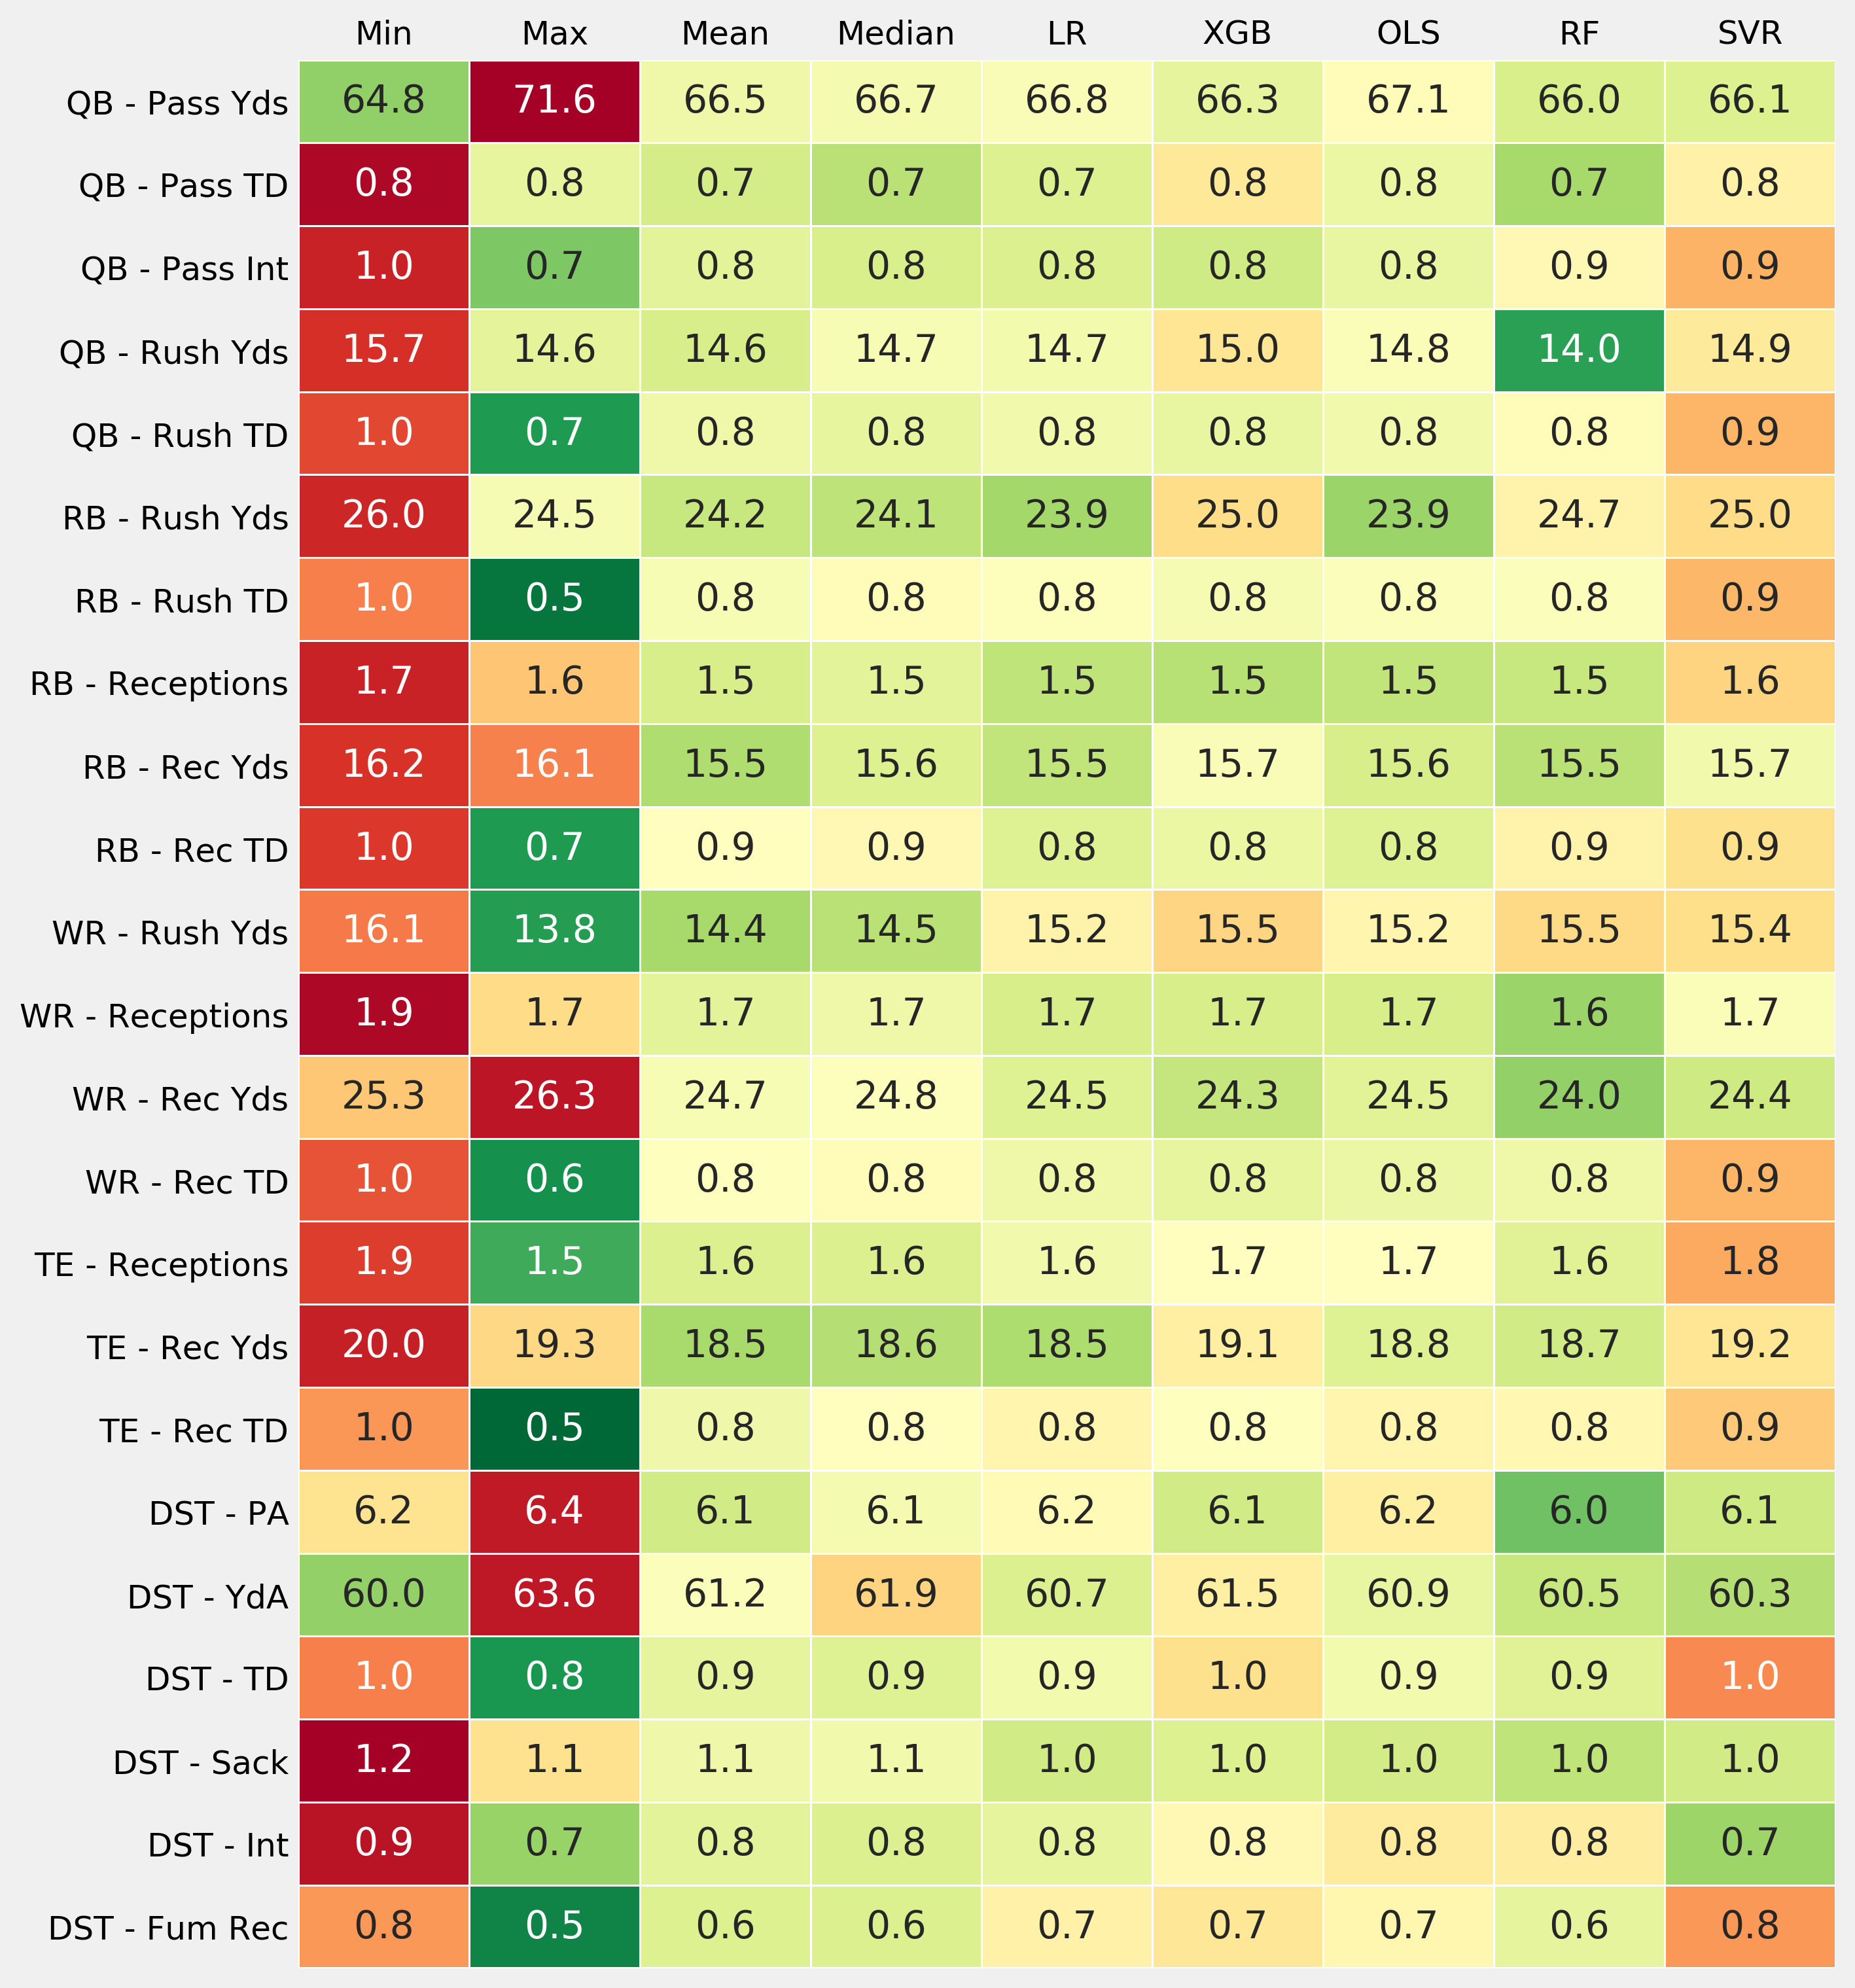
\includegraphics[width=1\textwidth]{../figures/essential_cv_MAE_table}
    \caption{Cross-Validation MAE.}
  \end{subfigure}
  \caption{Mean Absolute Error (MAE) values for all essential stats.}
  \label{train/cv MAE}
\end{figure}

Models with low MAE values on the training set but moderate to high MAE values on the cross-validation set indicate that the models overfit to the training set, and do not generalize well to unseen data. The optimal models for projecting each stat were manually chosen based on the MAE results from both the training and cross-validation sets. For stats such as DST - Fum Rec where both the cross-validation and training sets had the same optimal model (Max), that model was selected. For stats such as QB - Rush Yds, were the best model on the cross-validation set (RF) differed from the training set (SVR), the model performing best on the cross validation set was generally chosen. Some exceptions to these rules were made. For example, with QB Pass TD, although the RF slightly outperformed the Max on the cross-validation set, it significantly underperformed compared to Max on the training set. This indicates that the model may have gotten ``lucky'' on the cross-validation set and similar performance greater than the training set cannot be expected on new data. Additionally, when two models perform nearly equally well, a simpler model (Max) is preferable over a more complex model (RF). Hence, for QB - Pass TD Max was chosen as the projection function.\bigskip

Once the projection function was chosen for each stat, the test set data was loaded. Similar to the cross-validation set, the test set was scaled using the saved scaling data from the training set, and then the optimal projection function was applied to each stat, forming final projections for each stat and data that was completely unseen to models during hyperparameter tuning, and during the model selection process. As such, the test set provides a reliable estimate for the MAE expected for each stat on new data to the pipeline. The selected projection function for each stat, as well as its respective MAE value on the training, cross-validation, and test sets are provided in Table \ref{train/cv/test table}.



\begin{table}[H]
\caption{MAE values for training, cross-validation, and test sets with selected optimal projection function for each stat.}
\label{train/cv/test table}
\centering
\begin{tabular}{lllcrrr}
\toprule
{} & Position &        Stat & Projection Function &  Train &     CV &   Test \\
\midrule
{} &       QB &    Pass Yds &                  RF &  55.86 &  66.01 &  61.36 \\
{} &       {} &     Pass TD &                 Max &   0.77 &   0.75 &   0.79 \\
{} &       {} &    Pass Int &                 Max &   0.61 &   0.73 &   0.48 \\
{} &       {} &    Rush Yds &                  RF &   9.25 &  13.96 &  14.10 \\
{} &       {} &     Rush TD &                  RF &   0.95 &   0.83 &   1.12 \\
\midrule
{} &       RB &    Rush Yds &                 OLS &  24.32 &  23.90 &  23.51 \\
{} &       {} &     Rush TD &                 Max &   0.60 &   0.49 &   0.50 \\
{} &       {} &  Receptions &                 XGB &   1.37 &   1.50 &   1.27 \\
{} &       {} &     Rec Yds &                  RF &  14.94 &  15.48 &  14.08 \\
{} &       {} &      Rec TD &                 XGB &   0.94 &   0.85 &   0.89 \\
\midrule
{} &       WR &    Rush Yds &                 Max &  11.20 &  13.75 &  10.00 \\
{} &       {} &  Receptions &                  RF &   1.56 &   1.64 &   1.62 \\
{} &       {} &     Rec Yds &                  RF &  22.63 &  23.98 &  22.54 \\
{} &       {} &      Rec TD &                 Max &   0.56 &   0.58 &   0.59 \\
\midrule
{} &       TE &  Receptions &                 Max &   1.34 &   1.48 &   1.40 \\
{} &       {} &     Rec Yds &                  RF &  16.41 &  18.69 &  17.77 \\
{} &       {} &      Rec TD &                 Max &   0.64 &   0.53 &   0.80 \\
\midrule
{} &      DST &          PA &                  RF &   6.73 &   5.99 &   7.77 \\
{} &       {} &         YdA &                  RF &  61.70 &  60.50 &  55.52 \\
{} &       {} &          TD &                 Max &   0.85 &   0.84 &   0.73 \\
{} &       {} &        Sack &                 SVR &   1.18 &   1.04 &   1.12 \\
{} &       {} &         Int &                 SVR &   0.54 &   0.74 &   0.52 \\
{} &       {} &     Fum Rec &                 Max &   0.45 &   0.46 &   0.62 \\
\bottomrule
\end{tabular}
\end{table}

Several of the stats show some signs of difficulty to generalize to the new data. QB - Rush TD, TE - Rec TD, and DST - Fum Rec all had significantly higher test MAE values than their training and cross-validation counterparts. This could provide some future work as these models may require a closer look at data cleaning/thresholding, hyperparameter tuning, or model selection in order to better generalize. However, overall most stat projection test values were nearly equal to or better than their cross-validation MAE value, showing the ability for most models to generalize well to unseen data.\bigskip

Interestingly, a simple maximum was the most frequent model selection, followed by a random forest, though all machine learning models were utilized for at least one stat. This indicates the largest differences in projecting different stats for different positions. For example, Rush Yds were found to be optimally projected using RF, OLS, and simple Max for QB, RB, and WR respectively, indicating that the algorithms used by each source are different depending upon not only stat but also position.\bigskip

TODO: talk about applying scoring rules and floor ceiling projections.\bigskip


Once final projections are computed using scoring rules, the projections for any position can be visualized. Figure \ref{qb17} displays an example visualization for quarterbacks in week 17 scored by FanDuel. In addition to simply showing the generated projections, confidence intervals of each player's respective floor and ceiling are included as well as player status. Statuses include Q for questionable, IR for players on injured reserved, SSPD for suspended players, and O for players who are out.

\begin{figure}[H]
  \centering
  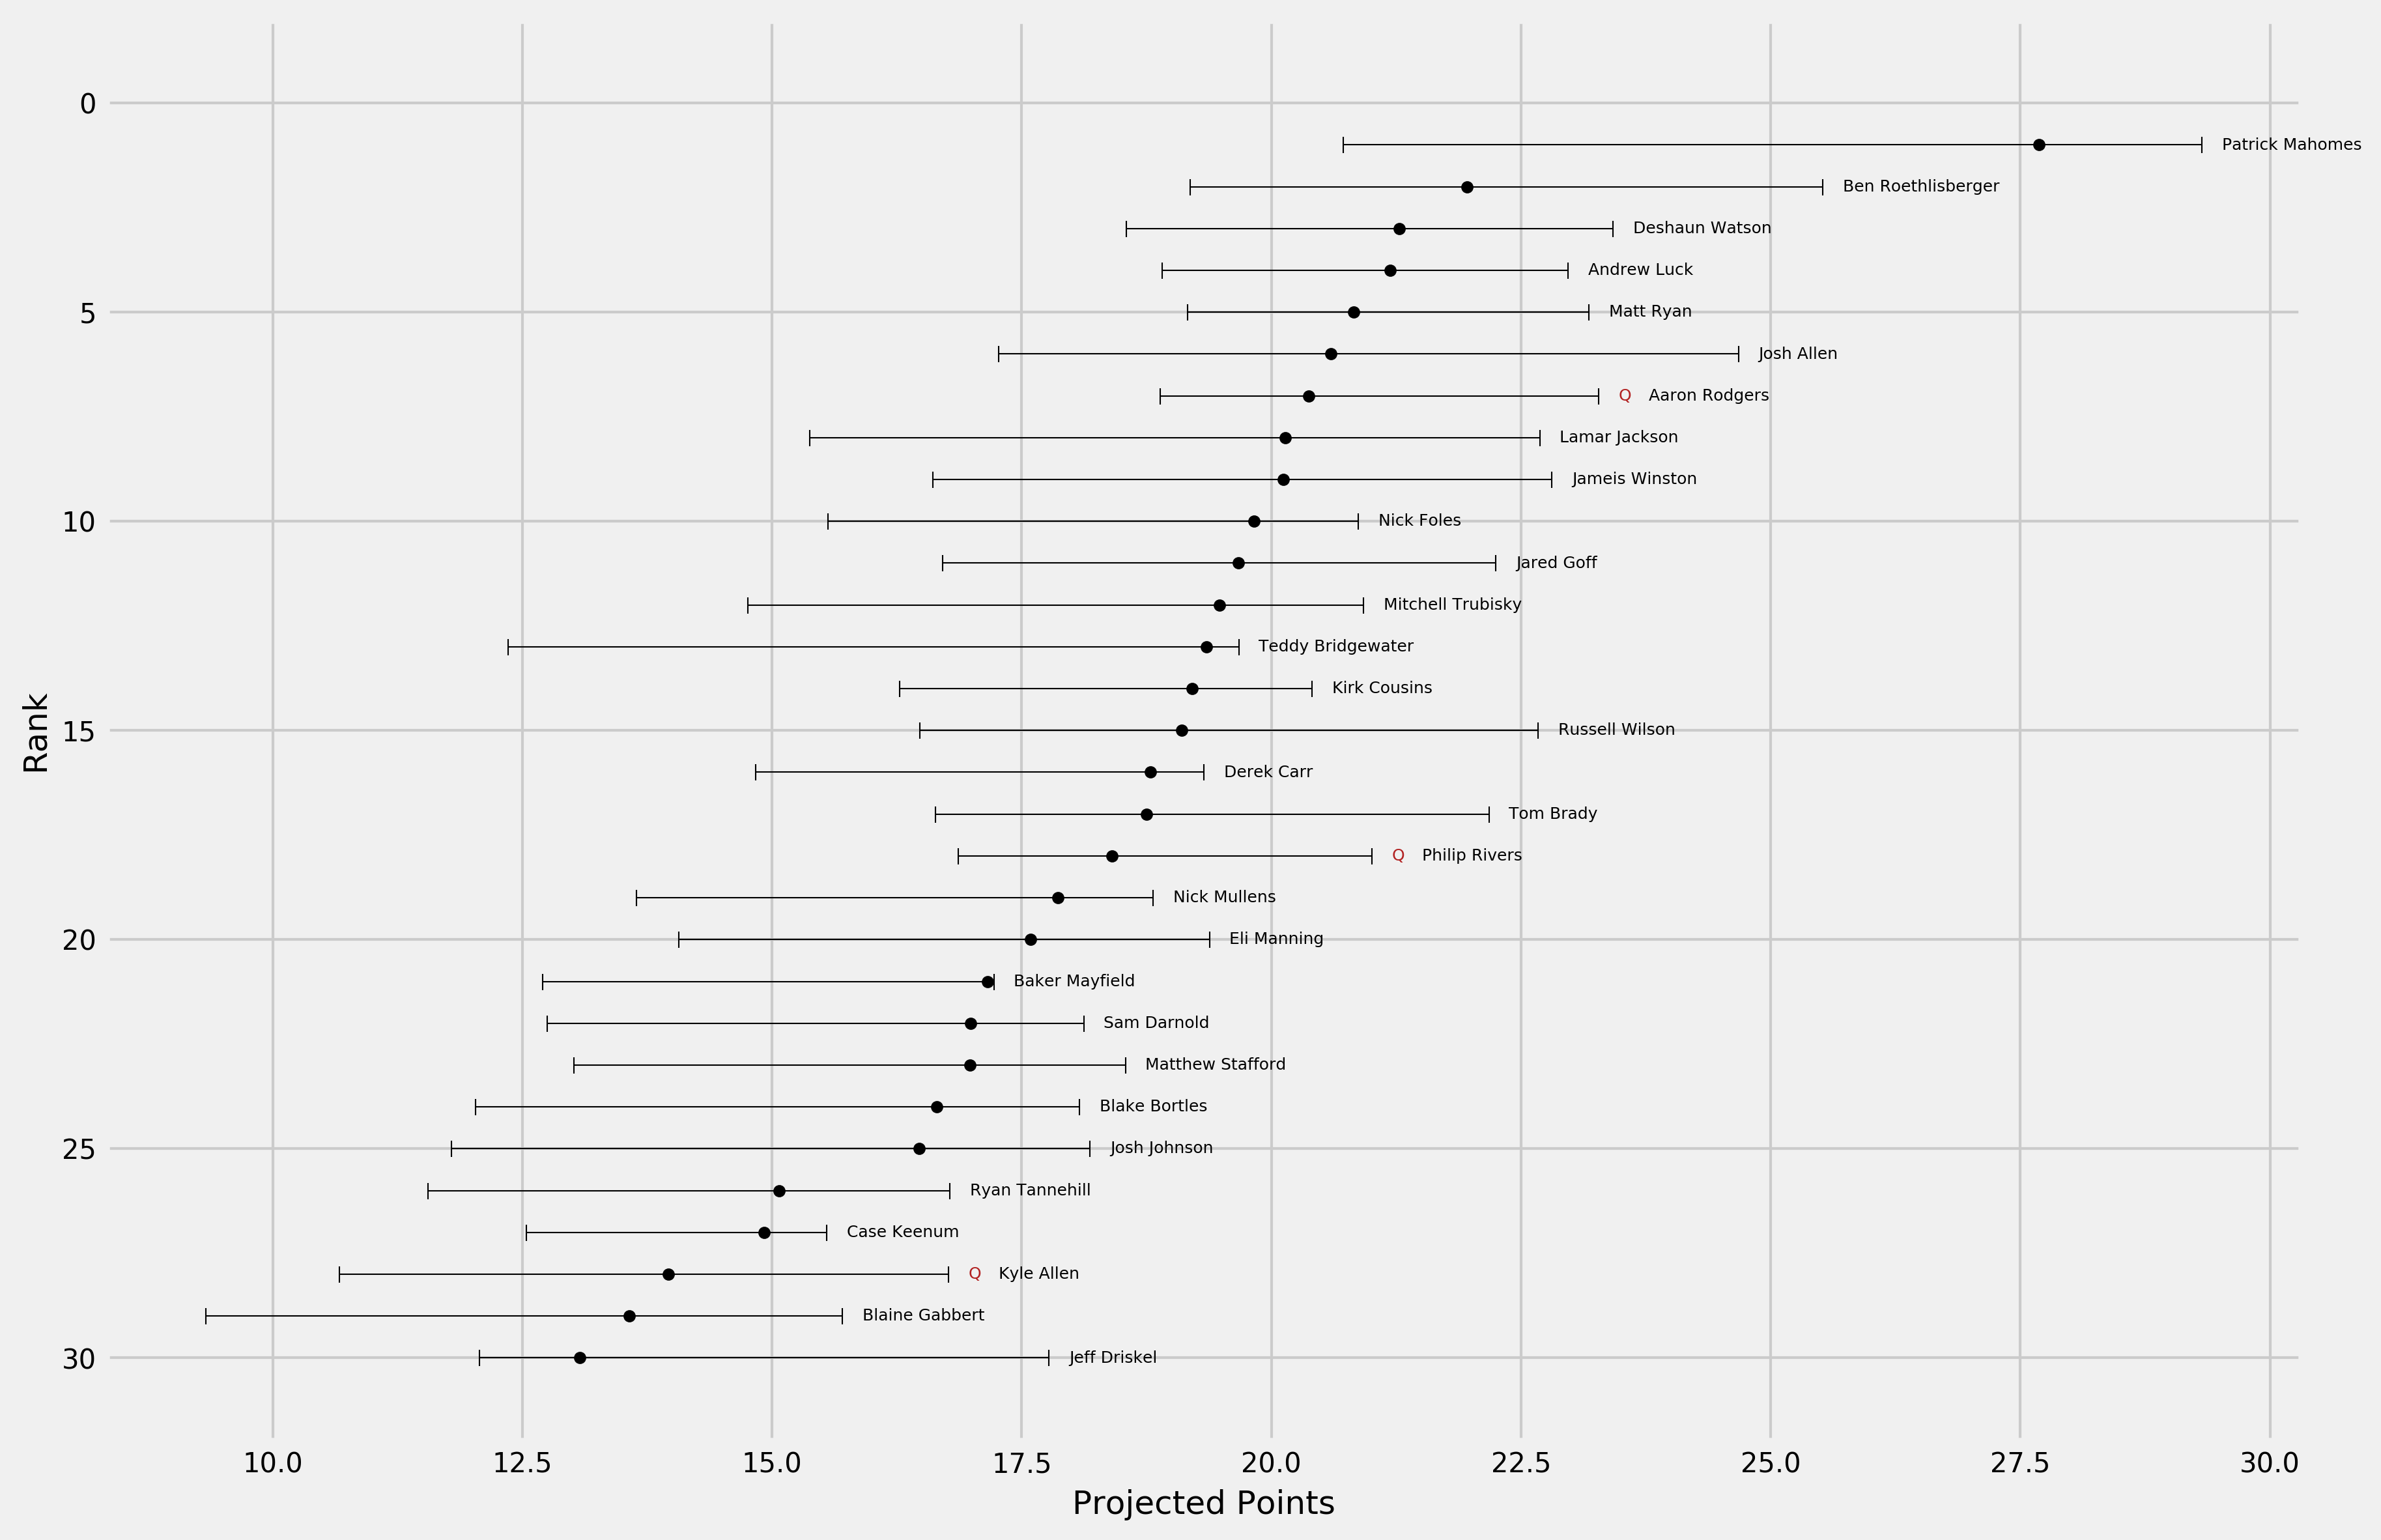
\includegraphics[width=0.95\textwidth]{../figures/QB_17}
  \caption{Example projections for QB week 17. Dots indicate the projections generated using our methodology, with error bars representing total floor and total ceiling for each player. Red text indicates the status of players.}
  \label{qb17}
\end{figure}


\subsection{Lineup Optimization}
Given optimal player projections, lineups must now be generated for competition at DraftKings and FanDuel. Both sites have the same lineup restrictions, only differing on their budget and point system (DraftKings is 50,000 budget and 1 pt per reception; FanDuel is 60,000 budget and is 0.5 pts per reception). As the goal is to score as many points as possible, projected points were maximized such that all lineup restrictions were met. \bigskip

In order to use convex optimization to solve for the optimal lineup, as opposed to brute-force solving for all possible combinations, we define the following problem: \begin{itemize}
	\item Let $N$ be the number of total players.
	\item Let $B$ be the salary budget for the contest.
	\item Let $w \in \mathbb{R}^{N}$ be a vector of player-weights, such that $w_i \in {0, 1}$.
	\item Let $P \in \mathbb{R}^{N}$ be a vector of projected points.
	\item Let $S \in \mathbb{R}^{N}$ be a vector of salaries.
	\item Let $D \in \mathbb{R}^{N \times 5}$ be a matrix containing the position of  each player, using dummy variables for each position. That is, $p_{i, j} \in {0, 1}$.
	\item Let $C \in \mathbb{R}^{N \times 32}$ be a matrix containing the team of each player, using dummy variables for each team. That is, $T_{i, j} \in {0, 1}$.
\end{itemize}
Then, we solve for the $w$ that solves:
\begin{equation*}
\begin{aligned}
& \underset{w}{\text{maximize}}
& & w^T \cdot P \\
& \text{subject to}
& & w^T \cdot S \leq B, \; \mathds{1} \cdot w = 9, \\
&&& (w^T \cdot D)_1 = 1, \\
&&& 2 \leq (w^T \cdot D)_2 \leq 3, \\
&&& 3 \leq (w^T \cdot D)_3 \leq 4, \\
&&& 1 \leq (w^T \cdot D)_4 \leq 2, \\
&&& (w^T \cdot D)_5 = 1, \\ 
&&& \max_i (w^T \cdot C)_i \leq 4 \\
\end{aligned}
\end{equation*}
where the subscripts $1,\ldots ,5$ on $(w^T \cdot D)$ correspond to the positions QB, RB, WR, TE, and Defense, respectively. These constraints ensure that each lineup follows the composition rules defined in each contest.

While this formulation worked perfectly when solving for the highest projected lineup, it failed when scaling to the solve for the highest $n$ projected lineups. As many contests allow for up to 150 lineup entries per person, this limitation must be solved for. Below in figure \ref{lineup times}, the exponential nature of the slowdown is shown.

\begin{figure}[H]
  \centering
  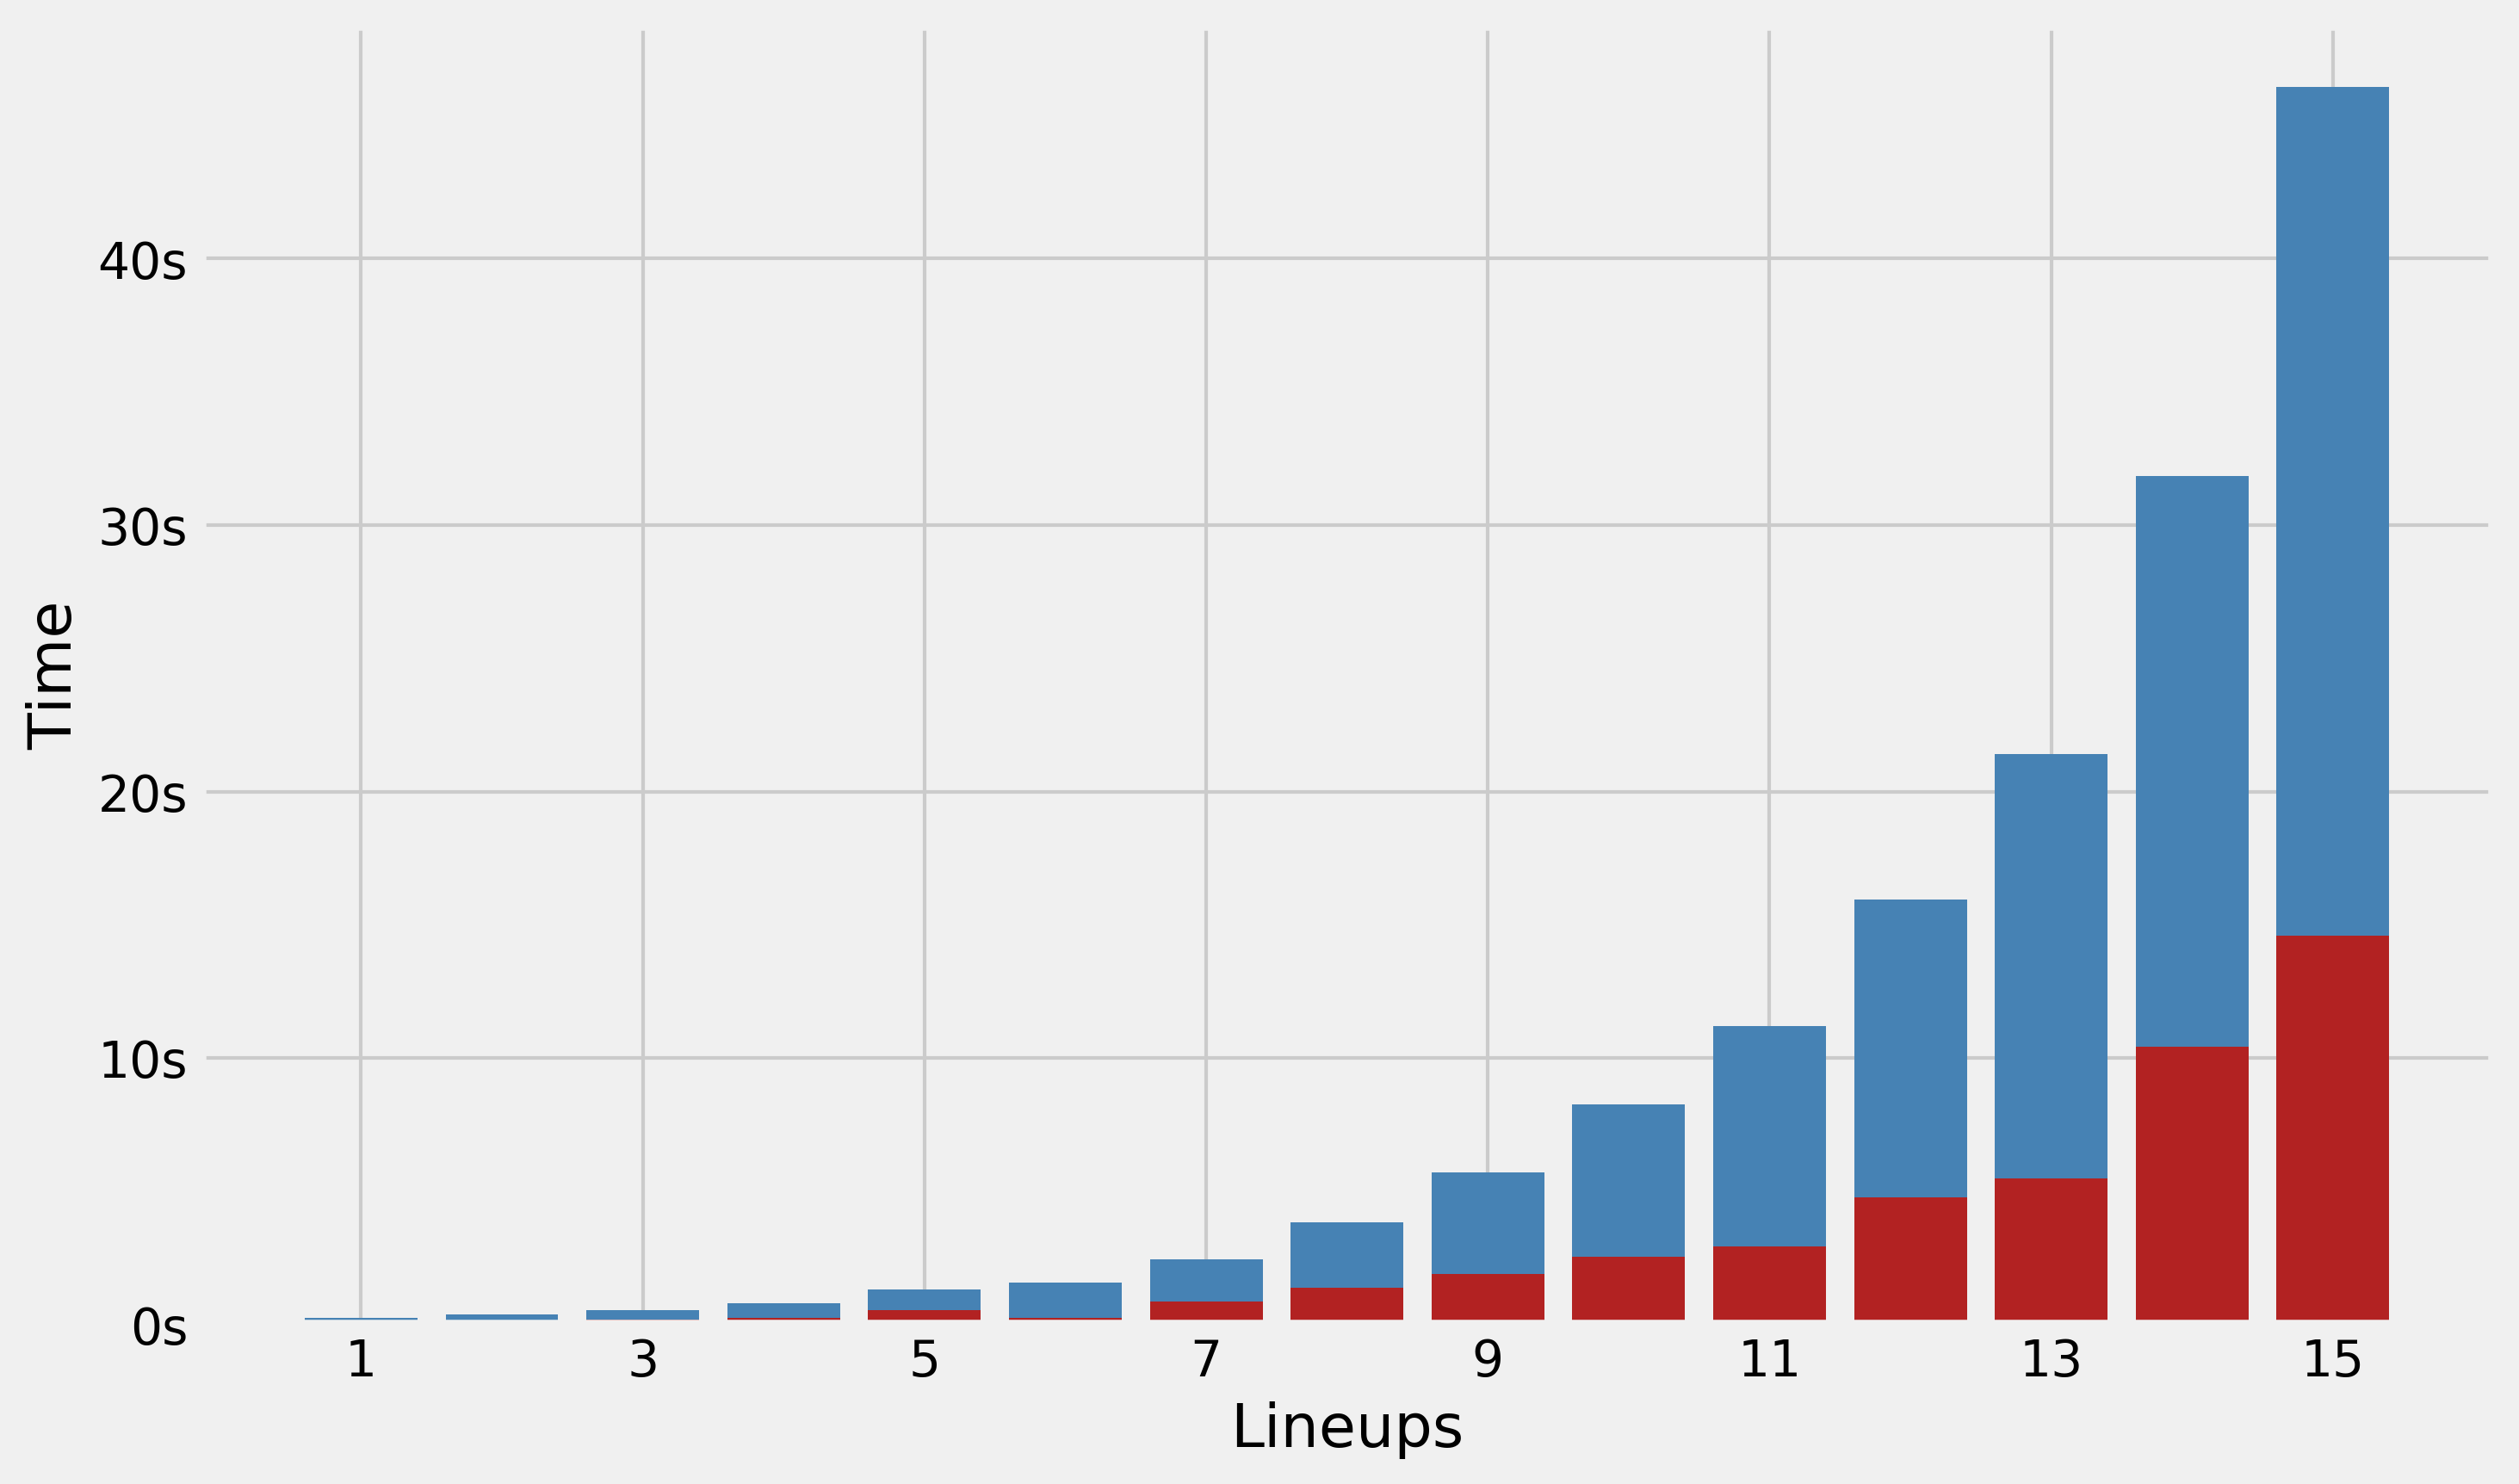
\includegraphics[width=0.95\textwidth]{../figures/time_per_lineup}
  \caption{Cumulative (in blue) and marginal (in red) time taken to generate lineups.}
  \label{lineup times}
\end{figure}

As a remedy for this problem, we implement a dropout-like system in which players are dropped from the available pool with probability $p$ (CITE). Thus, the probability that the best possible lineup gets chosen is equal to $(1-p)^9$. Below in Table \ref{probs_of_lineups}, these probabilities are shown for different values of $p$.

\begin{table}[H]
\caption{Probability of best lineup being selected for varying levels of dropout probability $p$.}
\label{probs_of_lineups}
\centering
\begin{tabular}{lcc}
\toprule
{} &     $p$ &  $\Pr$(Max)  \\
\midrule
{} &  0.00 &  1.00 \\
{} &  0.05 &  0.63 \\
{} &  0.10 &  0.39 \\
{} &  0.15 &  0.23 \\
{} &  0.20 &  0.13 \\
{} &  0.25 &  0.08 \\
{} &  0.30 &  0.04 \\
{} &  0.35 &  0.02 \\
{} &  0.40 &  0.01 \\
\bottomrule
\end{tabular}
\end{table}

Now of course, for what this approach gains in speed, it loses in precision. We have now introduced a non-zero probability that the best possible $n$ lineups will not be selected if we choose to generate exactly $n$ lineups, given the randomness of dropout. Using week 1 of 2018 as a test, 400 lineups were generated, and the first $n$ lineups generated are examined below in Figure \ref{lineups_vs_n}. Both the top 10 and top 150 lineups are studied.  

\begin{figure}[H]
  \centering
  \begin{subfigure}[b]{0.80\textwidth}
    \centering
    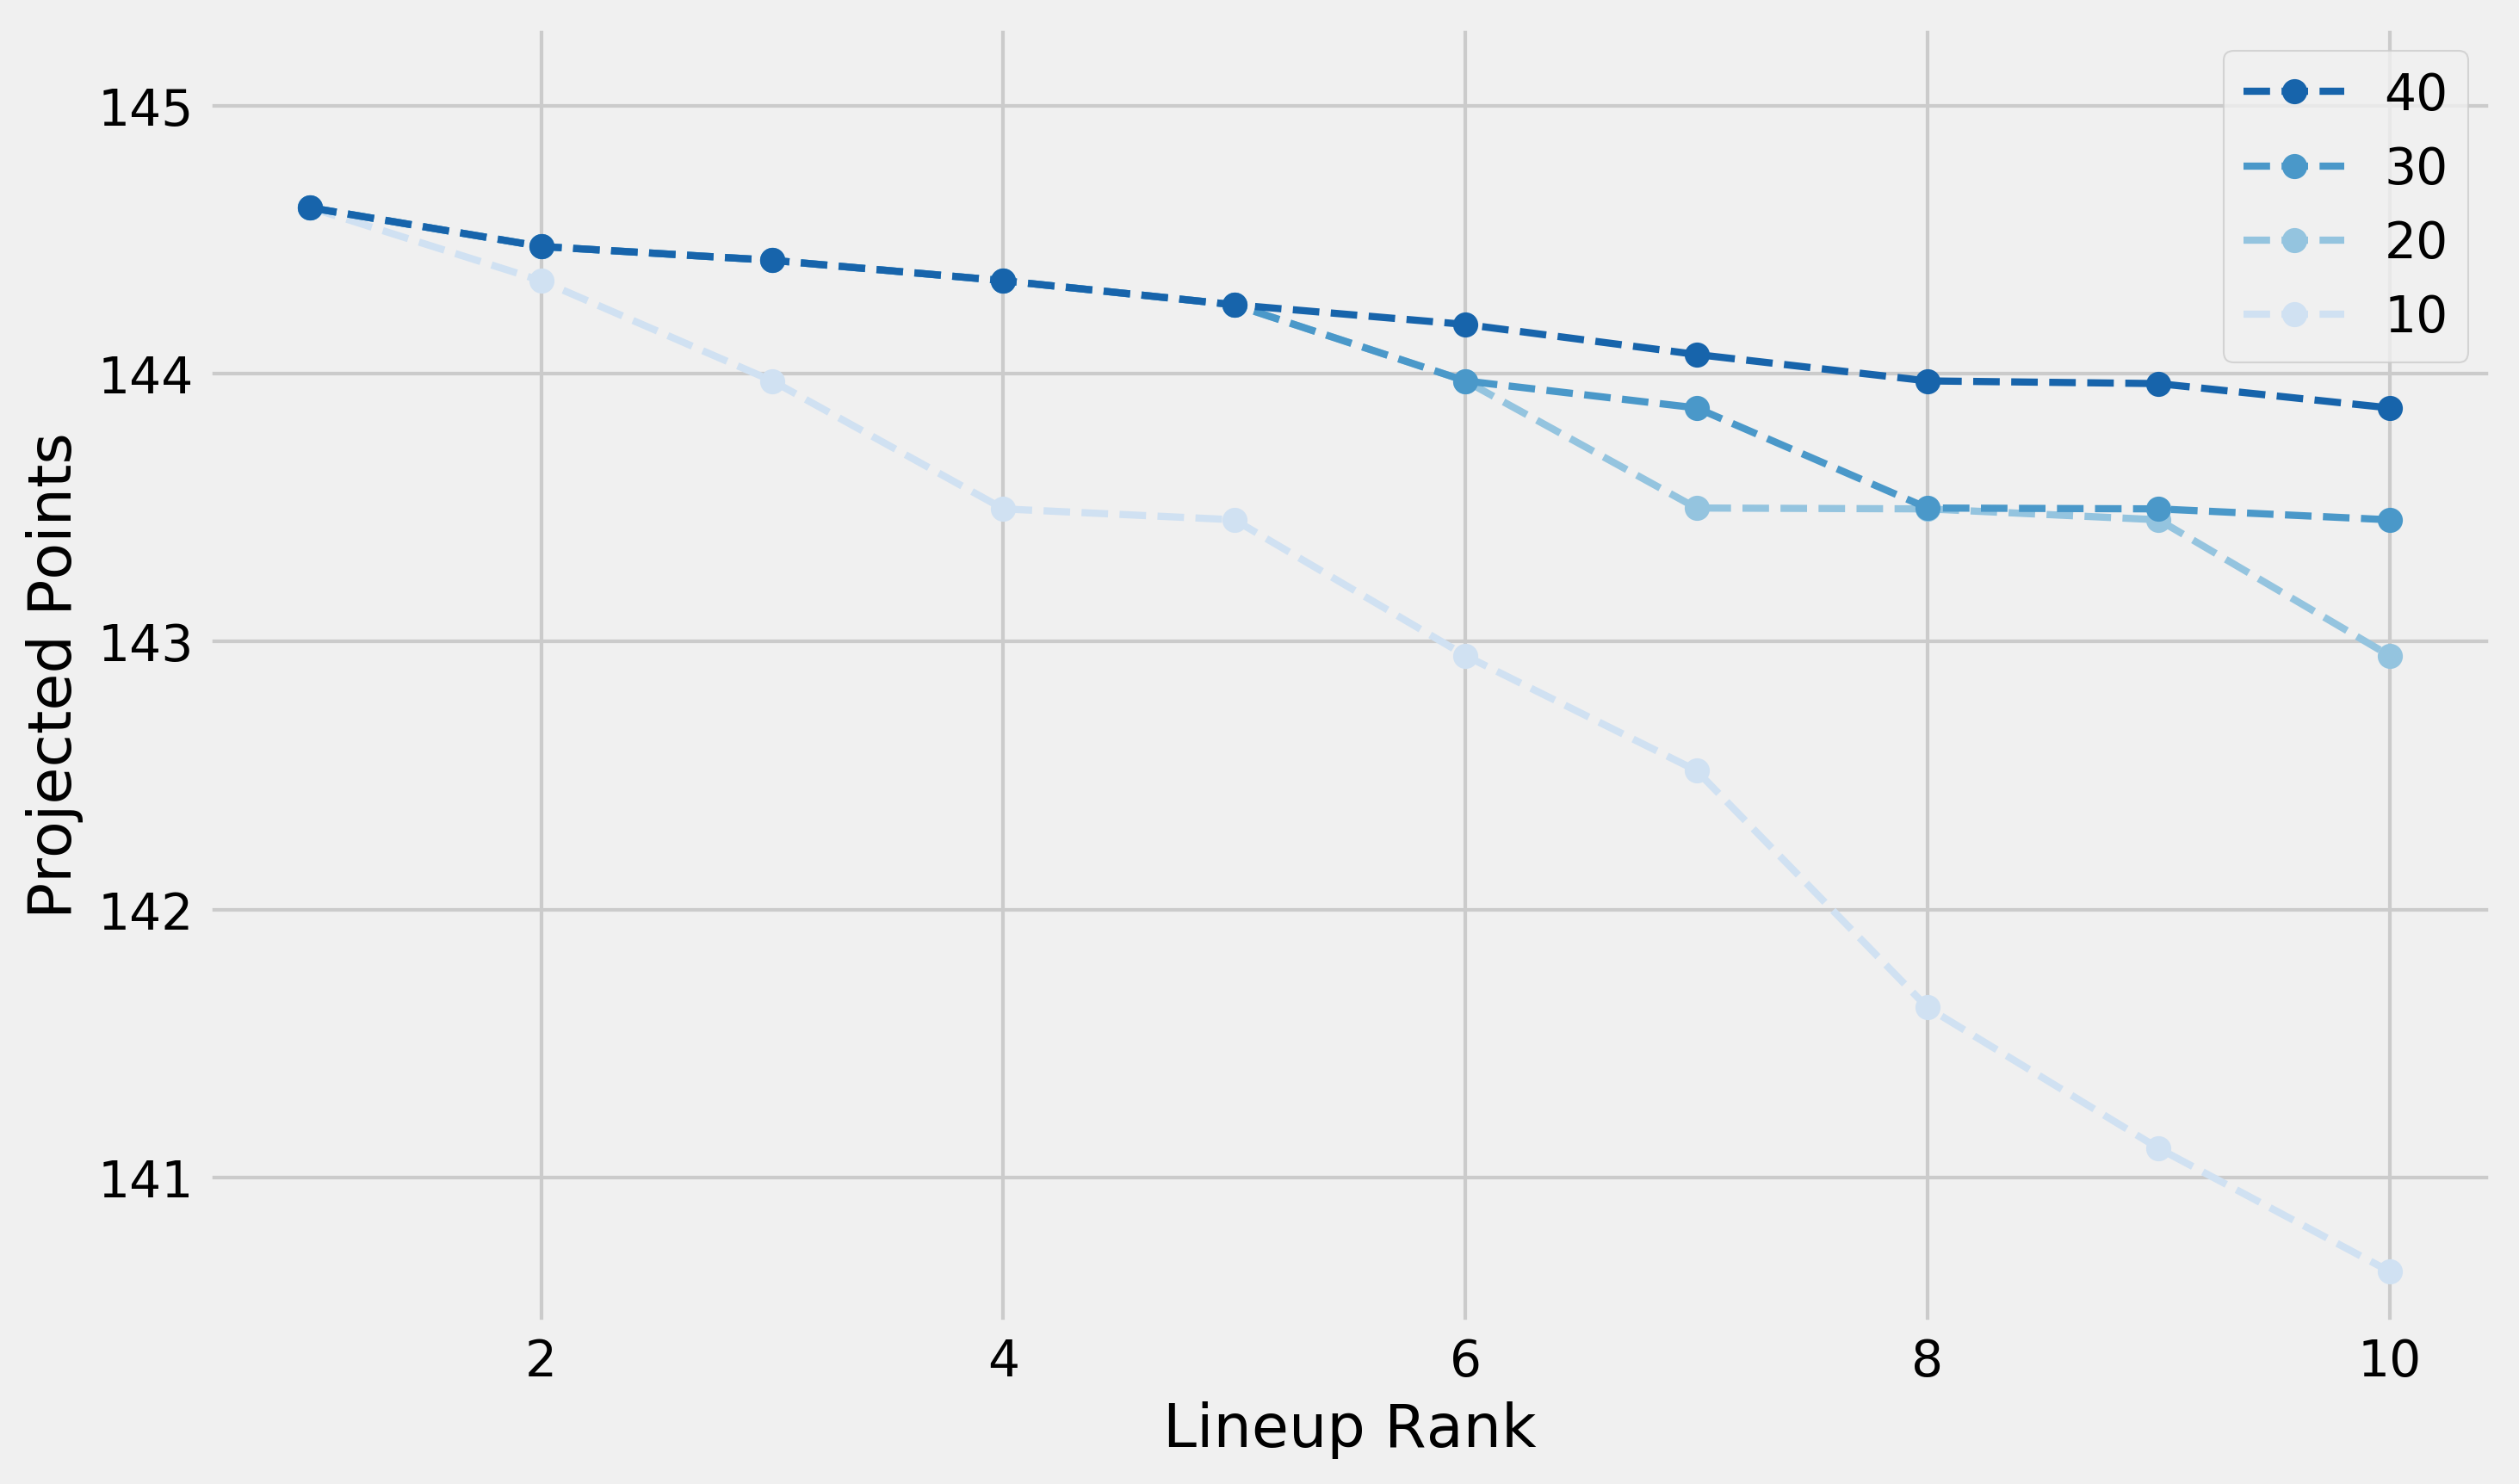
\includegraphics[width=1\textwidth]{../figures/lineups10_vs_n}
    \caption{Top 10 lineups.}
  \end{subfigure}
  \par\bigskip
  \begin{subfigure}[b]{0.80\textwidth}
    \centering
    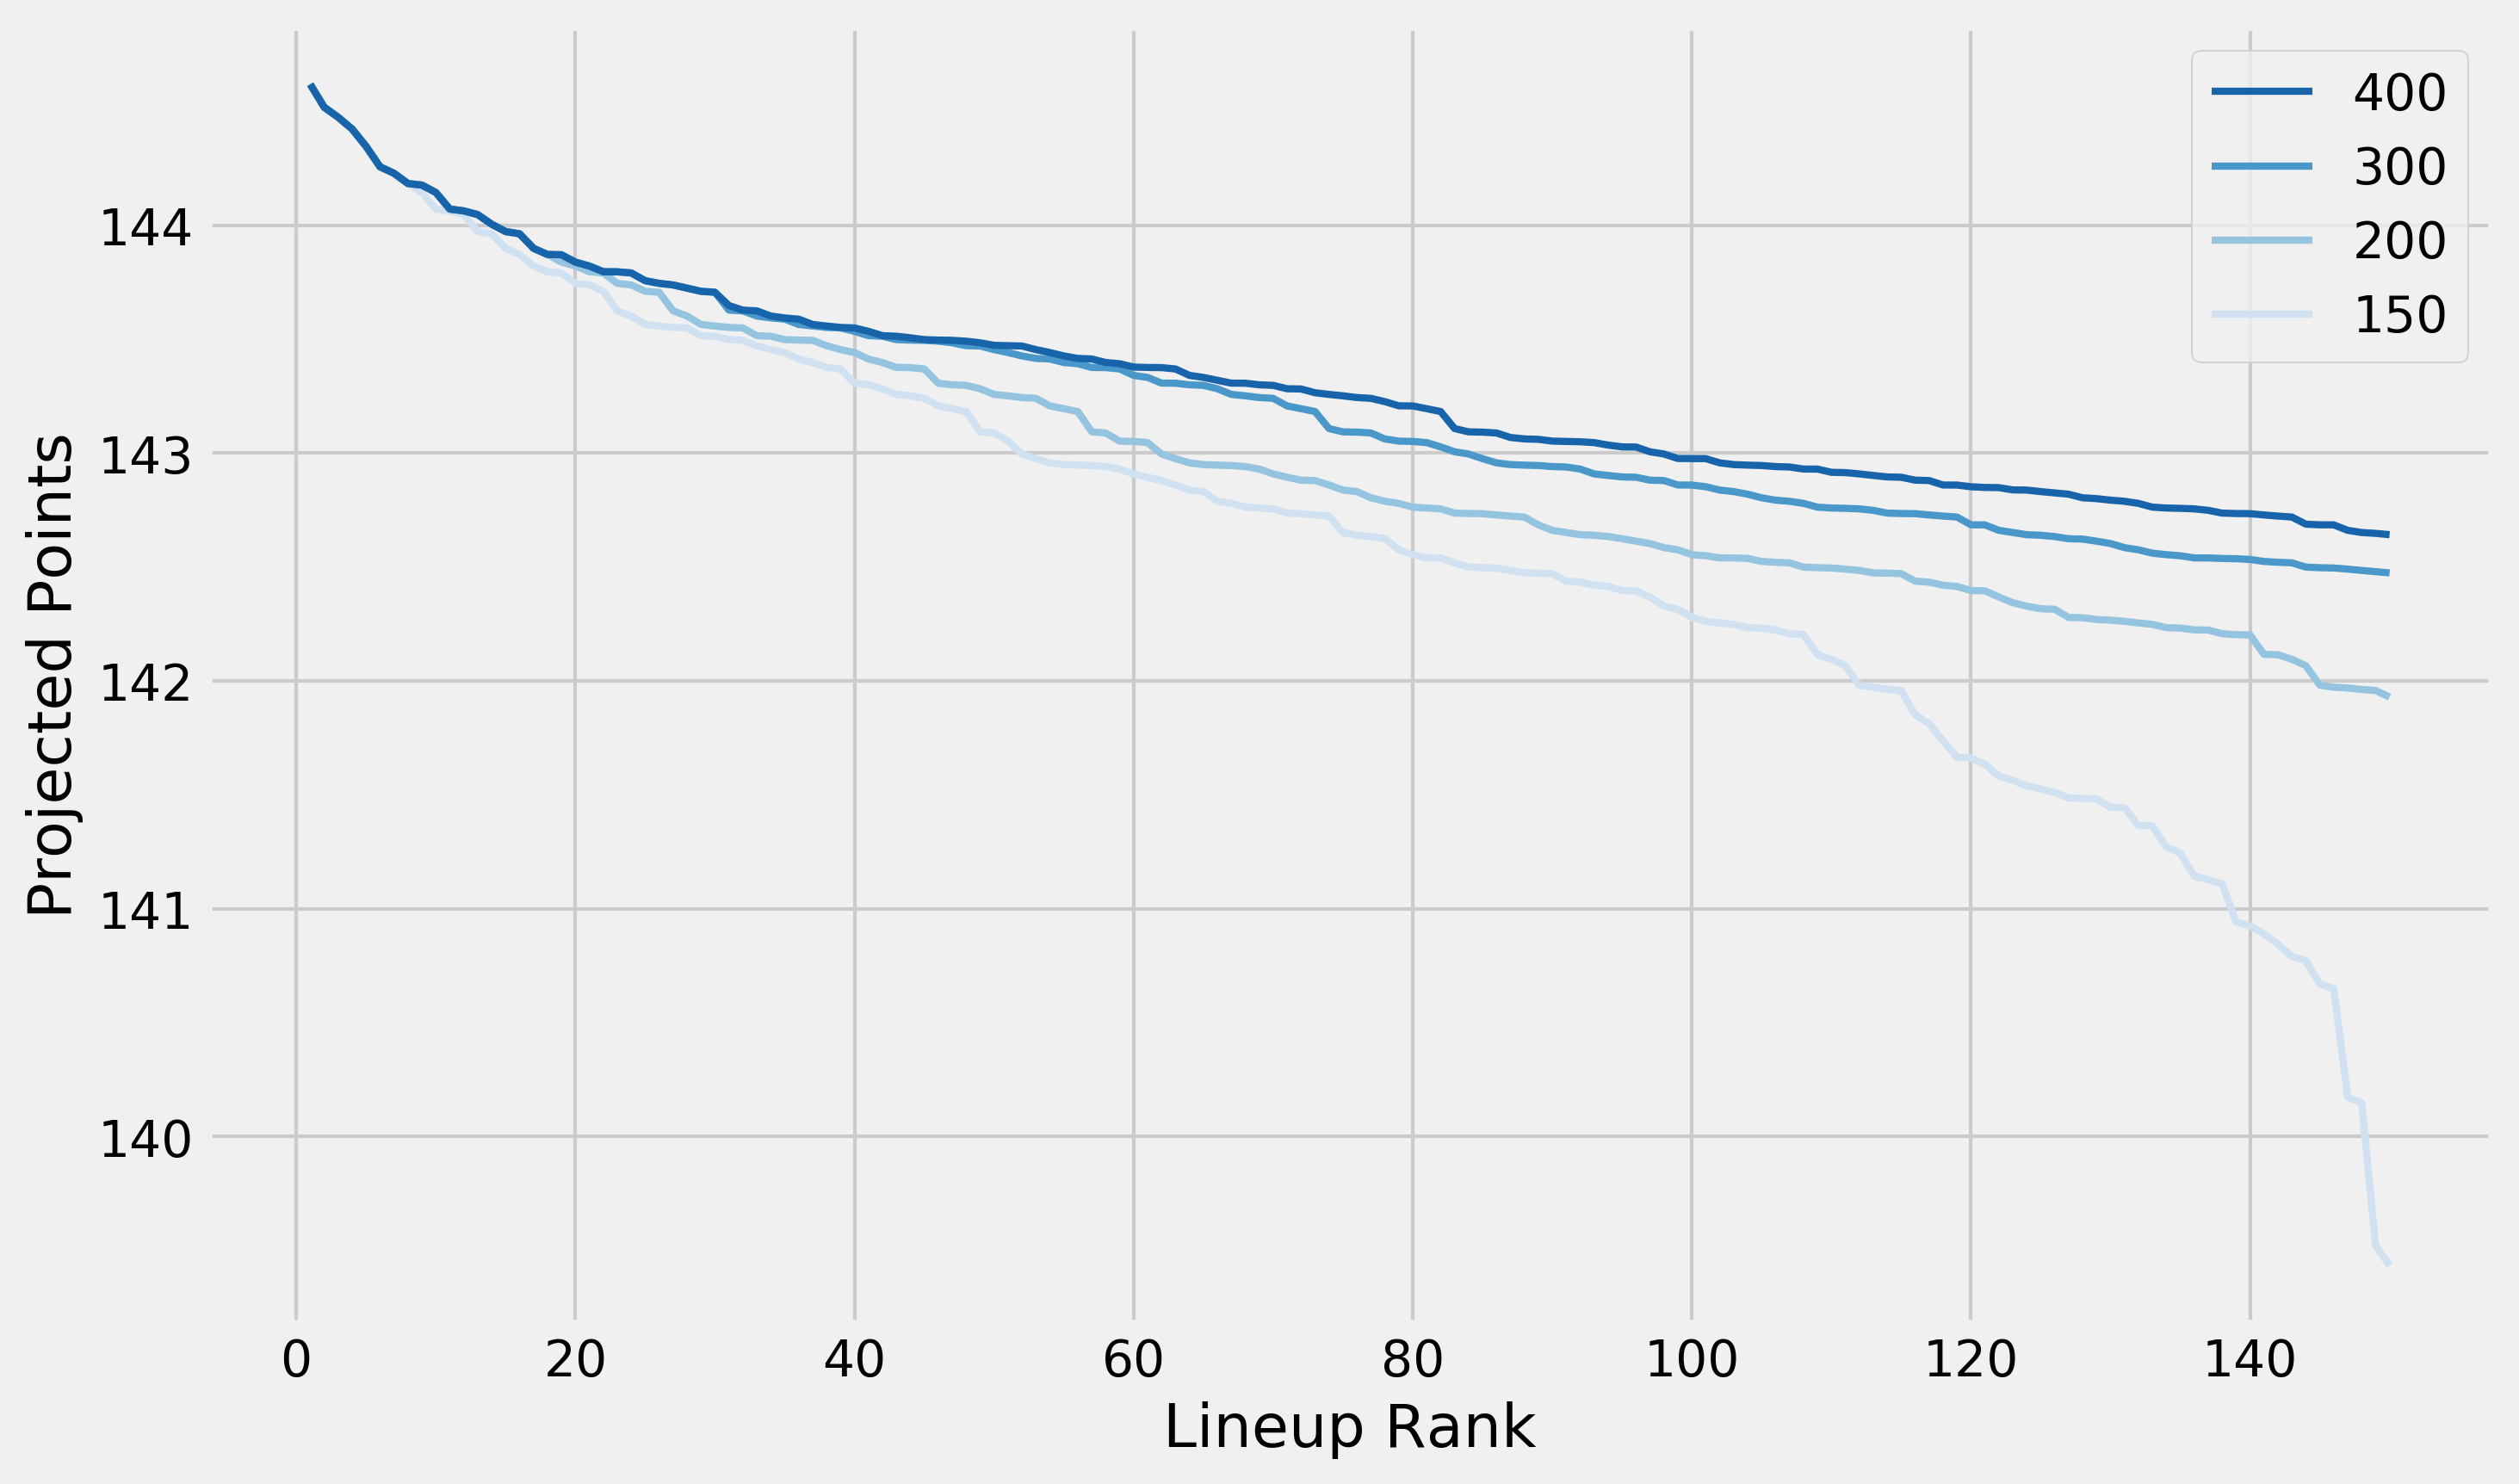
\includegraphics[width=1\textwidth]{../figures/lineups150_vs_n}
    \caption{Top 150 lineups.}
  \end{subfigure}
  \caption{Projected points are plotted against lineup rank for the first $n$ lineups generated.}
\label{lineups_vs_n}
\end{figure}

From Figure \ref{lineups_vs_n}, it is clear that if $n$ lineups are needed, naively choosing $n$ lineups to generate will produce a sub-optimal output.

\pagebreak
\section{Results}


TODO



\pagebreak
\section{Future Work}
Future work may consist of several improvements to the described methodology. First, more data from other sources may be incorporated. Many additional sources provide similar projections on a weekly basis, but do not store historical projections online. These sources can be scraped each week during the season in order to keep a private history to use for model building. Additionally, several sources are behind paywalls, so paid membership accounts can be created to include them. The law of big data in machine learning states that more data can only result in more accurate predictions, thus including more sources should only improve the projections generated.\bigskip

Second, several models did not generalize well to the test set. Modulating threshold values and hyperparameter grids may help overcome these issues. Additionally, including other machine learning algorithms such as neural networks may further improve accuracy and precision of generated projections.\bigskip

Finally, during lineup creation, simple linear interpolation between the floor, generated projection, and ceiling are used to create 150 lineups. Using the floor and ceiling levels to instead create a distribution with mode or mean equal to the generated projection and performing Monte Carlo simulations to generate lineups may further improve the ability to generate profitable lineups.

\section{Conclusion}
TODO: conclusions

% ------------------------------------ References ---------------------------------------------- %

\pagebreak
\begin{thebibliography}{}

\bibitem{fancyimpute}
A. Rubinsteyn, \& S. Feldman (2019). 
``A Variety of Matrix Completion and Imputation Algorithms Implemented in Python.'' 
\url{https://github.com/iskandr/fancyimpute}

\bibitem{LR paper}
H. Zhou \& T. Hastie (2005). 
``Regularization and Variable Selection via the Elastic Net.'' 
\textit{R. Statist. Soc.B,} 67, 301–32

\bibitem{LR algo}
M. Brucher et. al (2019). 
ElasticNet. \url{https://scikit-learn.org/stable/modules/generated/sklearn.linear_model.ElasticNet.html}

\bibitem{XGB paper}
T. Chen \& C. Guestrin (2016). 
``XGBoost: A Scalable Tree Boosting System.'' 
\textit{Proceedings of the 22Nd ACM SIGKDD International Conference on Knowledge Discovery and Data Mining,} 785-794

\bibitem{XGB algo}
T. Chen et. al (2019). 
XGBoost. \url{https://xgboost.readthedocs.io/en/latest/python/index.html}

\bibitem{OLS algo}
S. Seabold et. al (2019). 
OLS. \url{https://www.statsmodels.org/dev/generated/statsmodels.regression.linear_model.OLS.html}

\bibitem{RF paper}
A. Liaw \& M. Wiener (2002). 
``Classificationand RegressionbyrandomForest.'' 
\textit{R News,} 2/3:18-22

\bibitem{RF algo}
M. Brucher et. al (2019). 
RandomForestRegressor. \url{https://scikit-learn.org/stable/modules/generated/sklearn.ensemble.RandomForestRegressor.html}

\bibitem{SVR paper}
H. Drucker, C.J.C. Burges, L. Kaufman, A. Smola, \& V. Vapnik (1997).
``Support Vector Regression Machines.'' 
\textit{Advances in Neural Information Processing Systems,} 9, 155–161

\bibitem{SVR algo}
M. Brucher et. al (2019). 
SVR. \url{https://scikit-learn.org/stable/modules/generated/sklearn.svm.SVR.html}



\end{thebibliography}

\pagebreak
\section{Appendix}
\subsection{Nonessential Stats Summary}

\begin{figure}[H]
  \centering
  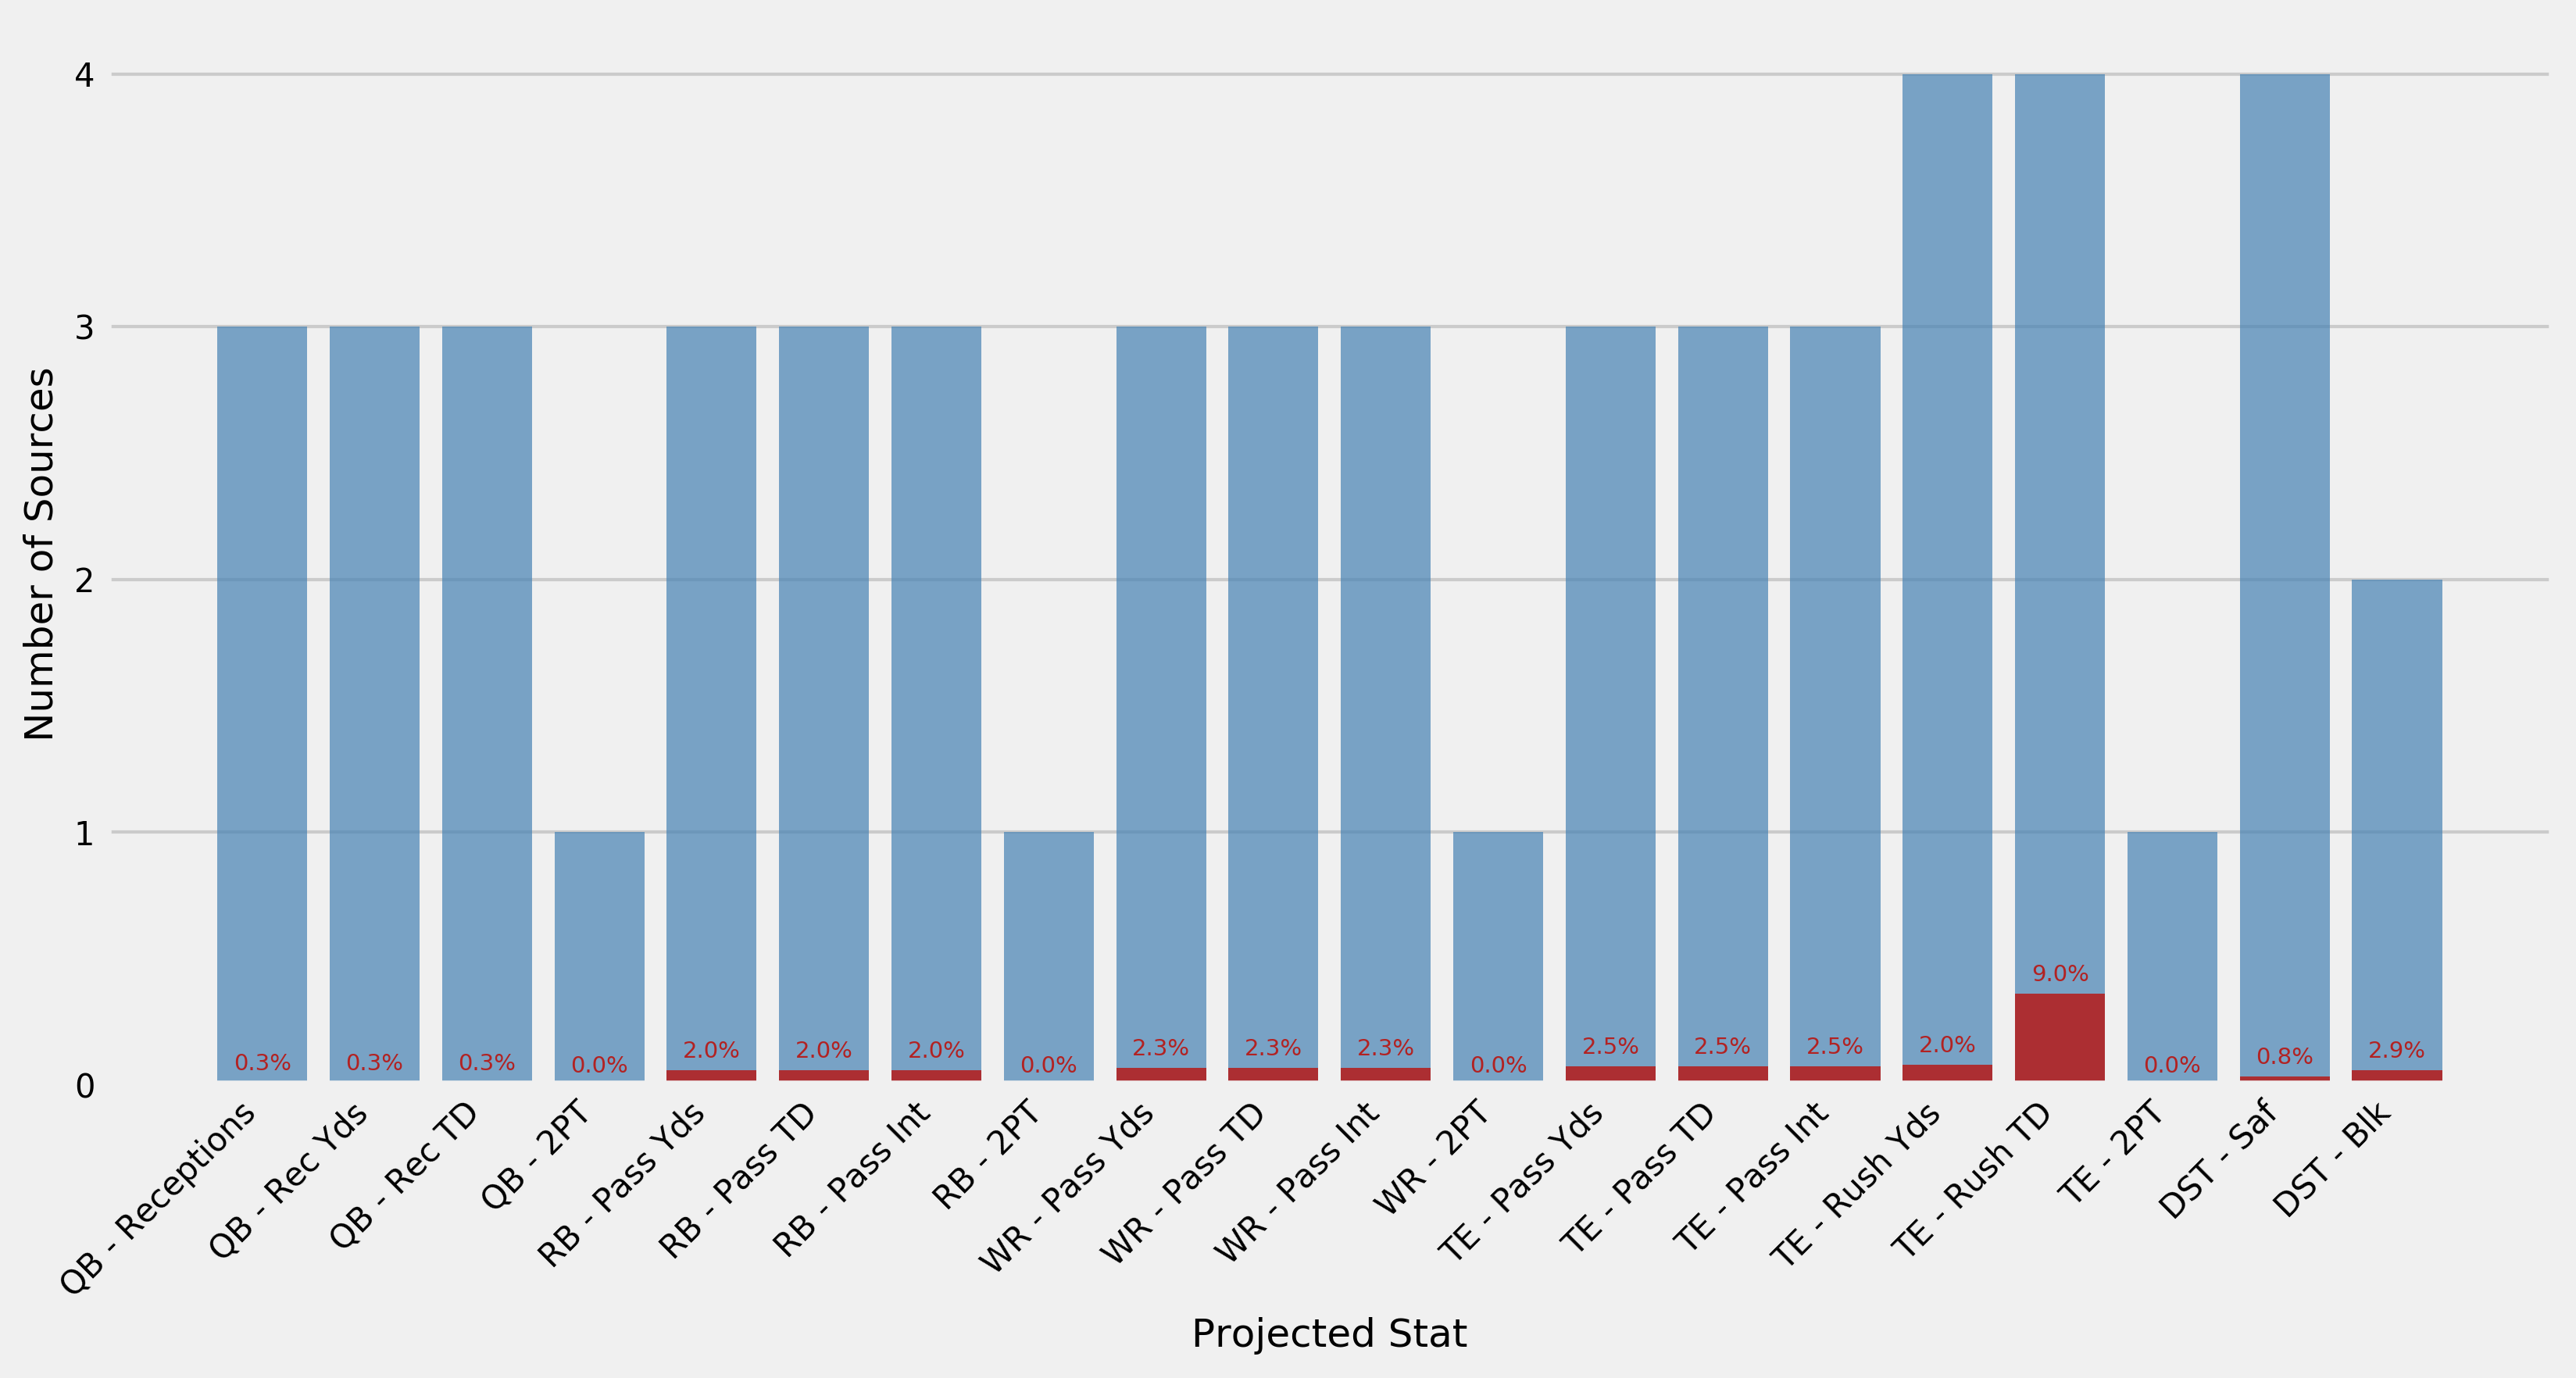
\includegraphics[width=0.95\textwidth]{../figures/nonessential_missing_data}
  \caption{Number of sources collected for each nonessential stat (blue). Red  indicates percentage of missing data for each respective stat.}
\end{figure}

\begin{figure}[H]
  \centering
  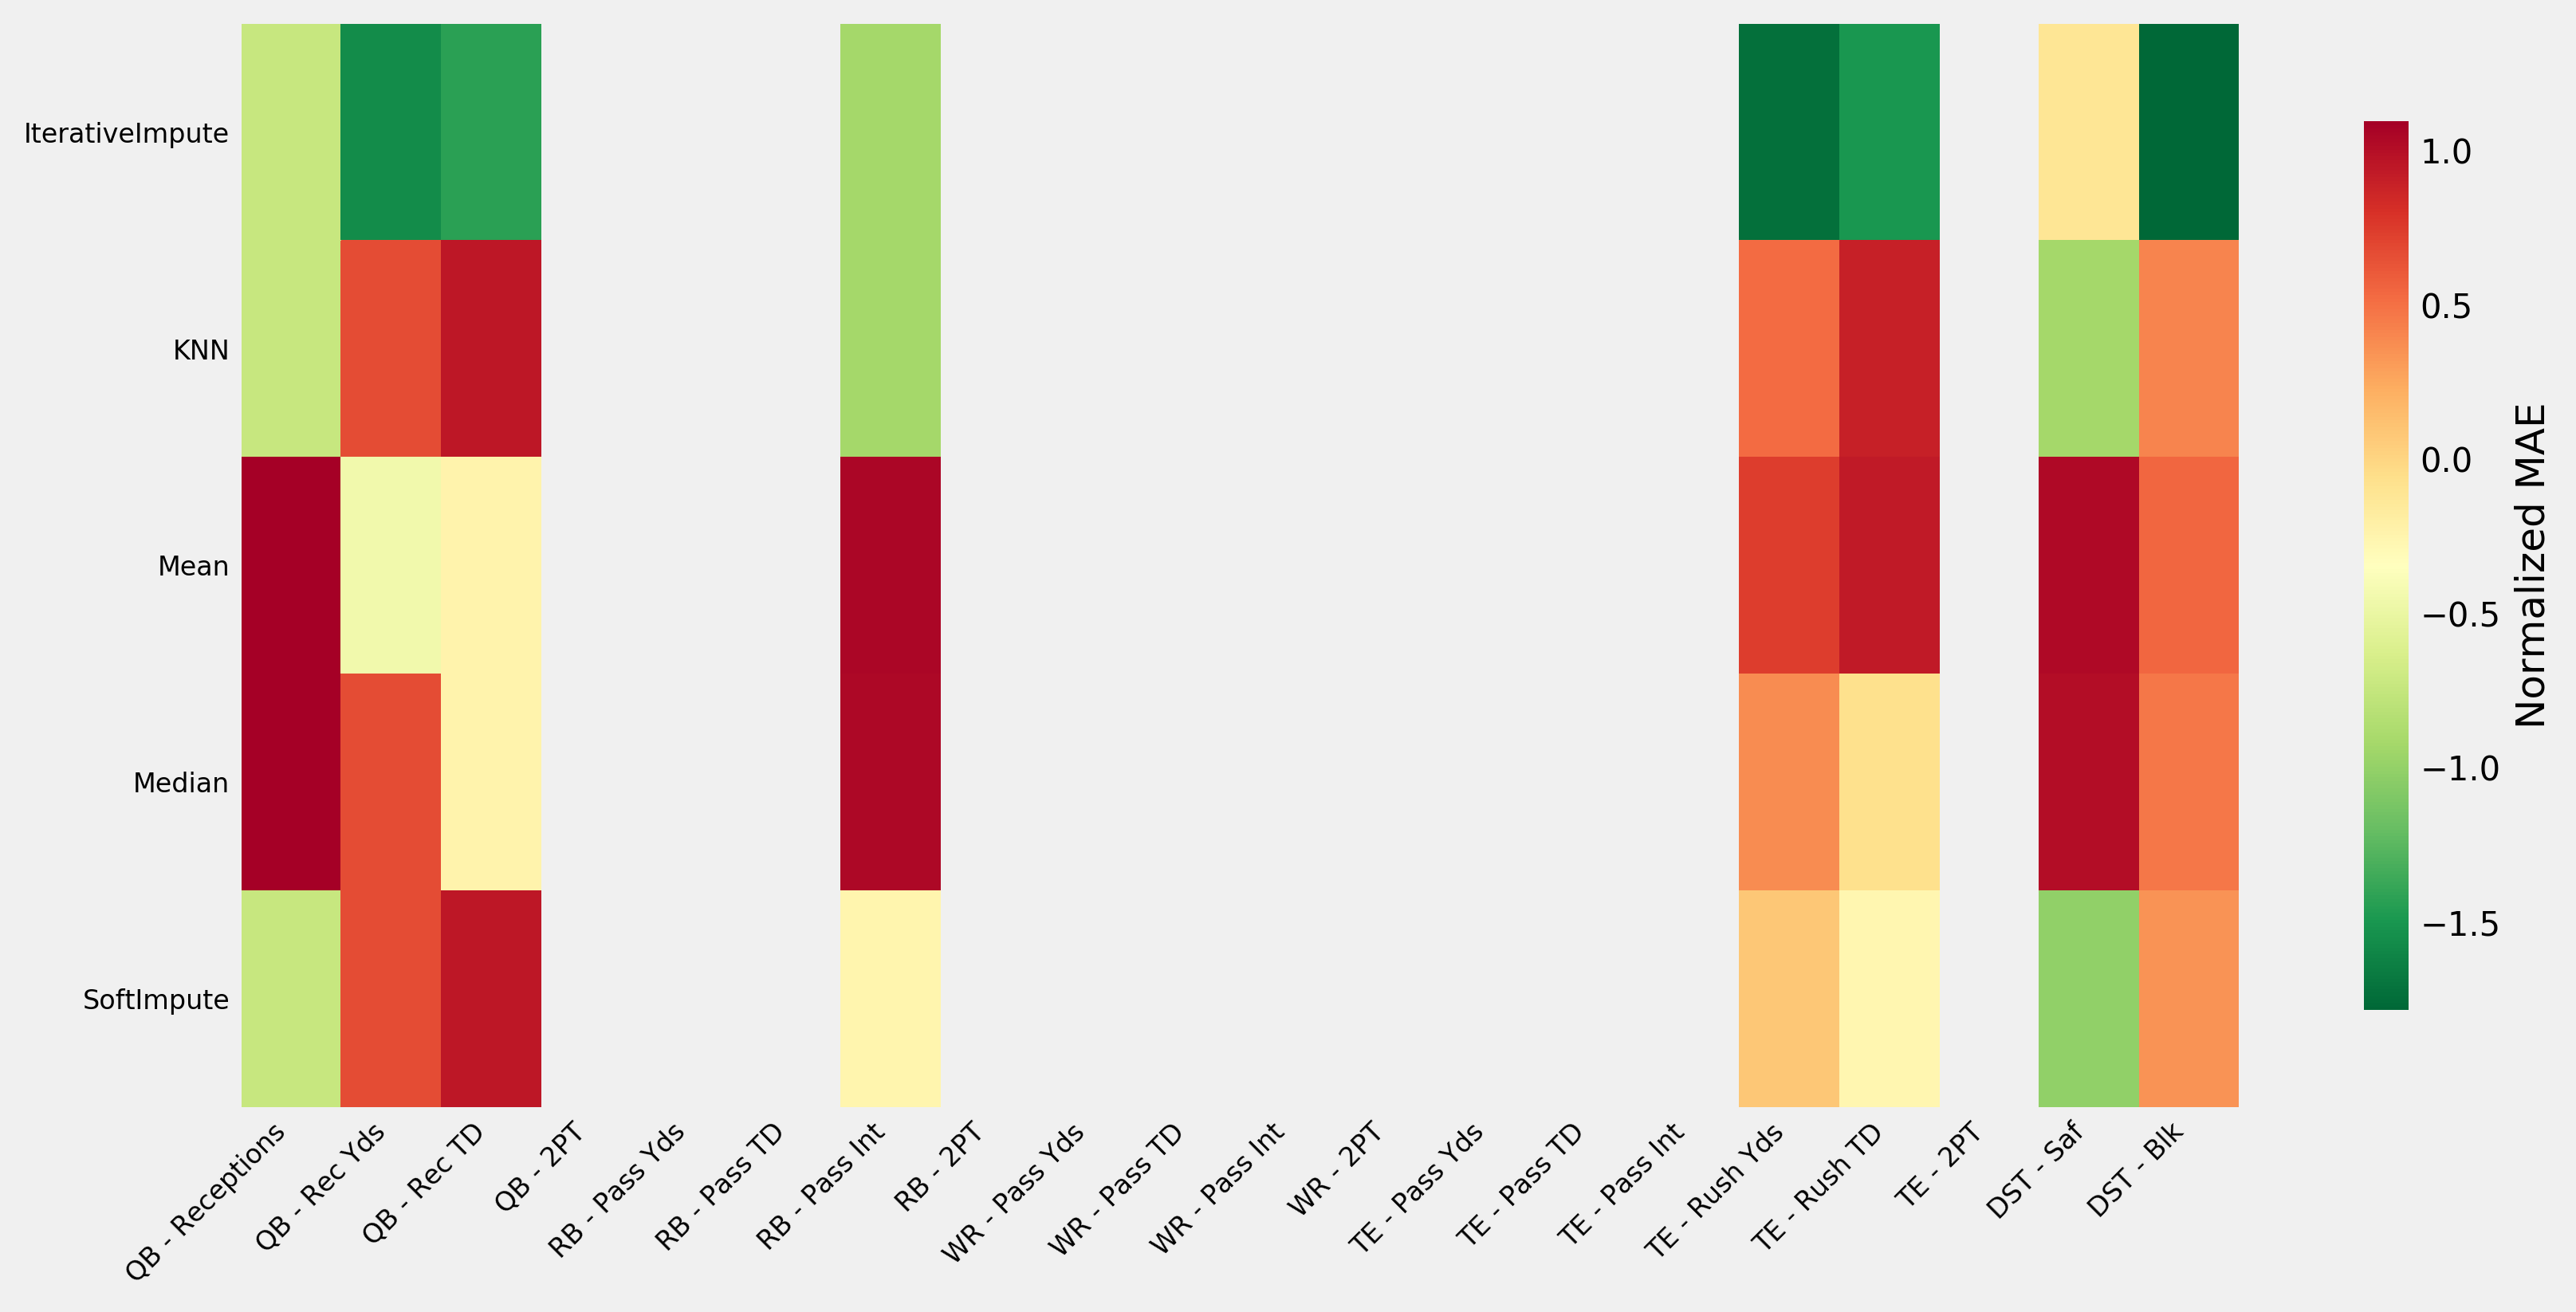
\includegraphics[width=0.95\textwidth]{../figures/nonessential_impute_MAE}
  \caption{Normalized MAE of imputing methods for each nonessential stat.}
\end{figure}

\begin{figure}[H]
  \centering
  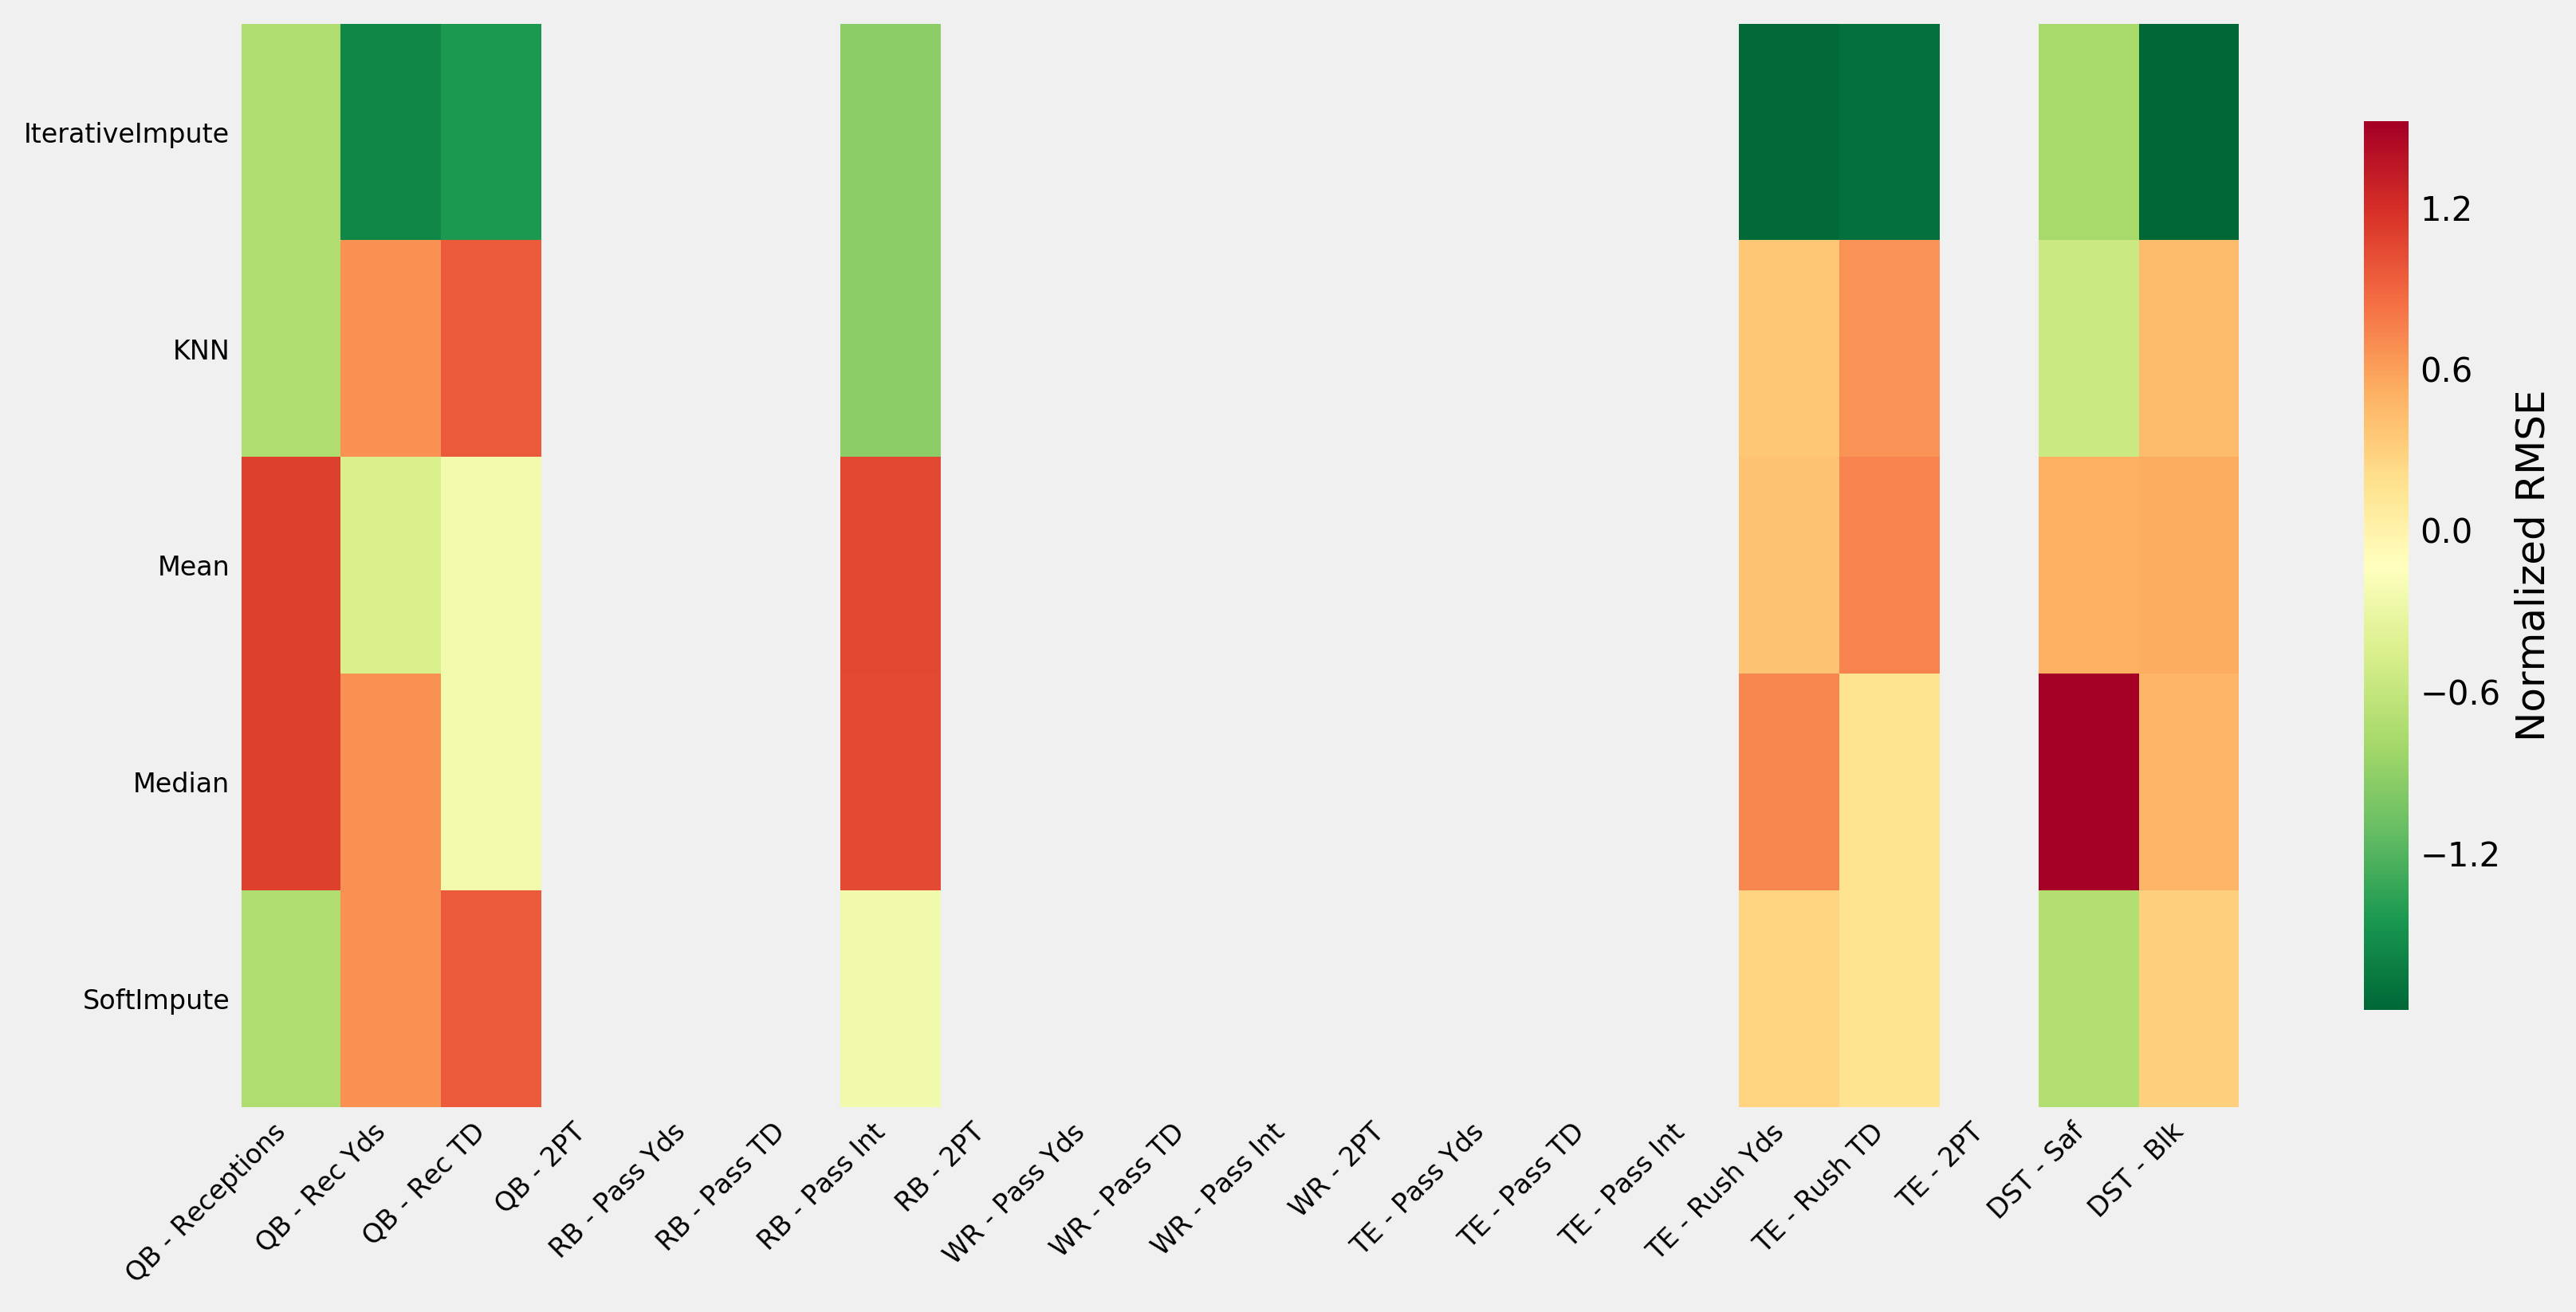
\includegraphics[width=0.95\textwidth]{../figures/nonessential_impute_RMSE}
  \caption{Normalized RMSE of imputing methods for each nonessential stat.}
\end{figure}

\pagebreak
\section{Essential Stats Histograms}

\begin{figure}[H]
  \centering
  \begin{subfigure}[b]{0.450\textwidth}
    \centering
    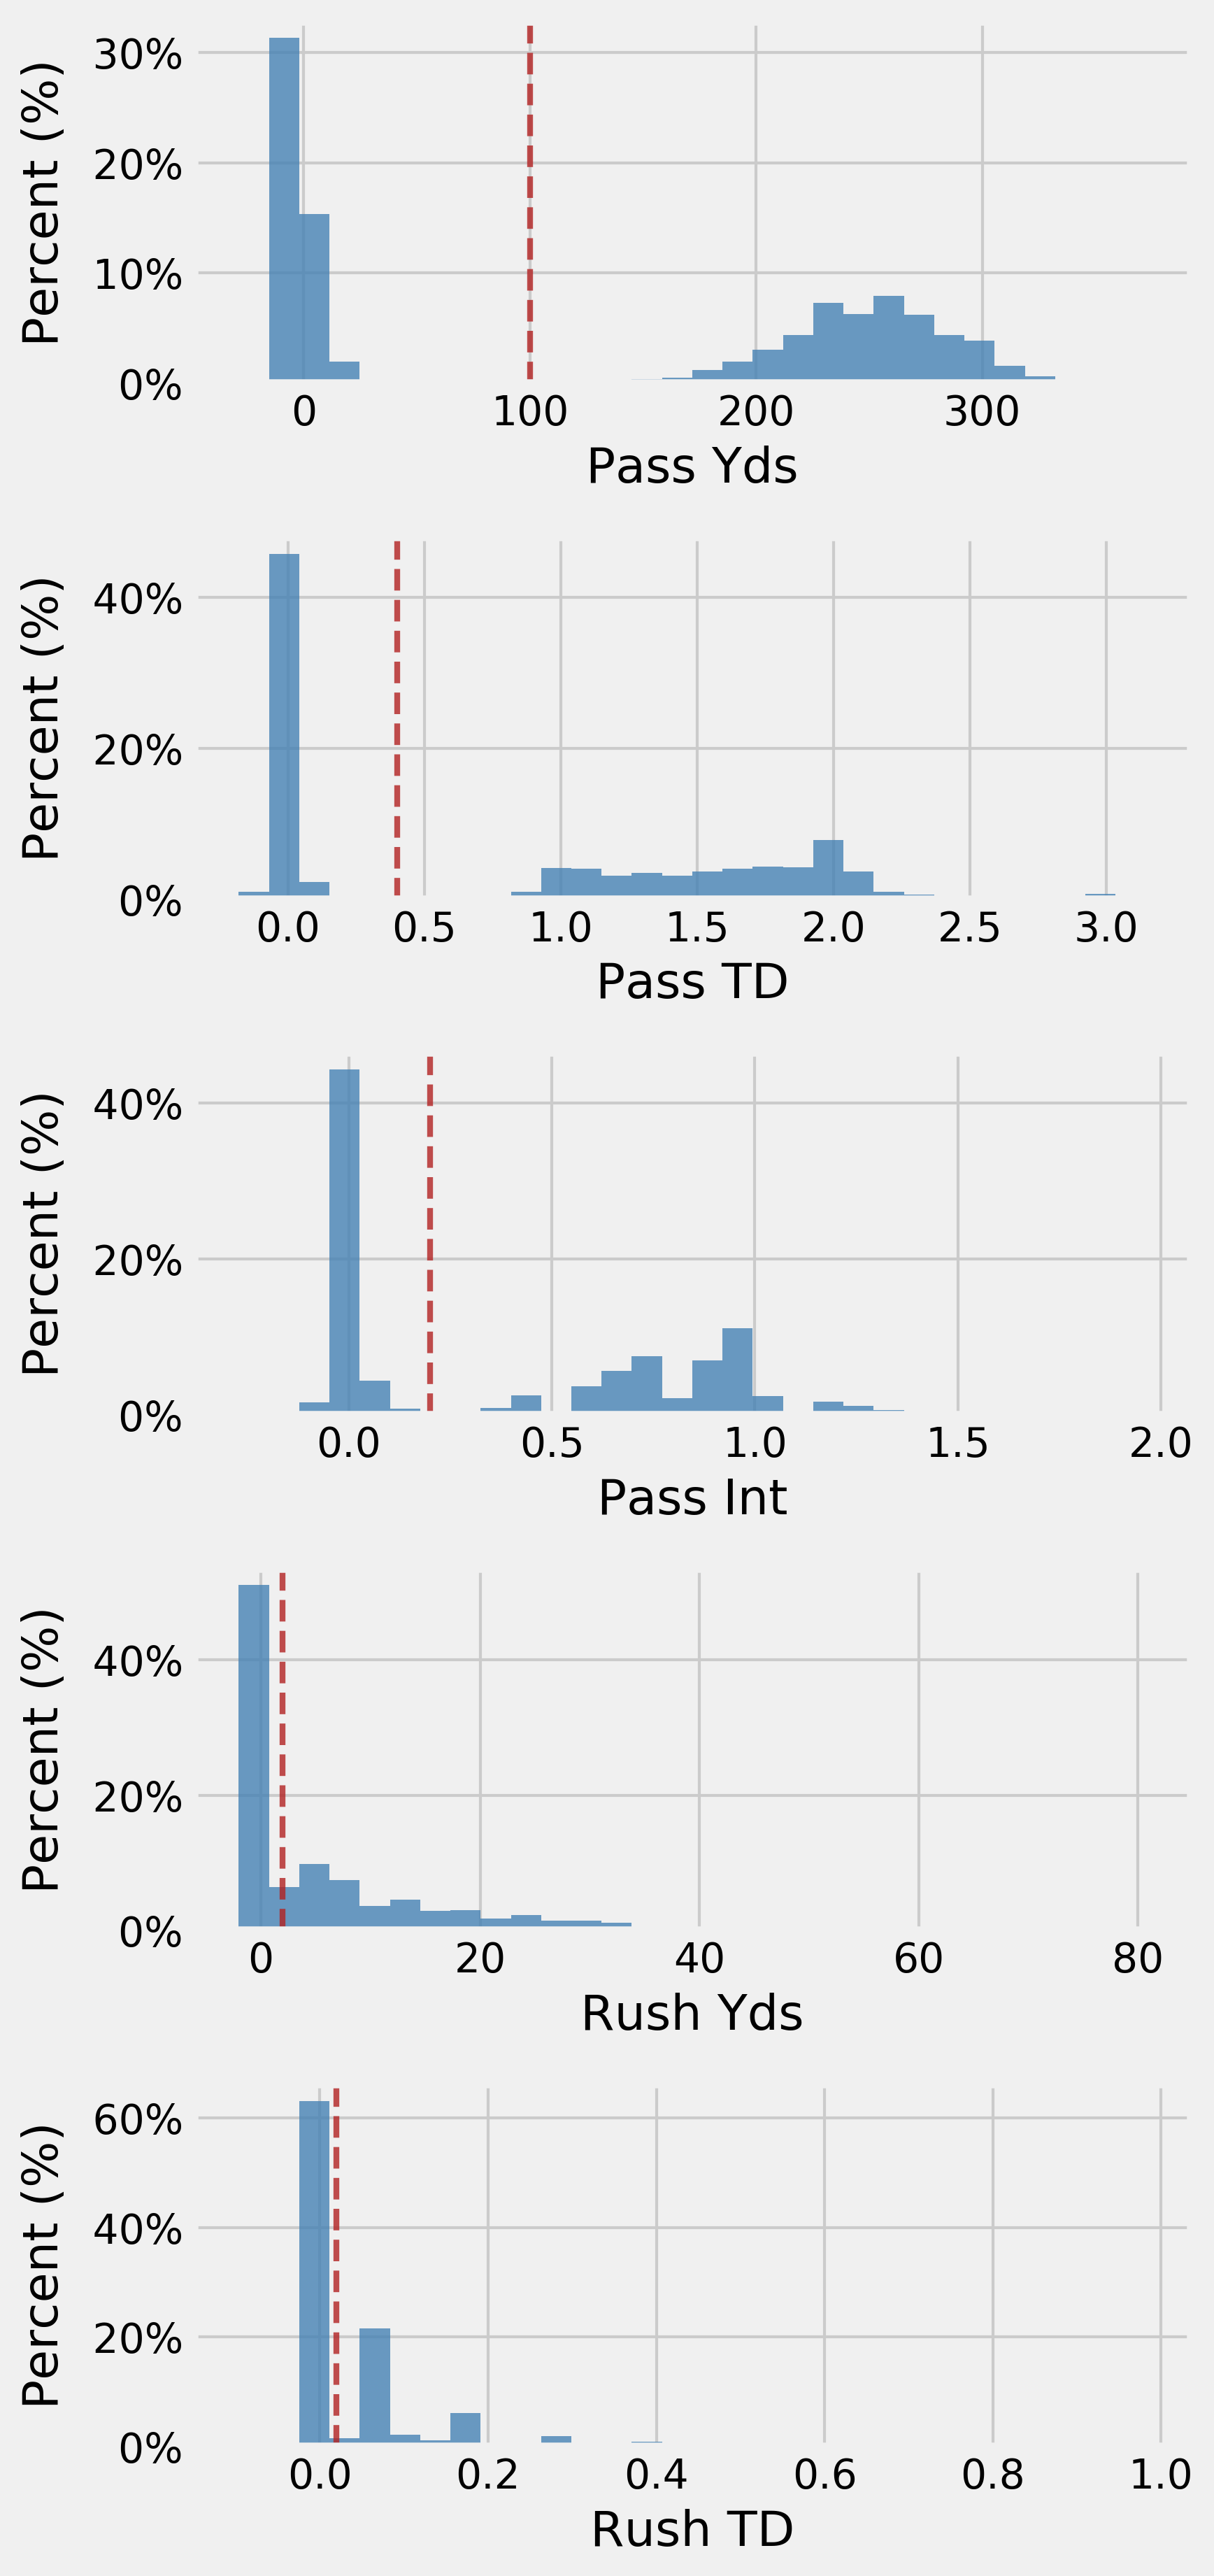
\includegraphics[width=1\textwidth]{../figures/no_threshold_hist_QB}
    \caption{Raw histogram with threshold (red).}
  \end{subfigure}
  \hfill
  \begin{subfigure}[b]{0.450\textwidth}
    \centering
    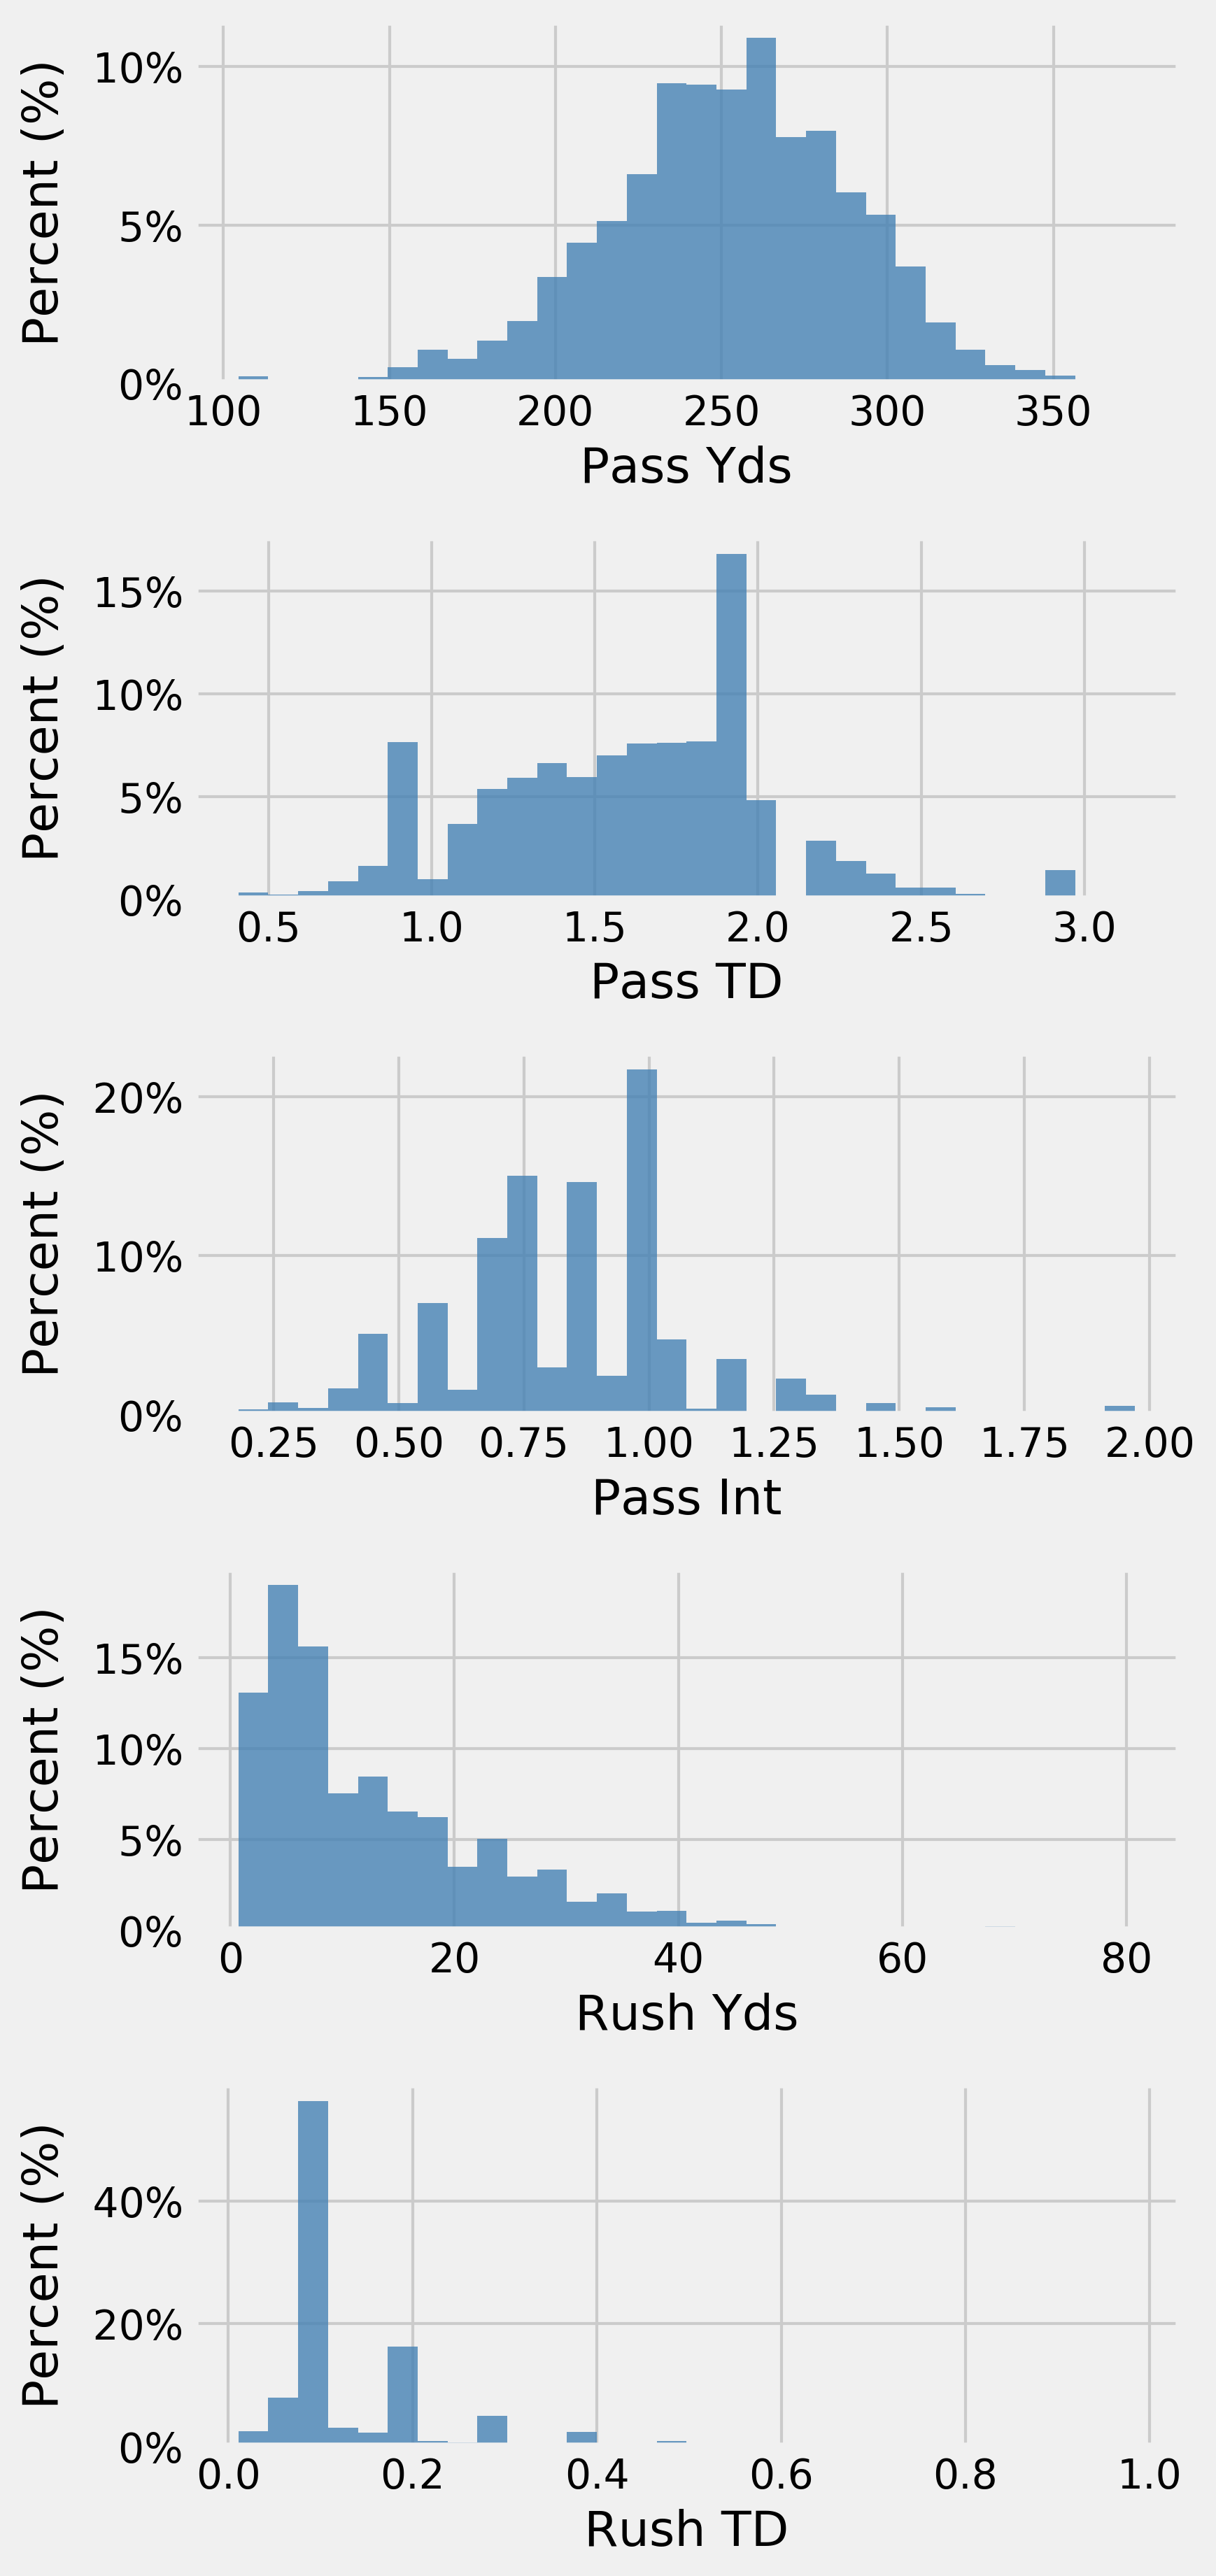
\includegraphics[width=1\textwidth]{../figures/threshold_hist_QB}
    \caption{Histogram above threshold.}
  \end{subfigure}
  \caption{Essential stat raw histograms and thresholded histograms for QB.}
\end{figure}

\pagebreak
\begin{figure}[H]
  \centering
  \begin{subfigure}[b]{0.450\textwidth}
    \centering
    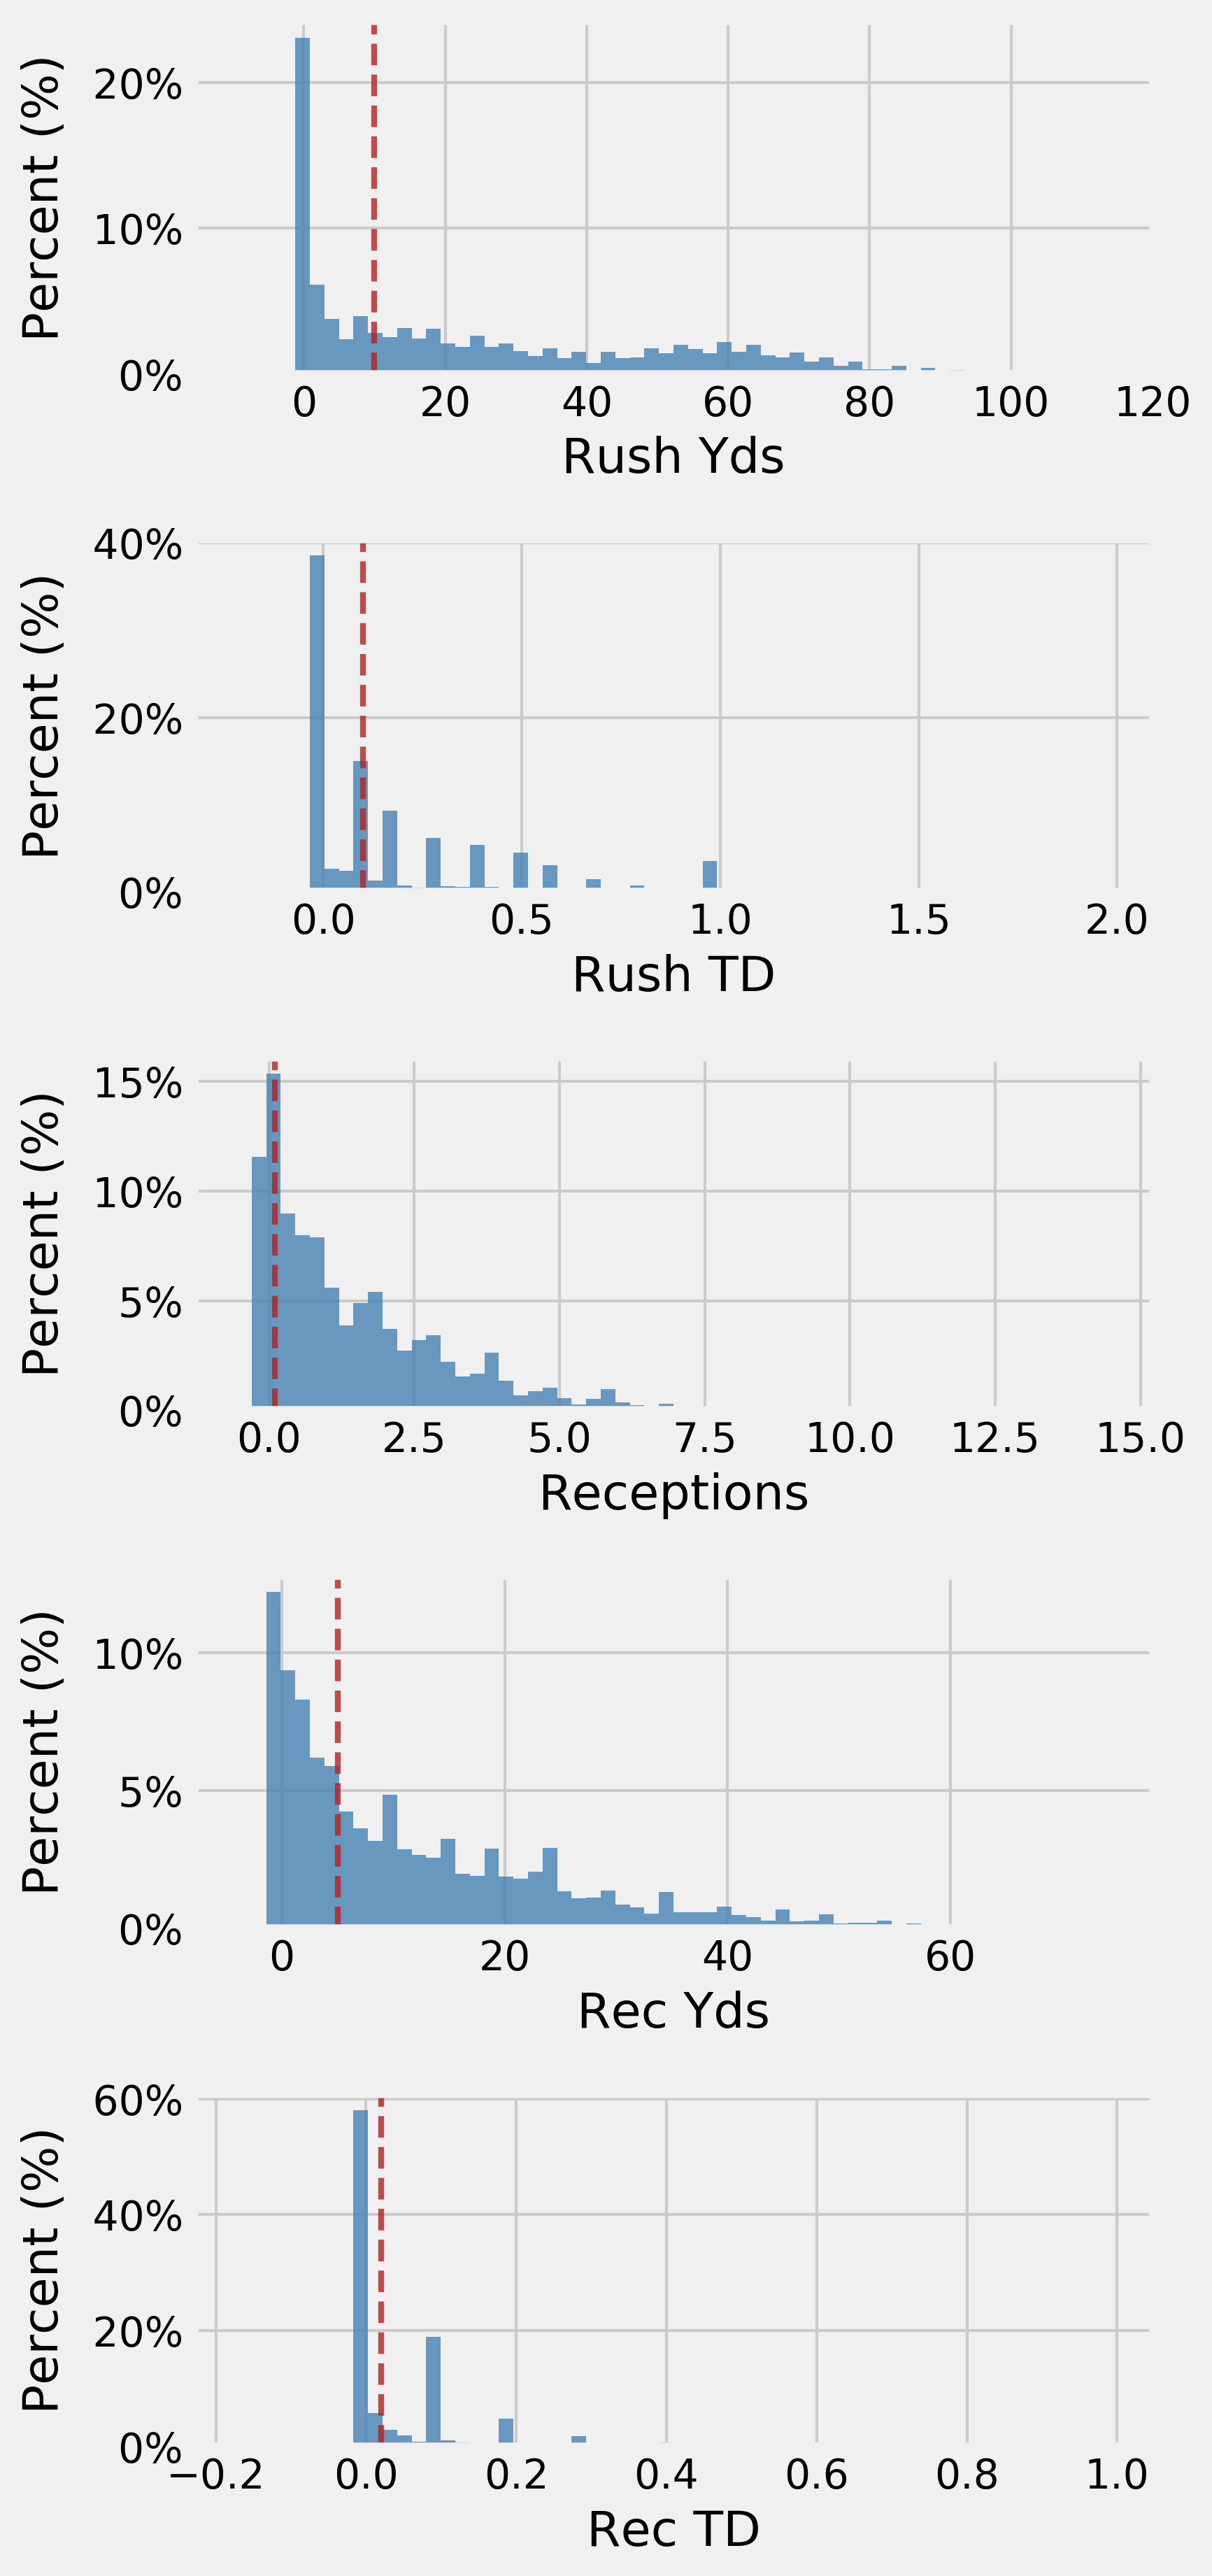
\includegraphics[width=1\textwidth]{../figures/no_threshold_hist_RB}
    \caption{Raw histogram with threshold (red).}
  \end{subfigure}
  \hfill
  \begin{subfigure}[b]{0.450\textwidth}
    \centering
    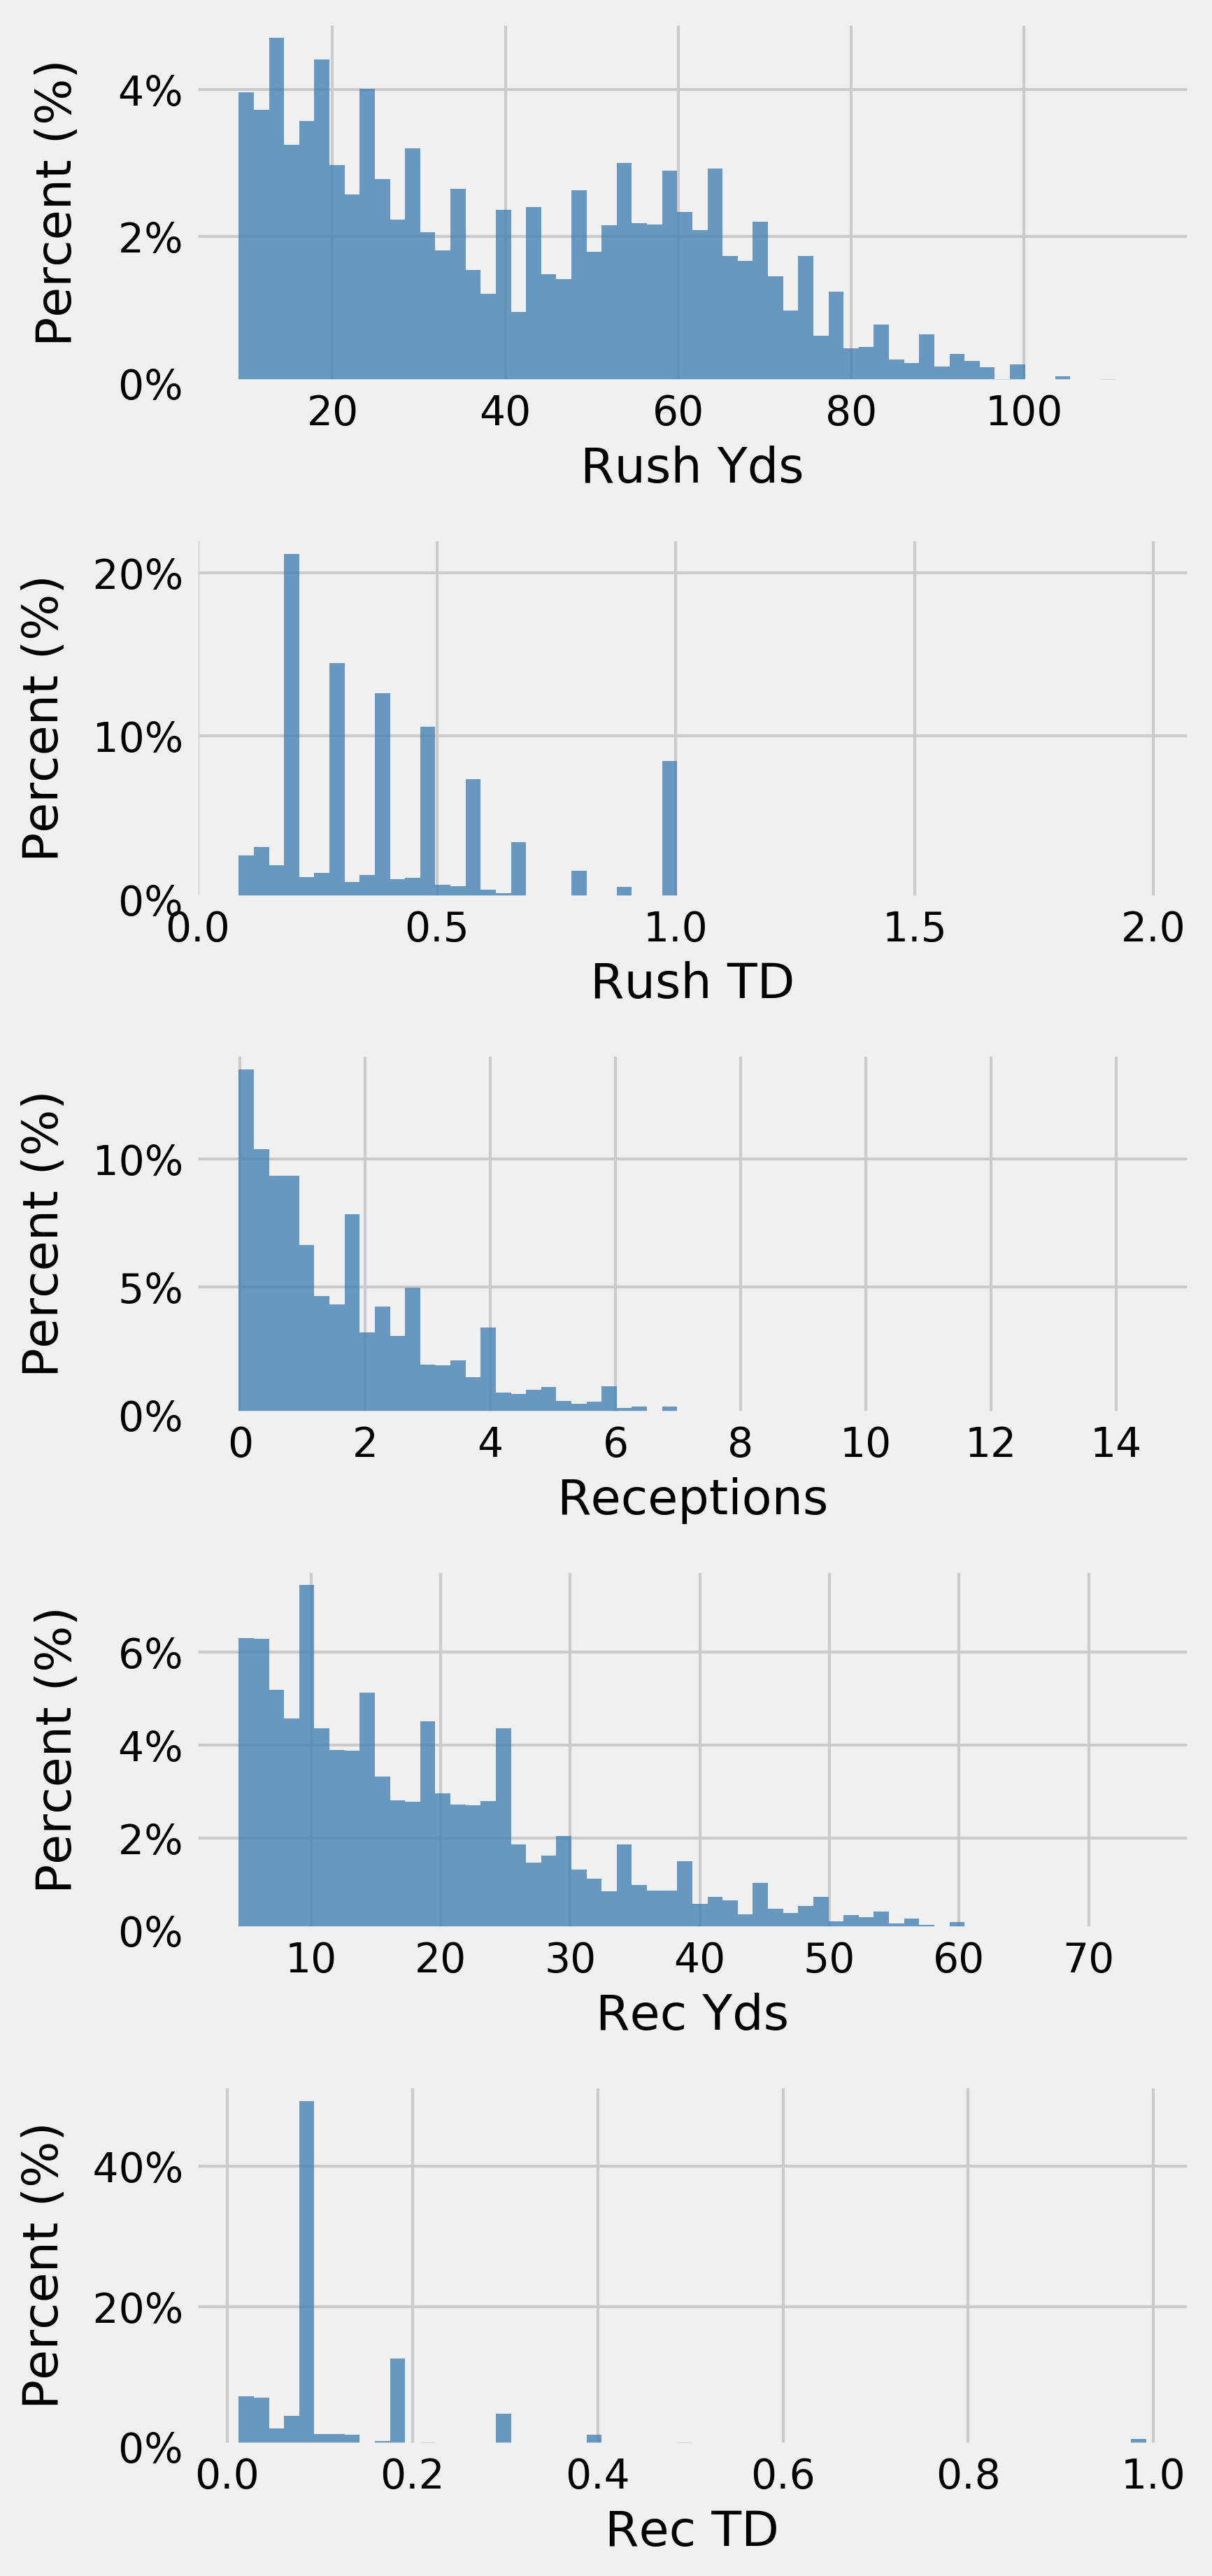
\includegraphics[width=1\textwidth]{../figures/threshold_hist_RB}
    \caption{Histogram above threshold.}
  \end{subfigure}
  \caption{Essential stat raw histograms and thresholded histograms for RB.}
\end{figure}

\pagebreak
\begin{figure}[H]
  \centering
  \begin{subfigure}[b]{0.450\textwidth}
    \centering
    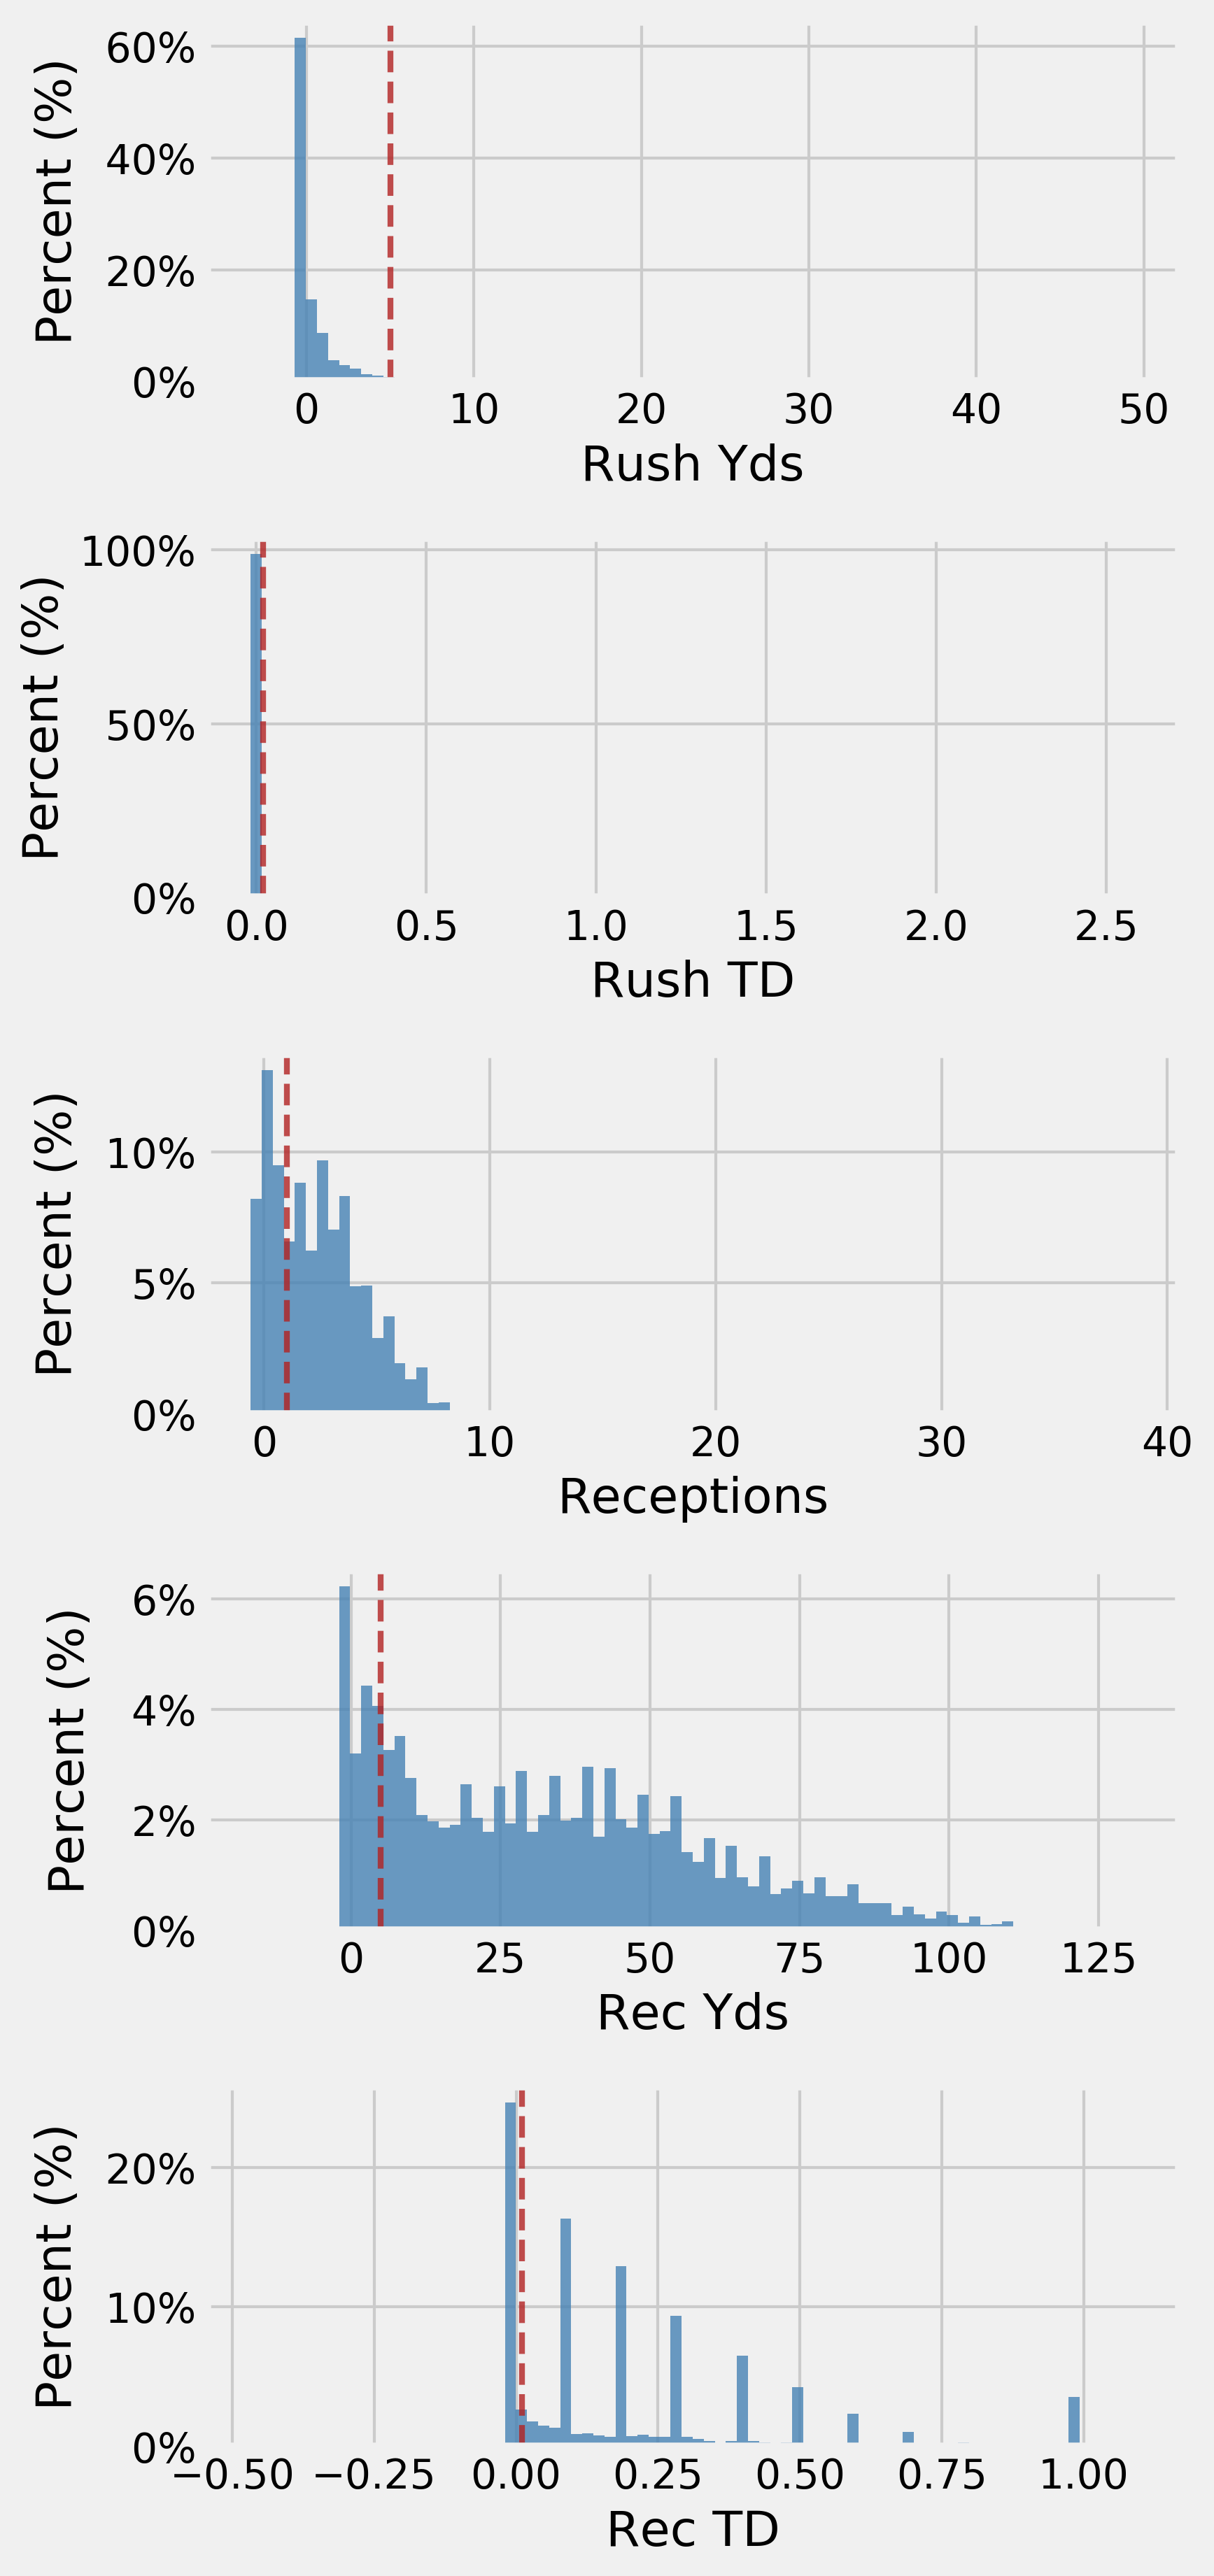
\includegraphics[width=1\textwidth]{../figures/no_threshold_hist_WR}
    \caption{Raw histogram with threshold (red).}
  \end{subfigure}
  \hfill
  \begin{subfigure}[b]{0.450\textwidth}
    \centering
    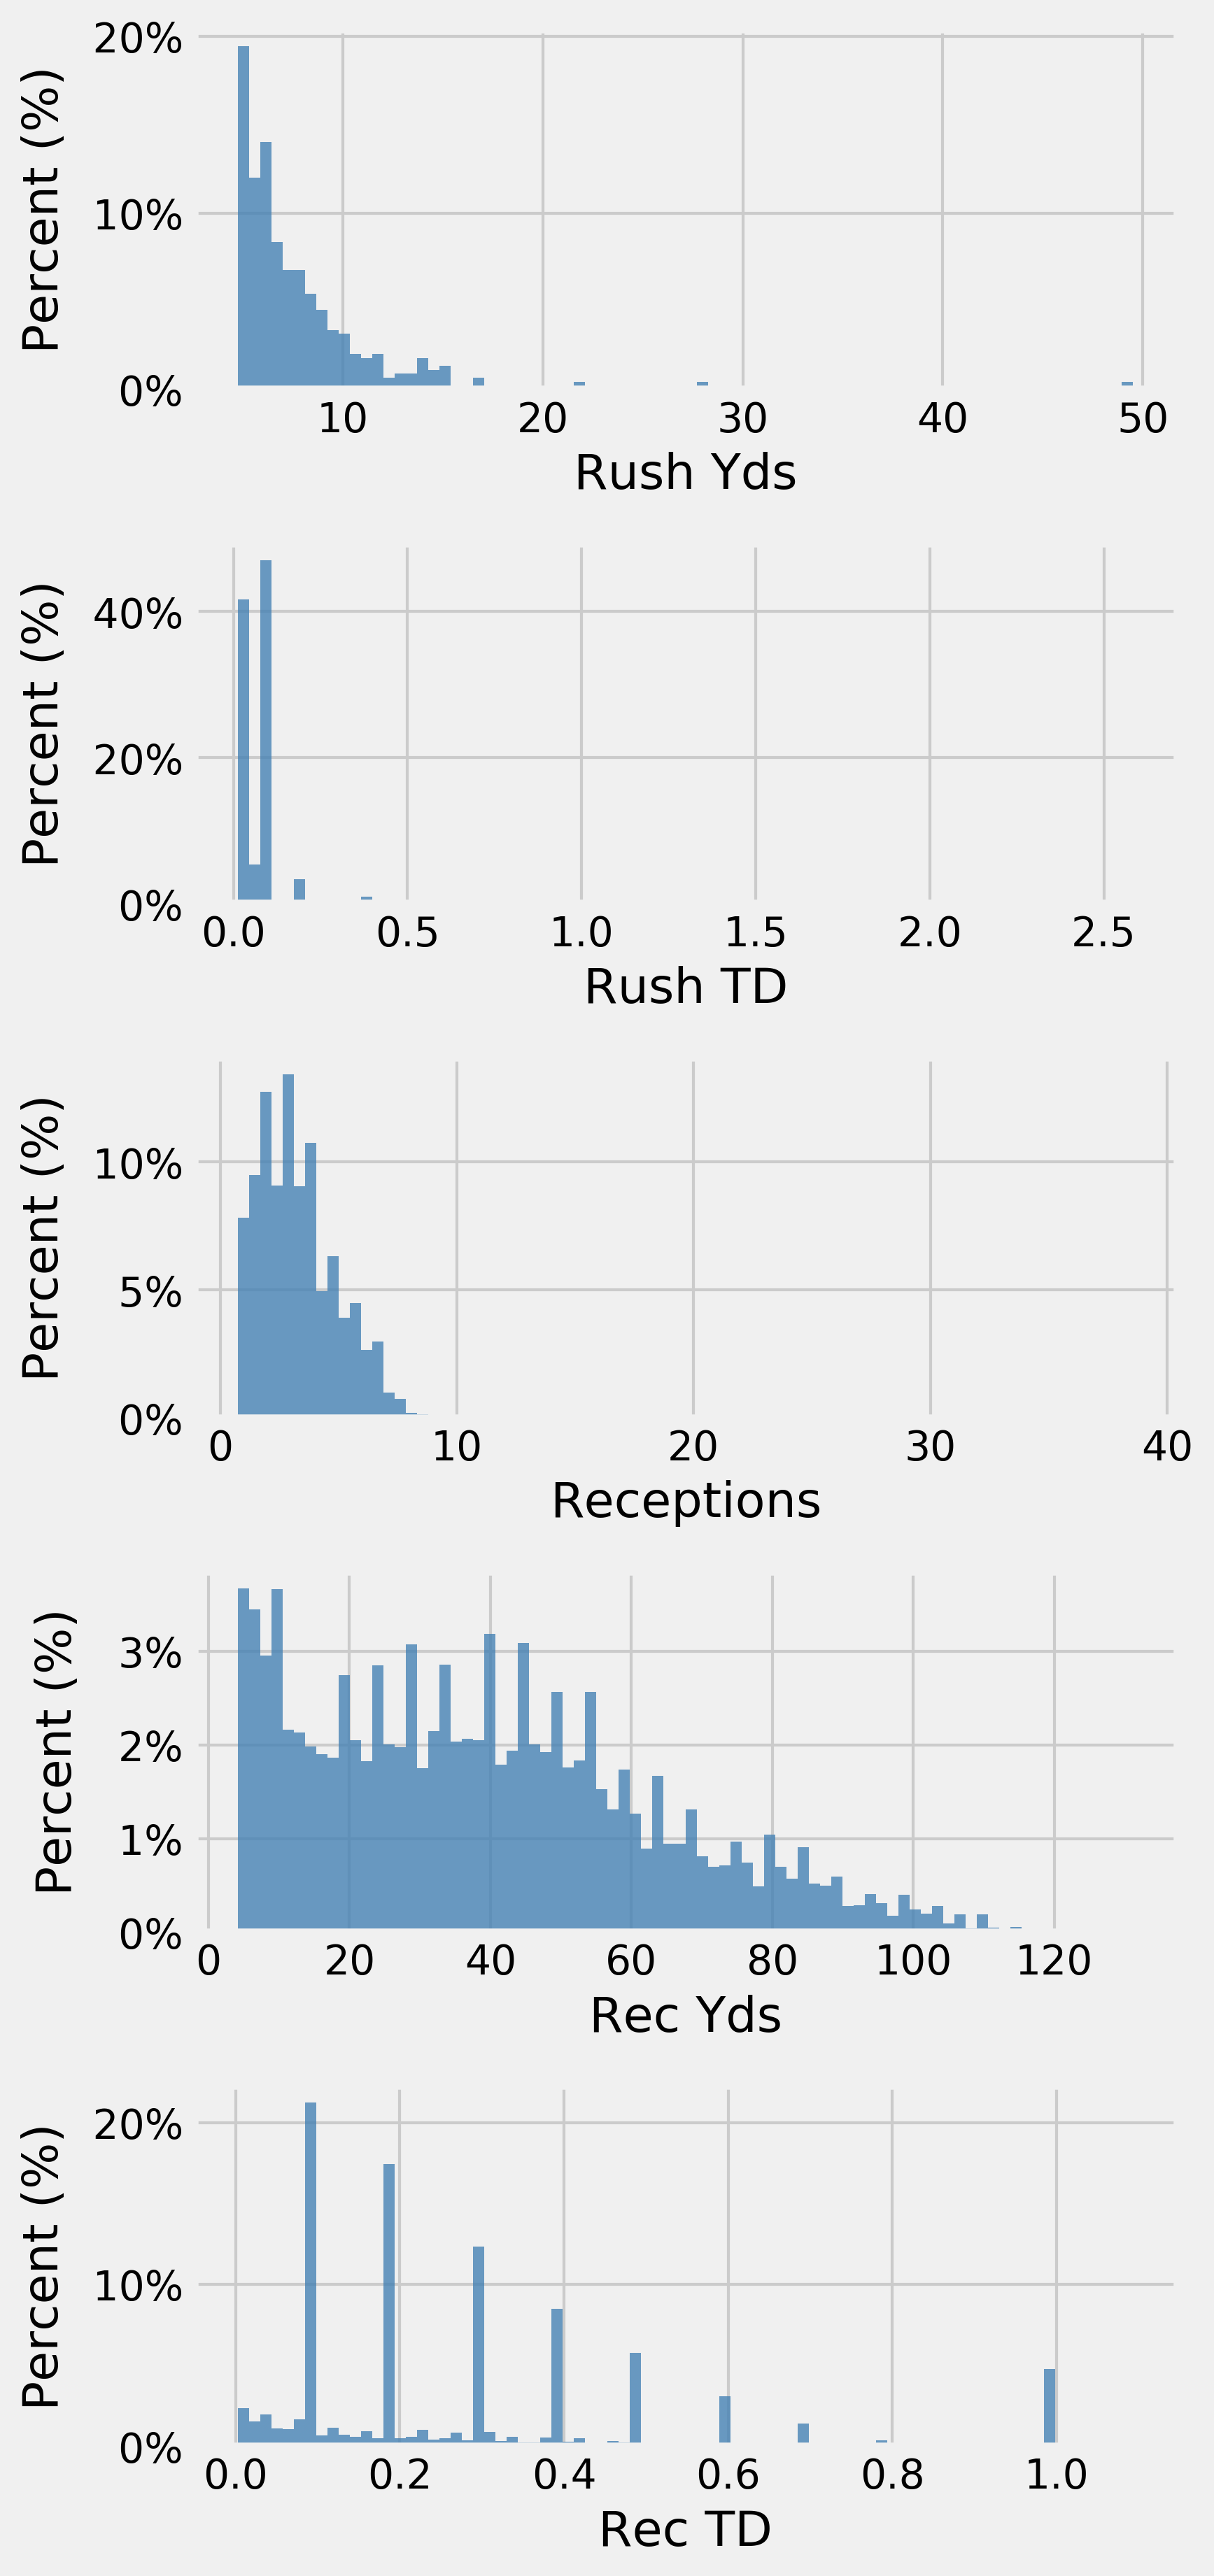
\includegraphics[width=1\textwidth]{../figures/threshold_hist_WR}
    \caption{Histogram above threshold.}
  \end{subfigure}
  \caption{Essential stat raw histograms and thresholded histograms for WR.}
\end{figure}

\pagebreak
\begin{figure}[H]
  \centering
  \begin{subfigure}[b]{0.450\textwidth}
    \centering
    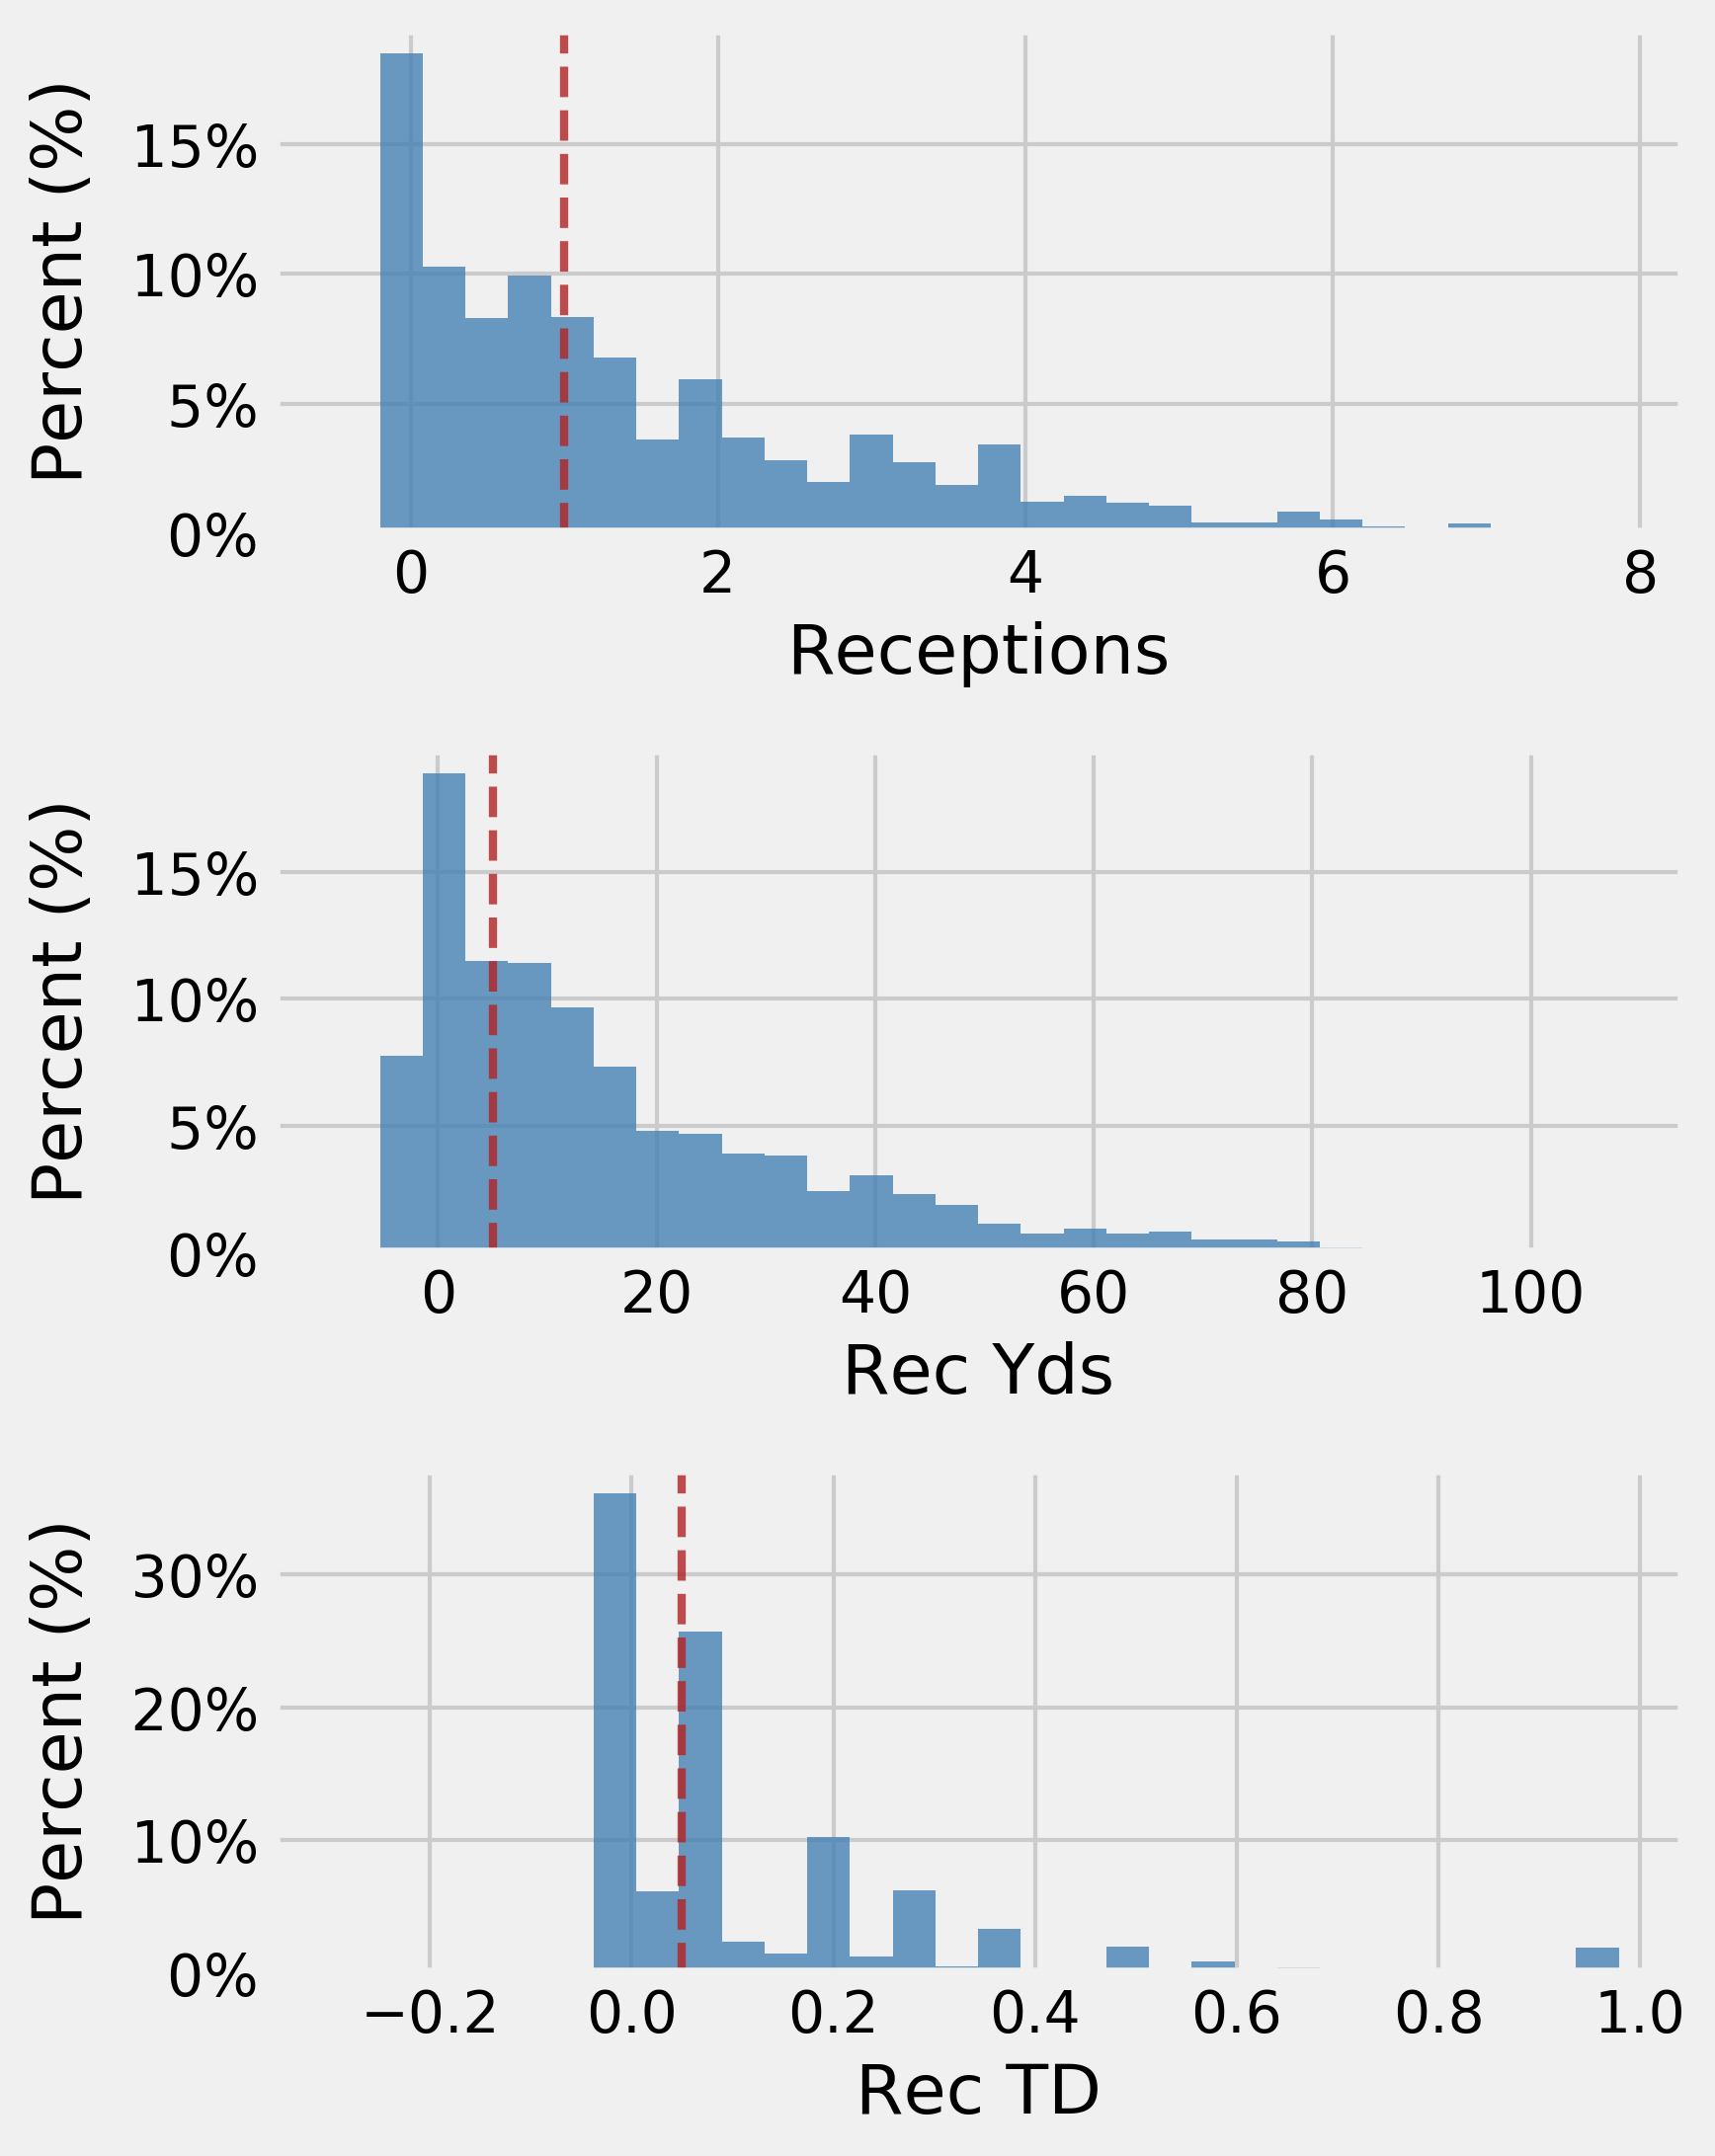
\includegraphics[width=1\textwidth]{../figures/no_threshold_hist_TE}
    \caption{Raw histogram with threshold (red).}
  \end{subfigure}
  \hfill
  \begin{subfigure}[b]{0.450\textwidth}
    \centering
    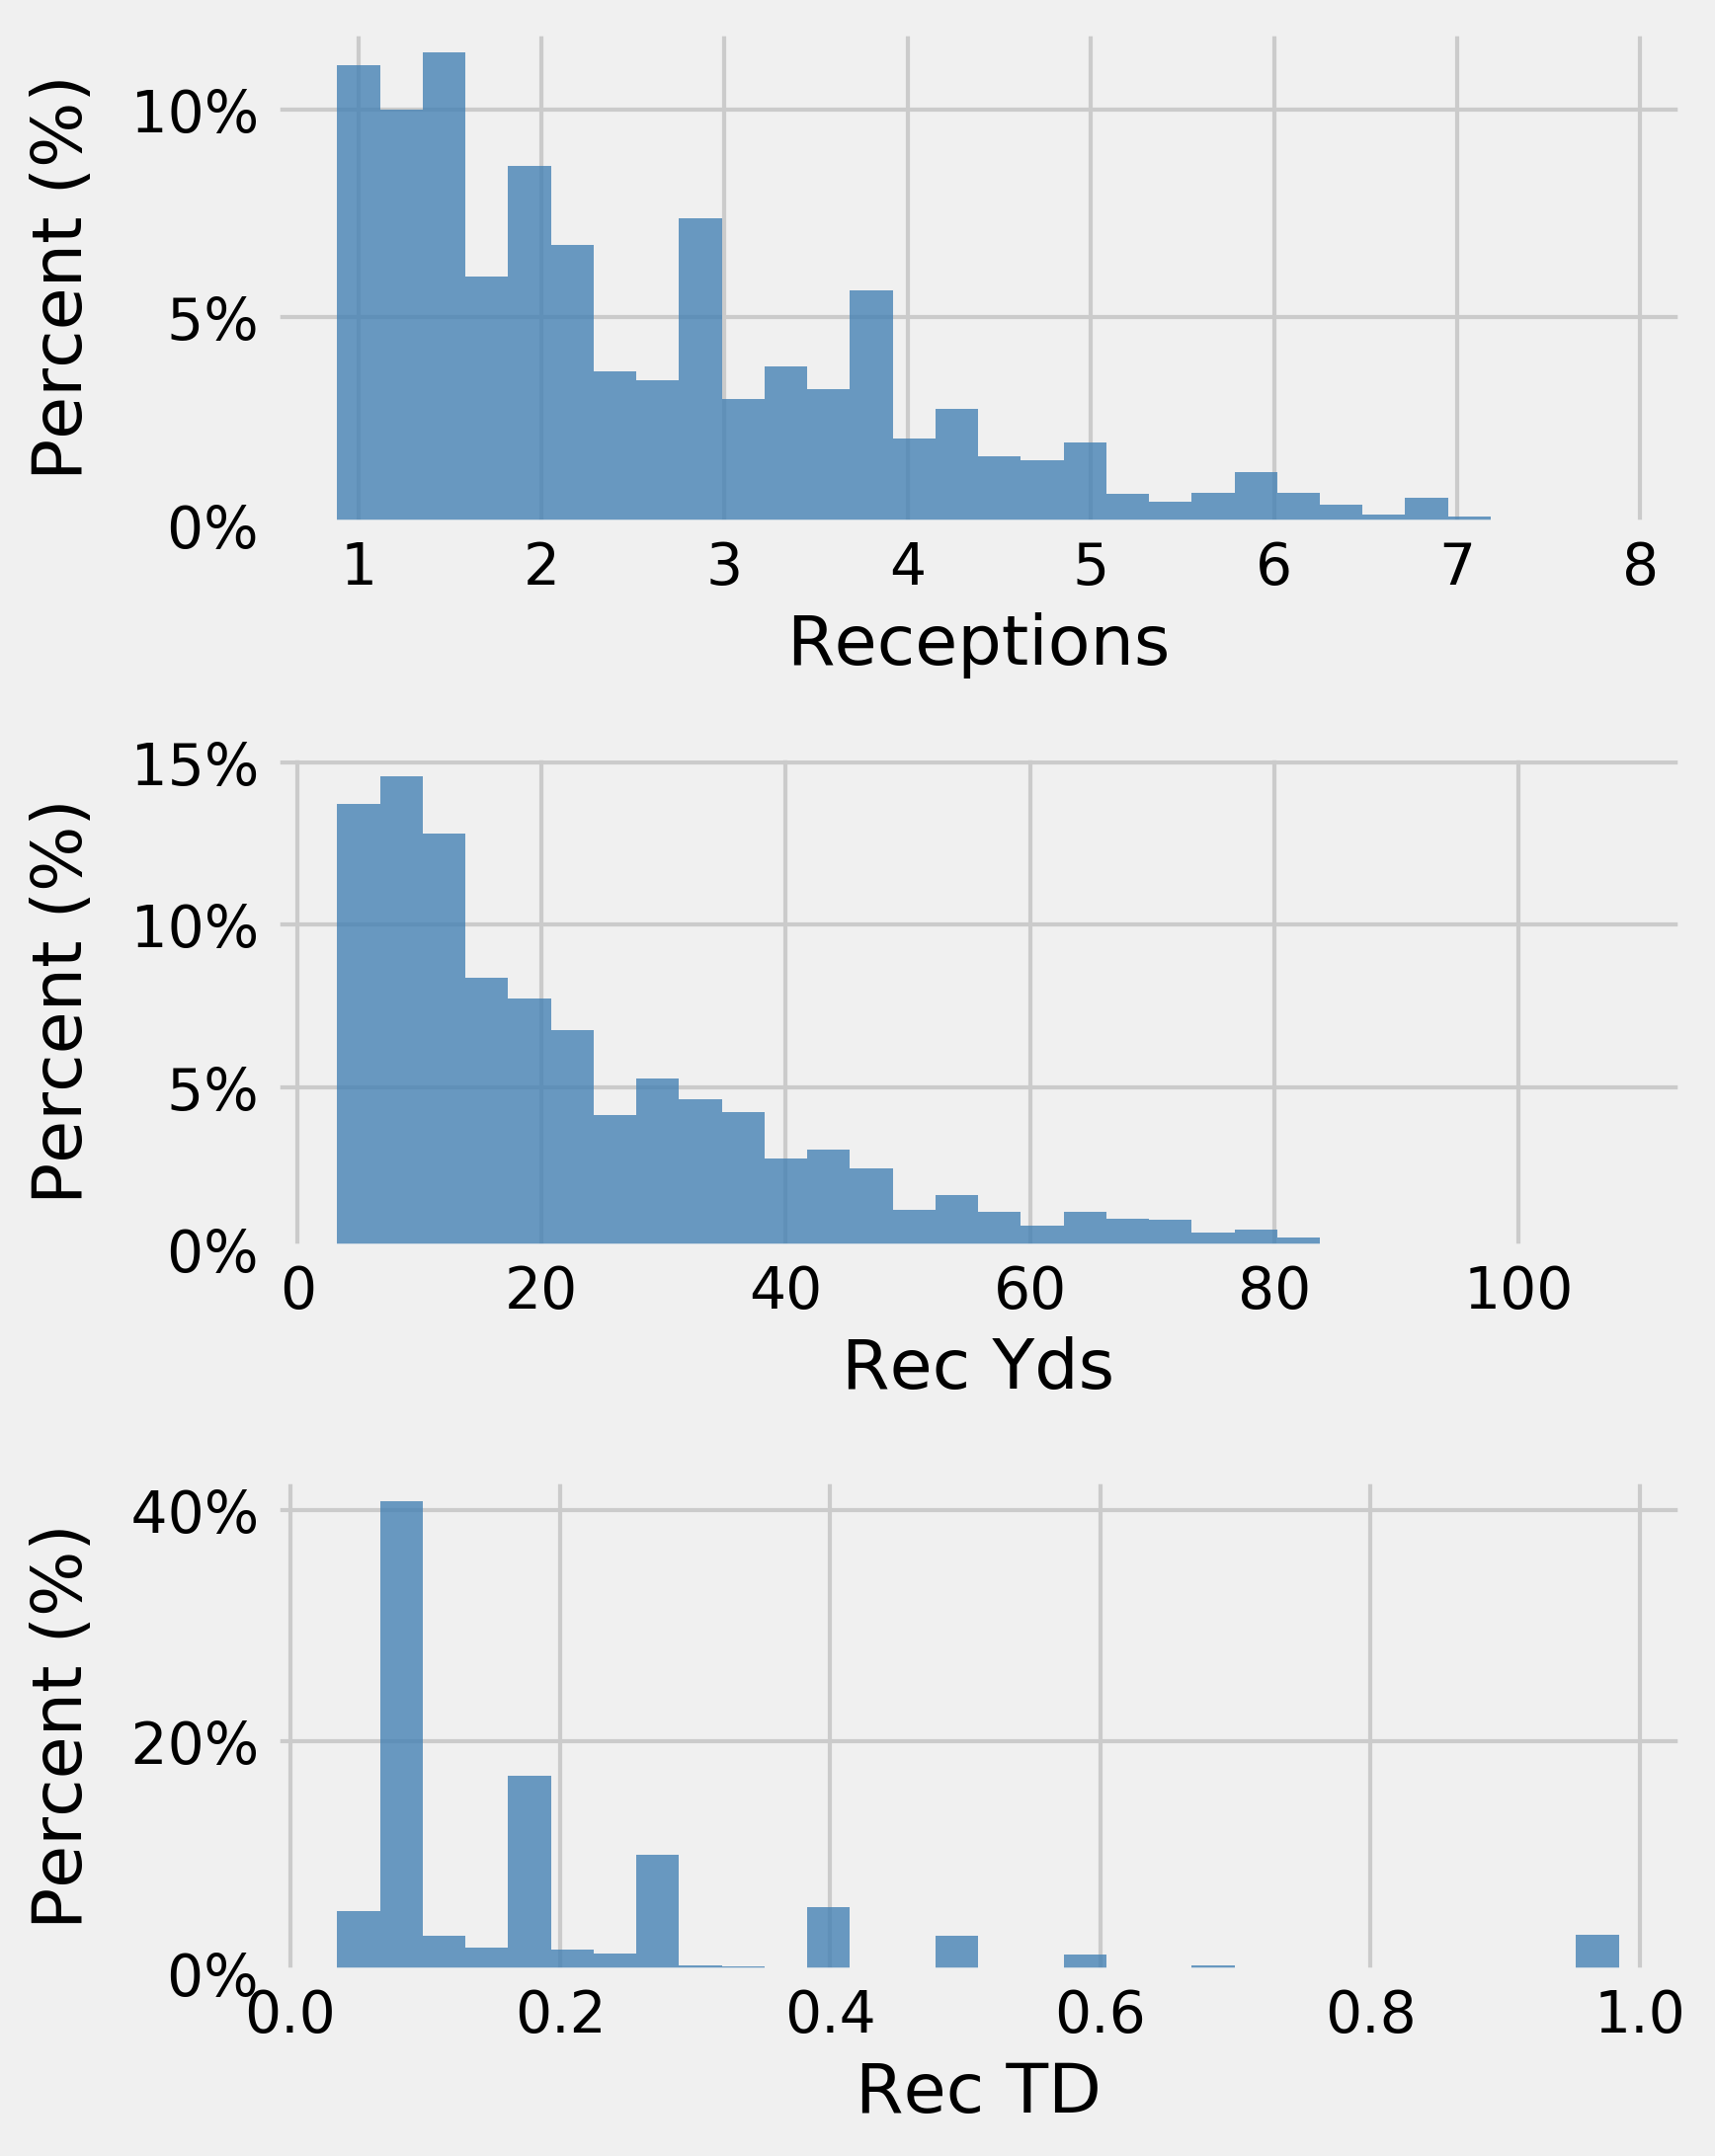
\includegraphics[width=1\textwidth]{../figures/threshold_hist_TE}
    \caption{Histogram above threshold.}
  \end{subfigure}
  \caption{Essential stat raw histograms and thresholded histograms for TE.}
\end{figure}

\pagebreak
\begin{figure}[H]
  \centering
  \begin{subfigure}[b]{0.450\textwidth}
    \centering
    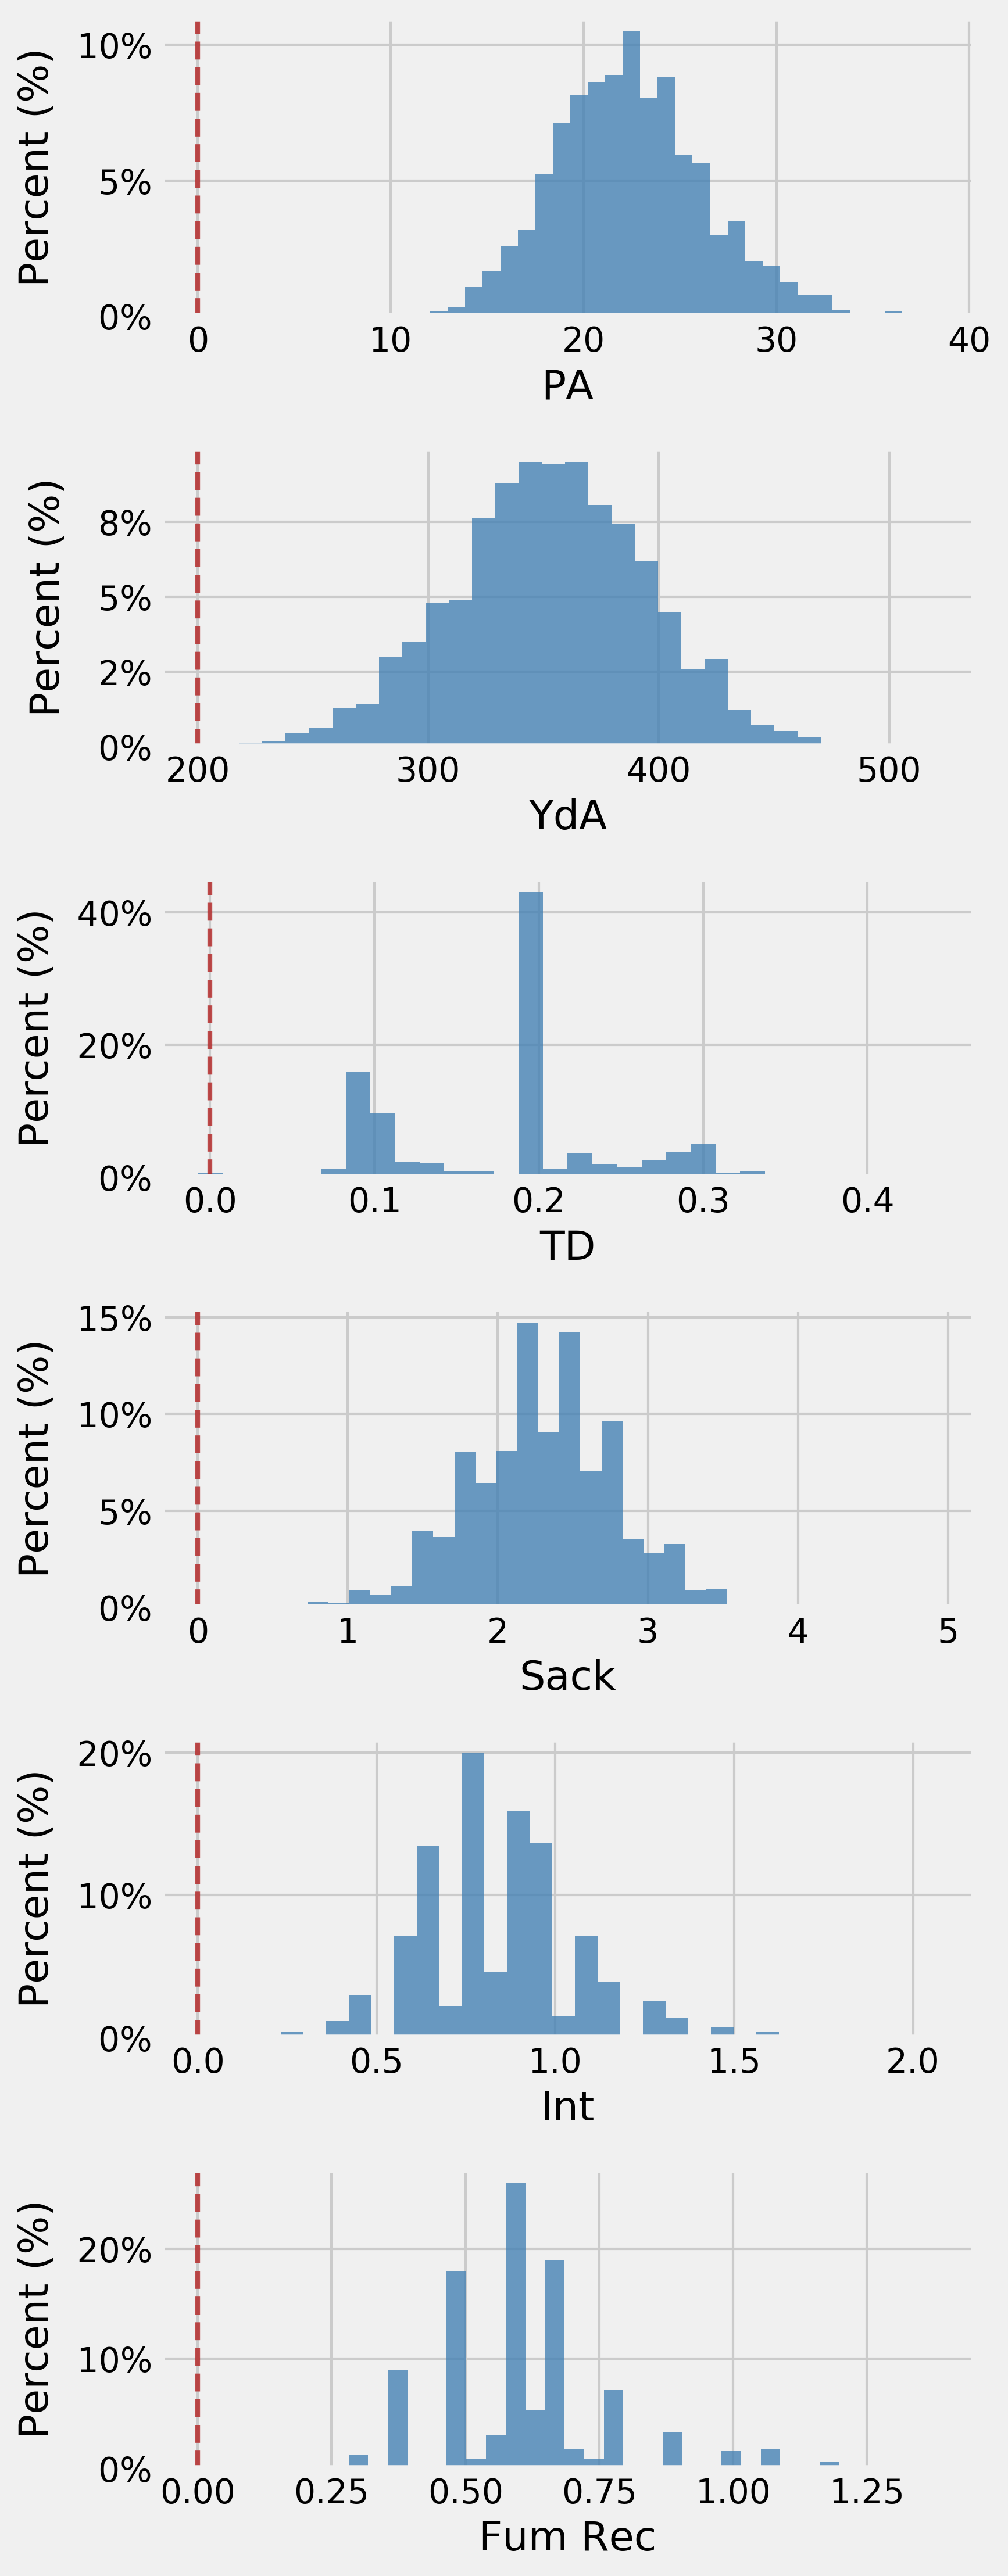
\includegraphics[width=1\textwidth]{../figures/no_threshold_hist_DST}
    \caption{Raw histogram with threshold (red).}
  \end{subfigure}
  \hfill
  \begin{subfigure}[b]{0.450\textwidth}
    \centering
    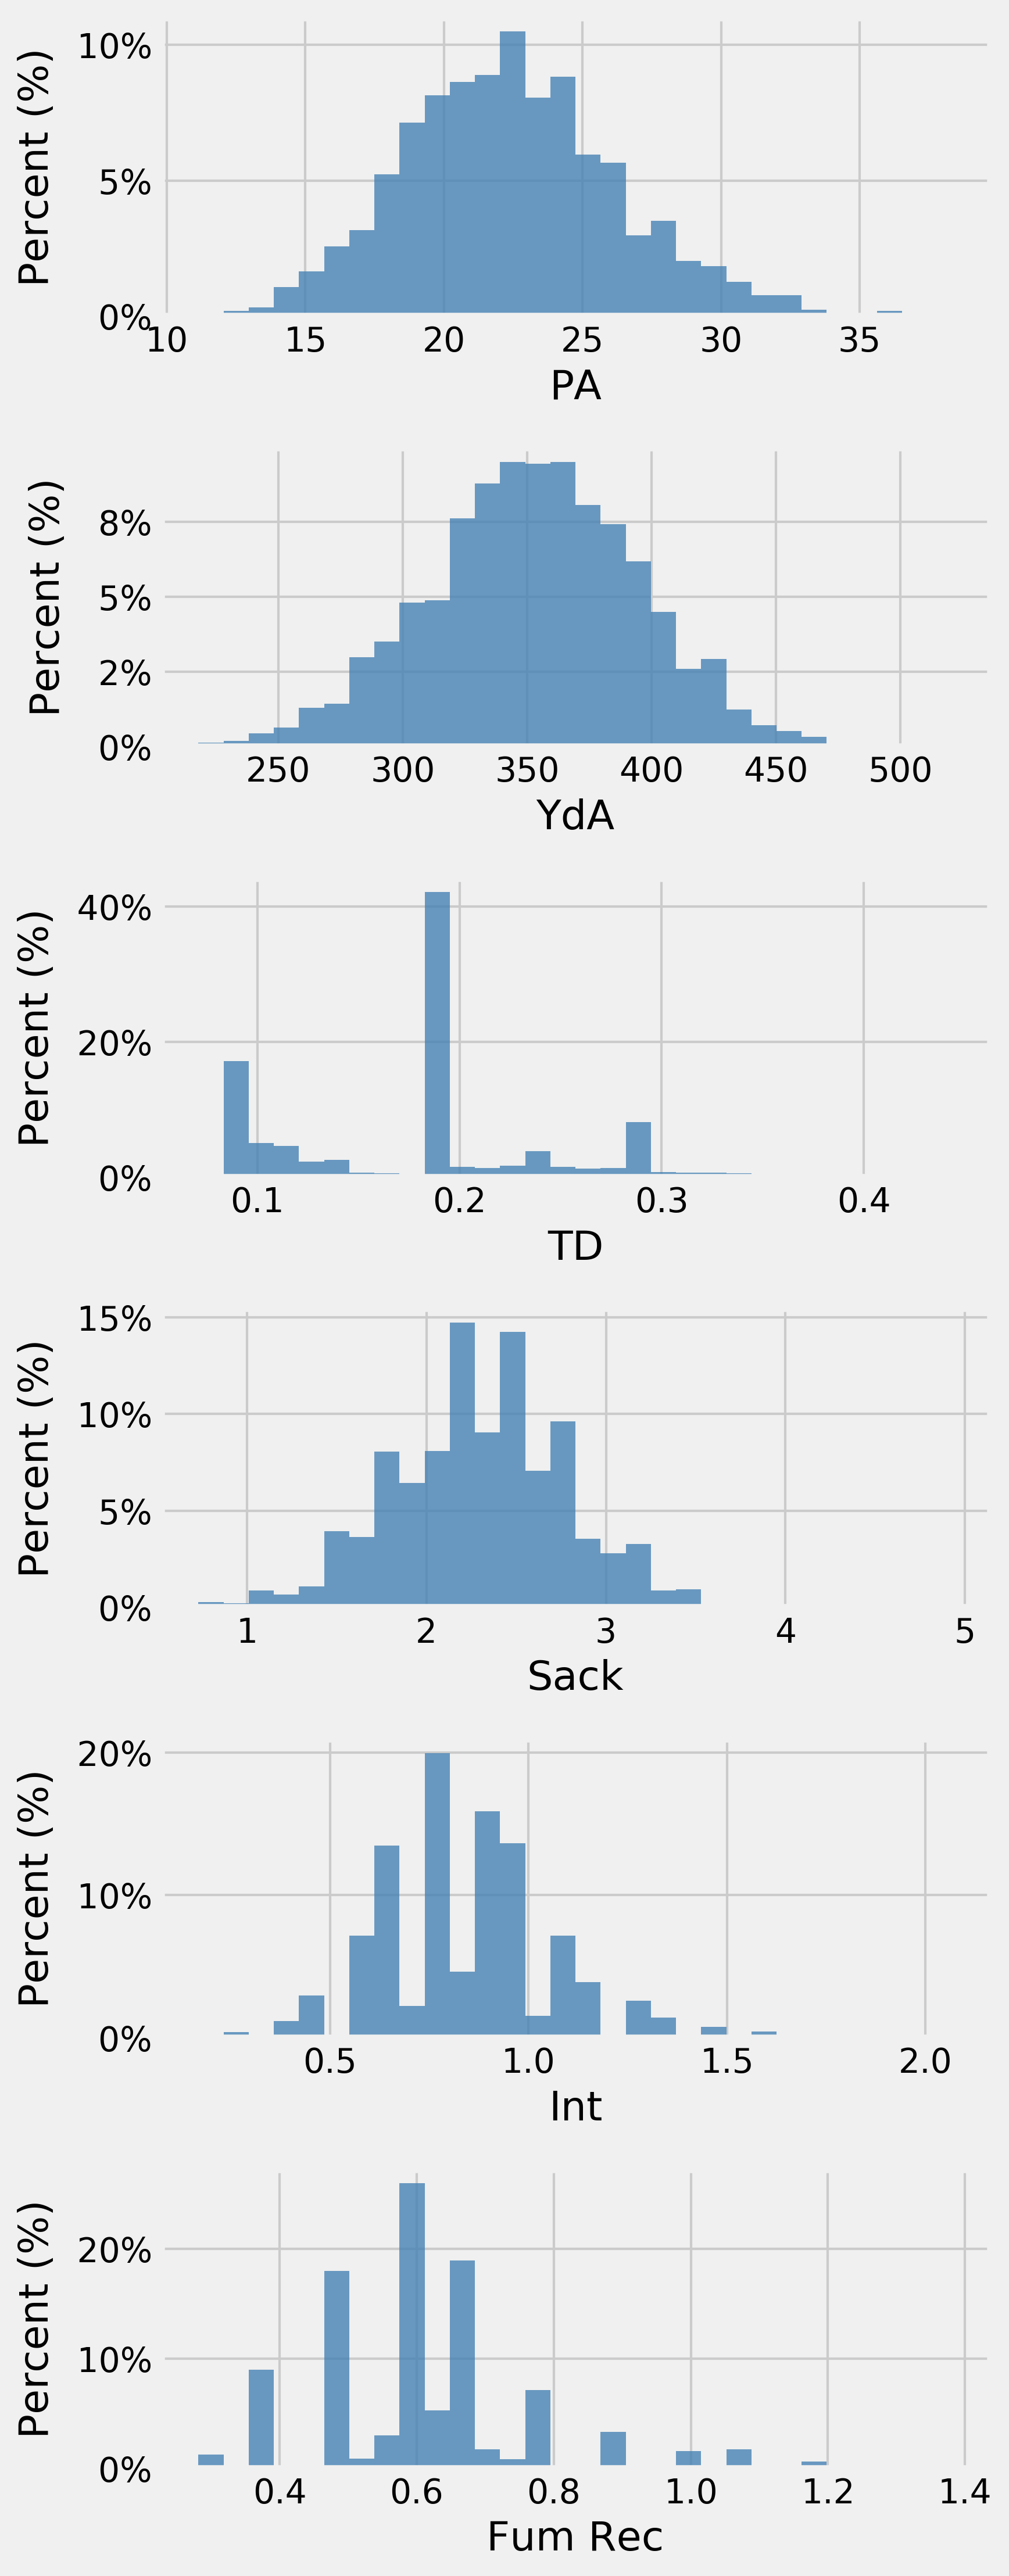
\includegraphics[width=1\textwidth]{../figures/threshold_hist_DST}
    \caption{Histogram above threshold.}
  \end{subfigure}
  \caption{Essential stat raw histograms and thresholded histograms for DST.}
\end{figure}

\pagebreak
\section{Ensemble Results}


\begin{table}[H]
\caption{Ordinary least squares (OLS) regression results for ensemble weighting of each source. Asterisks denote statistical significance of regression coefficients, (*) denoting a p-value less than 0.05, (**) for less than 0.01, and (***) for less than 0.001.}
\centering
\begin{adjustbox}{width =\textwidth}
\begin{tabular}{llllllllll}
\toprule
{} & Position &        Stat &    const &      CBS &     ESPN &  FFToday & FantasyPros &      NFL &    Yahoo \\
\midrule
{} &       QB &    Pass Yds &   -40.48 &    -0.13 &     0.32 &   0.81** &       -0.45 &     0.28 &     0.34 \\
{} &          &     Pass TD &    -0.15 &     0.46 &     0.16 &     0.06 &        0.64 &    -0.28 &     0.08 \\
{} &          &    Pass Int &    -0.01 &     0.11 &    -0.24 &    -0.25 &        0.42 &     0.57 &     0.34 \\
{} &          &    Rush Yds &  3.67*** &     0.15 &    -0.02 &   0.71** &       -0.47 &     0.32 &      0.1 \\
{} &          &     Rush TD &     0.01 &    -0.49 &     0.58 &    -0.17 &        0.33 &     0.87 &    -0.19 \\
{} &       RB &    Rush Yds &     4.38 &     0.02 &   0.44** &    -0.16 &        0.11 &     0.26 &     0.23 \\
{} &          &     Rush TD &     0.06 &     0.27 &    -0.01 &    -0.13 &        0.48 &     0.25 &     0.16 \\
{} &          &  Receptions &     0.08 &     0.12 &   0.3*** &  0.26*** &       -0.05 &     0.18 &  0.17*** \\
{} &          &     Rec Yds &     2.51 &     0.24 &  0.63*** &   0.4*** &       -0.59 &     0.17 &     0.09 \\
{} &          &      Rec TD &     0.03 &    -0.38 &    -0.37 &  -0.36** &        0.98 &  0.76*** &     0.38 \\
{} &       WR &    Rush Yds &   23.23* &     0.18 &   1.47** &        - &        -2.4 &     0.21 &    -0.85 \\
{} &          &  Receptions &     0.23 &  0.29*** &    0.45* &     0.05 &        -0.2 &  0.28*** &     0.07 \\
{} &          &     Rec Yds &     0.82 &    -0.03 &   0.48** &     0.11 &        0.04 &     0.18 &     0.21 \\
{} &          &      Rec TD &     0.03 &     0.03 &  0.51*** &     -0.1 &         0.5 &    -0.04 &     0.09 \\
{} &       TE &  Receptions &  0.36*** &    -0.22 &    -0.07 &     0.07 &        0.45 &    0.56* &     0.08 \\
{} &          &     Rec Yds &     2.62 &    -0.32 &    -0.06 &    -0.29 &     0.96*** &    0.61* &     0.05 \\
{} &          &      Rec TD &  0.08*** &     -0.3 &  0.77*** &     0.08 &       -0.39 &   0.94** &    -0.35 \\
{} &      DST &          PA &     0.05 &     0.31 &        - &        - &         0.1 &    -0.32 &   0.89** \\
{} &          &         YdA &    32.28 &    -0.06 &        - &        - &        0.56 &        - &   0.4*** \\
{} &          &          TD &    -0.19 &     0.15 &    -0.57 &        - &       -0.13 &   3.09** &     0.38 \\
{} &          &        Sack &    -0.43 &     0.07 &     0.08 &        - &       -0.08 &     0.85 &     0.37 \\
{} &          &         Int &     -0.3 &      0.1 &    -0.42 &        - &        1.25 &     0.35 &    -0.06 \\
{} &          &     Fum Rec &     0.52 &     -0.3 &     0.62 &        - &        0.04 &     0.26 &    -0.46 \\
\bottomrule
\end{tabular}
\end{adjustbox}
\end{table}






\end{document}
